\RequirePackage[l2tabu,orthodox]{nag} % This package helps prevent you from doing things wrong.

\documentclass[12pt,a4paper]{article}

\usepackage{ifluatex}
\ifluatex
  \usepackage{fontspec}
  %\setmainfont[Ligatures=TeX]{xits}
  %\setmainfont[Ligatures=TeX]{Latin Modern Roman}
  %\fontspec[SmallCapsFeatures={Letters=SmallCaps}]{Latin Modern Roman}
  \setmainfont[
    BoldFont={TeX Gyre Termes Bold},
    ItalicFont={TeX Gyre Termes Italic},
    BoldItalicFont={TeX Gyre Termes Bold Italic},
    Ligatures=TeX,
    SmallCapsFeatures={Letters=SmallCaps}
    ]{TeX Gyre Termes}

% \setmainfont[
%  Ligatures=TeX
%  BoldFont={Minion Pro Bold},
%  ItalicFont={Minion Pro Italic},
%  BoldItalicFont={Minion Pro Bold Italic}
%  ]{Linux Libertine O}

\else
  \usepackage[utf8]{inputenc}
  %\usepackage[T1]{fontenc}
  %\usepackage{times}
\fi

%\usepackage{fontspec}
\usepackage{amsmath, amssymb, mathtools, contmech}
\usepackage{graphicx, subfig, float, grffile}
\usepackage{algorithm, algorithmic}
\usepackage{microtype}
%\usepackage{todonotes}
\usepackage[width=0.8\paperwidth,height=0.85\paperheight]{geometry}
%\usepackage[firstinits=true, style=alphabetic, url=false, isbn=false, hyperref=true]{biblatex}
%\def\bibfont{\footnotesize}
%\usepackage{siunitx}
%\usepackage{fixltx2e}
%\usepackage{hyperref}
\usepackage{todonotes}
\usepackage{cleveref}
%\usepackage{showkeys} % Shows equation labels!

\usepackage{tikz, pgfplots}
\usetikzlibrary{arrows}

% \renewcommand{\vec}[1]{\mathds{#1}}
% \renewcommand{\mat}[1]{\mathds{#1}}


\ifluatex
  \usepackage{unicode-math}
  %\setmathfont[math-style=ISO]{xits-math.otf}
  %\setmathfont[math-style=ISO]{Asana-Math.otf}
  \setmathfont[math-style=ISO]{latinmodernmath-regular.otf}
  %\setmathfont[math-style=ISO]{texgyretermes-regular.otf}
  \renewcommand{\ta}[1]{\mathbfit{#1}}
  \renewcommand{\ts}[1]{\mathbfit{#1}}
  \renewcommand{\td}[1]{\mathbfcal{#1}}
  \renewcommand{\tf}[1]{\mathbfsfup{#1}}
  \renewcommand{\diff}{\mathbfup{\nabla}}
  \renewcommand{\Box}{\mdlgwhtsquare}
  \renewcommand{\leadsto}{\rightsquigarrow}
\fi

%\captionsetup[subfigure]{textfont=it}
\captionsetup[figure]{textfont=it}
%\newcommand{\figref}[1]{Figure~\ref{#1}}

\linespread{1.3}
\renewcommand{\topfraction}{1.0}	% 99% of page top can be a float
\renewcommand{\bottomfraction}{1.0}	% 99% of page bottom can be a float
\renewcommand{\textfraction}{0.0}	% only 1% of page must to be the text
\renewcommand{\floatpagefraction}{1.0} % 99% of whole page can be a float
\setcounter{totalnumber}{100} %maximum floating objects on one page

% More specialized commands;
\DeclarePairedDelimiter{\homgen}{\langle}{\rangle_\rve}
\DeclarePairedDelimiter{\jmp}{[\![}{]\!]}
\newcommand{\prescribed}{\mathrm{pre}}
\newcommand{\on}{\quad\text{ on }}
\renewcommand{\dev}{\mathrm{d}}
\renewcommand{\vol}{\mathrm{v}}
\newcommand{\per}{\mathrm{per}}
\newcommand{\volume}{|\Omega_\rve|}
\newcommand{\ded}{\mathrm{d}}
\newcommand{\dep}{\mathrm{p}}

% Reduce the size of the rve box a bit:
\newcommand{\rve}{
  {\mathchoice
   {\mbox{\scalebox{0.67}{$\Box$}}}
   {\mbox{\scalebox{0.67}{$\Box$}}}
   {\mbox{\scalebox{0.5}{$\Box$}}}
   {\mbox{\scalebox{0.375}{$\Box$}}}
  }
}
\title{On the Variationally Consistent Computational Homogenization of Elasticity in the Incompressible Limit}

\author{
Mikael Öhman, Fredrik Larsson and Kenneth Runesson\\
Department of Applied Mechanics \\
Chalmers University of Technology}

\begin{document}
\maketitle
\begin{abstract}
The framework for Variationally Consistent Computational (VCH) homogenization of (near-)incompressible solids is discussed.
To focus on the important issues, a model problem of nonlinear (hyper)elasticity and linear kinematics is considered.
A canonical formulation of the RVE-problem is established, whereby complete macroscale incompressibility is obtained straightforwardly as the limit situation.
The framework is sufficiently general to allow for the classical boundary conditions on the RVE as well as the generalized situation of weakly periodic boundary conditions.
Numerical results demonstrating the seamless character of the computational algorithm at the fully incompressible limit conclude the paper.
\end{abstract}

\section{Introduction}

Computational homogenization is a well-established approach in material modeling with the purpose to account for strong micro-heterogeneity in an approximate, yet accurate, fashion without excessive computational cost.
Such an approach can be applied to the situation when the intrinsic material properties are linear, leading to direct ``upscaling''.
It can also be applied to the more complex situation when the subscale properties are nonlinear and/or the subscale problem is inherently transient, whereby it is necessary to resort to nested macro-subscale computation (FE\textsuperscript{2}).
Since the literature on classical as well as computational homogenization is abundant, it is not possible to give a comprehensive account.
Among the seminal work on computational homogenization, we mention \textsc{Miehe (2000)} \cite{Miehe2000}, \textsc{Miehe (2000)} \cite{Miehe2000}, \textsc{Zohdi \& Wriggers (2002)}, ......
Despite the extensive developments, there are still unresolved fundamental issues regarding, for example, (i) variational consistency and the macrohomogeneity condition, (ii) selective homogenization (in particular, for multi-field problems), (iii) how to establish bounds on the effective properties within a given confidence interval, and (iv) rigid inclusions (or pores) in a deformable matrix, for which the classical Dirichlet and Neumann conditions may break down, c.f.\  \textsc{Larsson (2013)} \cite{Lar2013} USNCCM.

The particular aspect considered in this paper, which represents an unresolved issue even in the simplest case of elastic response, is that of Variationally Consistent Homogenization (VCH) in the limit of incompressible micro-constituents.
This situation is encountered when the micro-constituents of a composite are intrinsically incompressible (or nearly incompressible), which infers macroscale incompressibility as well.
An example is when a composite of metallic particles (or fibers) embedded in an elastomer matrix is subjected to stresses that are sufficiently large to cause significant plastic deformations in the particles.
Another class of problems is characterized by an initially compressible macroscale response, which may become incompressible as the result of the deformation process.
An important example is the evolving porous microstructure of a PM-product during the process of sintering, whereby the effective response is compressible until the porosity vanishes inferring incompressible macroscale response.
This process is thus characterized by a transition from the compressible to incompressible regimes that should be handled within the same variational framework, c.f.\  \textsc{Öhman et al.\ (2013)}.

The paper is outlined as follows: The appropriate variational setting of the fine-scale elasticity problem in a mixed format is given in Section 2.
The corresponding VCH framework is outlined in Section 3. .....


\section{Subscale modeling of isotropic elasticity allowing for the incompressible limit}

\subsection{A mixed $(\ta{u},p)$ weak format}

We consider a generic micro-heterogeneous, i.e.\ polycrystalline, material in a given body whose macroscopic configuration occupies the region $\Omega$ in space with (presumed smooth) boundary $\Gamma$.
We are then lead to defining a Statistical Volume Element (SVE), that represents the topology of the micro-heterogeneous microstructure, as shown in \cref{Figure1}.
The total domain occupied by the cubic SVE is denoted $\Omega_\rve$ with external boundary $\Gamma_\rve$.

%-----------------------------------------------------------------------------------------------------------------------------
\begin{figure}
\centering
%\hspace{0.9cm}
%\scalebox{1.0}{
\begin{tikzpicture}
%\tikzstyle{every node}=[font=\Large]
\node [inner sep=0pt,above right]{
   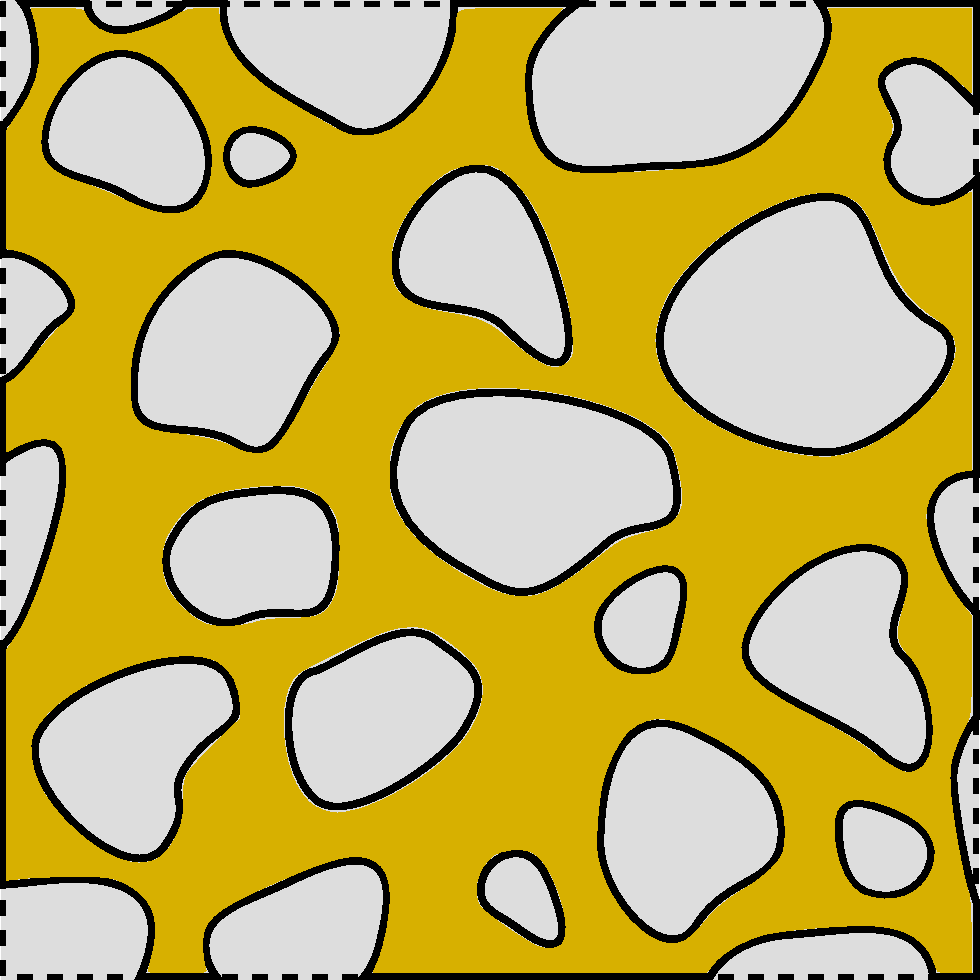
\includegraphics[scale=.3]{SwissCheeseFig}
   };
%\draw[<-, line width=.4mm] (1.6,5.0) .. controls +(up:0.5cm) and +(left:0.5cm) .. (2.5,5.7) node[right=1pt,black,text width=3cm,text badly ragged]{$\Gamma_\rve$};
\draw[<-, line width=.4mm] (5.0,3.5) .. controls +(right:0.5cm) and +(left:0.5cm) .. (6.0,3.0) node[right=1pt,black,text width=3cm,text badly ragged]{$\Gamma_\rve$};
%\draw[-*, line width=.4mm] (-1.0,1.5) node[left=-2.0cm,black,text width=3cm,text badly ragged]{$\Omega_{\rve,i}^\mathrm{p}$} .. controls +(right:0.5cm) and +(left:1.cm) .. (0.6,1.1);
\draw[-*, line width=.4mm] (-1.0,3.0) node[left=-2.1cm,black,text width=3cm,text badly ragged]{$\Omega_\rve$} .. controls +(right:0.5cm) and +(left:1.cm) .. (0.6,2.1);
%\draw[<-, line width=.4mm] (4.6,1.7) .. controls +(right:0.5cm) and +(left:0.5cm) .. (6.0,1.0) node[right=1pt,black,text width=3cm,text badly ragged]{$\partial\Omega_{\rve,i}^\text{p}$};
\end{tikzpicture}
%}
\caption{Generic micro-heterogeneous material consisting of inclusions in matrix (example)}
\label{Figure1}
\end{figure}

We consider a model material as follows: The stress is decomposed in terms of deviator and pressure as $\ts{\sigma} = \ts{\sigma}_\dev - p\ts{I}$.
With the kinematic definition $\ts{\epsilon}_\dev[\ta{u}]\defeq[\ta{u}\outerp\diff]^\sym-\frac{1}{3}[\ta{u}\cdot\diff]\ts{I}$, we introduce the constitutive relations
%------------------------------------------------------------------------------------------------------------
\begin{equation}
    \ts{\sigma}_\dev = \hat{\ts{\sigma}}_\dev(\ts{\epsilon}_\dev[\ta{u}]), \quad
    \ta{u}\cdot\diff = \hat{e}(p)
\label{eq201}
\end{equation}
%------------------------------------------------------------------------------------------------------
Hence, $\hat{\ts{\sigma}}_\dev(\bullet)$ and $\hat{e}(\bullet)$ denote suitable constitutive functions.
Obviously, in the simplest case of linear isotropic elasticity, we have $\hat{\ts{\sigma}}_\dev(\ts{\epsilon}_\dev)=2G\ts{\epsilon}_\dev$ and $\hat{e}(p)=\frac{1}{K}p$, where $G(\ta{x}), K(\ta{x})$ for $\ta{x}\in\Omega$ are the standard elastic moduli that fluctuate strongly.
Moreover, intrinsic incompressibility is defined as $\hat{e}(p)=0$ for any value of $p$.
%------------------------------------------------------------------------------------------------------------------------
We are now in the position to formulate the strong format of the fine-scale problem under standard quasistatic conditions and small strain kinematics:
%------------------------------------------------------------------------------------------------------------
\begin{subequations}\label{eq1}
\begin{alignat}{2}
    -\left[\hat{\ts{\sigma}}_\dev(\ts{\epsilon}_\dev[\ta{u}])-p\ts{I}\right]\cdot\diff & = \ta{f} &&\,\,\text{in}\,\, \Omega
 \label{eq1a} \\
    -\ta{u}\cdot\diff +  \hat{e}(p) & = 0 &&\,\,\text{in}\,\, \Omega
\label{eq1b} \\
    \ta{u} & = \ta{u}_\prescribed &&\,\,\text{on}\,\, \Gamma^\Dirichlet
\label{eq1c} \\
    \ta{t}\defeq\left[\hat{\ts{\sigma}}_\dev(\ts{\epsilon}_\dev[\ta u])-p\ts{I}\right]\cdot\ta{n} & = \ta t_\prescribed &&\,\,\text{on}\,\, \Gamma^\Neumann
\label{eq1d}
\end{alignat}
\end{subequations}
%-----------------------------------------------------------------------------------------------------
The corresponding weak format is: Find $\ta{u}\in\set{U}, p\in\set{P}$ s.t.
%----------------------------------------------------------------------------------------------------------------
\begin{subequations}\label{eq2}
\begin{alignat}{3}
    a(\ta{u};\delta\ta{u}) + b(p,\delta\ta{u}) &= l(\delta\ta{u}) &\quad& \forall \delta\ta{u} &&\in \set{U}^{0}
\label{eq2a} \\
    b(\delta p,\ta{u}) + c^*(p;\delta p) &= 0 &\quad& \forall \delta p &&\in \set{P}
\label{eq2b}
\end{alignat}
\end{subequations}
%----------------------------------------------------------------------------------------------------------------------
where
%----------------------------------------------------------------------------------------------------------------
\begin{align}
    a(\ta{v};\ta{w}) &\defeq
    \int_{\Omega}  \ts{\epsilon}_\dev[\ta{w}]\dprod \hat{\ts{\sigma}}_\dev(\ts{\epsilon}_\dev[\ta{v}]) \dif V
\label{eq3a} \\
    b(q,\ta{v}) &\defeq
    - \int_{\Omega}  q\,\ta{v}\cdot\diff \dif V
\label{eq3b} \\
    c^*(q;r) &\defeq
    \int_{\Omega}  r\,\hat{e}(q) \dif V
\label{eq3c} \\
    l(\ta{v}) &\defeq  \int_{\Omega}  \ta{v}\cdot\ta{f} \dif V + \int_{\Gamma_\Neumann} \ta{v}\cdot \ta t_\prescribed \dif S
\label{eq3d}
\end{align}
%----------------------------------------------------------------------------------------------------------------------
The solution space $\set{U}$ and the test space $\set{U}^0$ are defined in standard fashion.
In particular, all $\ta{v}\in\set{U}$ are characterized by $\ta{v}=\ta{u}_\prescribed$ on $\Gamma_\Dirichlet$, whereas all $\ta{v}\in\set{U}^0$ satisfy $\ta{v}=\ta{0}$ on $\Gamma_\Dirichlet$.
The pressure space $\set{P}$ does not satisfy any boundary conditions.

It is illuminating (although not necessary from an operational point of view) to invoke the potential $\Pi(\ta{u},p)$
%----------------------------------------------------------------------------
\begin{align}
    \Pi(\ta{u},p) &\defeq \Lambda(\ta{u},p) - l(\ta{u})
    \quad\mbox{with}\quad
    \Lambda(\ta{u},p) \defeq \int_{\Omega} \left[\psi_u(\ts{\epsilon}_\dev[\ta{u}]) - p\,\ta{u}\cdot\diff + \psi_p^*(p)\right] \dif V
\label{eq121}
\end{align}
%----------------------------------------------------------------------------
%%----------------------------------------------------------------------------
%\begin{align}
%    \Pi(\ta{u},p) &\defeq
%   \int_{\Omega} \left[\psi_u(\ts{\epsilon}_\dev[\ta{u}]) - p\,\ta{u}\cdot\diff + \psi_p^*(p)\right] \dif V
%   - \int_{\Gamma_\Neumann} l(\ta{u}) \dif S
%\label{eq121}
%\end{align}
%%----------------------------------------------------------------------------
%%----------------------------------------------------------------------------
%\begin{align}
%    \Pi_\rve(\hat{\ta{u}},\hat{p}) &\defeq
%    \frac{1}{\volume}\int_{\Omega_\rve} \left[\psi_u(\ts{\epsilon}_\dev[\hat{\ta{u}}]) - p\,\hat{\ta{u}}\cdot\diff + \psi_p^*(\hat{p})\right] \dif V
%\nonumber \\
%    &= \homgen{ \psi_u(\ts{\epsilon}_\dev[\hat{\ta{u}}])} -
%    \homgen{  p\,\hat{\ta{u}}\cdot\diff } + \homgen{ \psi_p^*(\hat{p})}
%\label{eq4b}
%\end{align}
%%----------------------------------------------------------------------------
where $\psi_u(\ts{\epsilon}_\dev)$ and $\psi_p^*(p)$ are constitutive energy densities\footnote{* indicates ``complementary energy''} such that
%----------------------------------------------------------------------------
\begin{align}
    \hat{\ts{\sigma}}_\dev(\ts{\epsilon}_\dev)=\frac{\partial\psi_u(\ts{\epsilon}_\dev)}{\partial\ts{\epsilon}_\dev}, &\quad
    \hat{e}(p)=\frac{\partial\psi_p^*(p)}{\partial p}
\label{eq122}
\end{align}
%----------------------------------------------------------------------------
The stationarity conditions of $\Pi(\ta{u},p)$ are
%----------------------------------------------------------------------------------------------------------------
\begin{subequations}\label{eq123}
\begin{alignat}{3}
    \Pi'_u(\ta{u},p;\delta\ta{u}) &= a(\ta{u};\delta\ta{u}) + b(p,\delta\ta{u}) - l(\delta\ta{u}) =0 &\quad& \forall \delta\ta{u} &&\in \set{U}^{0}
\label{eq123a} \\
    \Pi'_p(\ta{u},p;\delta p) &= b(\delta p,\ta{u}) + c^*(p;\delta p) = 0 &\quad& \forall \delta p &&\in \set{P}
\label{eq123b}
\end{alignat}
\end{subequations}
%----------------------------------------------------------------------------------------------------------------------
which are identical to the weak form in \cref{eq2}.

\section{Variationally Consistent Homogenization (VCH)}

\subsection{VMS-ansatz and scale separation}

The appropriate variational setting of the homogenized problem is obtained upon replacing the integrands in the weak forms in \crefrange{eq3a}{eq3d} by running averages of the type
%----------------------------------------------------------------------------
\begin{equation}
    y(\bar{\ta{x}}) \mapsto
    \homgen{y}(\bar{\ta{x}})\defeq \frac{1}{|{\Omega}_\rve(\bar{\ta{x}})|}\int_{{\Omega}_\rve} y \dif V, \quad
    \bar{\ta{x}}\in\Omega
    \label{eq16ba}
\end{equation}
%----------------------------------------------------------------------------
representing a smoothing approximation on a Statistical Volume Element (SVE).
In practice, the SVE's are finite-sized and occupies the subscale region $\Omega_\rve(\bar{\ta{x}})$ with boundary $\Gamma_\rve$\footnote{Henceforth, the argument $\bar{\ta{x}}$ is suppressed unless there is a risk of confusion}.
The typical dimension of an SVE is $L_\rve=\volume^{1/3}$.
The SVE is centered at the macroscale position $\bar{\ta{x}}\defeq\frac{1}{|\Gamma_\rve|}\int_{\Gamma_\rve} \ta{x}\dif S$ for any given $\bar{\ta{x}}\in\Omega$.

Boundary integrals can be homogenized in similar fashion, by considering Statistical Surface Elements $\gamma_\rve$
\begin{align}
 y(\bar{\ta x}) \to \langle y \rangle_{||} \defeq \frac{1}{|\gamma_\rve(\bar{\ta x})|} \int_{\gamma_\rve} y \dif S, \quad \bar{\ta x} \in \Gamma
\end{align}


The weak forms in \crefrange{eq3a}{eq3d} are thus approximated as
%----------------------------------------------------------------------------------------------------------------
\begin{align}
    a(\ta{v};\ta{w}) &\approx \int_\Omega a_\rve(\ta{v};\ta{w}) \dif V
\label{eq7a} \\
    b(q,\ta{v}) &\approx \int_\Omega b_\rve(q,\ta{v}) \dif V
\label{eq7b} \\
    c^*(q;r) &\approx \int_\Omega c^*_\rve(q;r) \dif V
\label{eq7c} \\
    l(\ta{v}) &\approx \int_\Omega l_\rve(\ta{v}) \dif V + \int_{\Gamma_\Neumann} l_\parallel(\ta{v}) \dif S
\label{eq7d}
\end{align}
%---------------------------------------------------------------------------------------------------------------------
where the SVE-functionals in \crefrange{eq7a}{eq7d} are defined as
%----------------------------------------------------------------------------------------------------------------
\begin{align}
    a_\rve(\ta{v};\ta{w}) &\defeq
    \homgen{ \ts{\epsilon}_\dev[\ta{w}]\dprod \hat{\ts{\sigma}}_\dev(\ts{\epsilon}_\dev[\ta{v}]) }
\label{eq8a} \\
    b_\rve(q,\ta{v}) &\defeq
    -  \homgen{ q\,\ta{v}\cdot\diff }
\label{eq8b} \\
    c^*_\rve(q;r) &\defeq
    \homgen{ r\,\hat{e}(q) }
\label{eq8c} \\
    l_\rve(\ta{v}) &\defeq
    \homgen{ \ta{v}\cdot\ta{f} }, \quad
    l_\parallel(\ta{v}) \defeq
    \langle \ta{v}\cdot \ta t_\prescribed \rangle_{||}
\label{eq8d}
\end{align}
%---------------------------------------------------------------------------------------------------------------------
Likewise, we homogenize the volumetric energy potential $\Lambda(\ta{u},p)$:
%----------------------------------------------------------------------------
\begin{align}
    \Lambda(\ta{v},q) &\approx \int_\Omega \Lambda_\rve(\ta{v},q) \dif V
\label{eq222}
\end{align}
%----------------------------------------------------------------------------
where the SVE-functional $\Lambda_\rve(\ta{v},q)$ is given as
%----------------------------------------------------------------------------
\begin{align}
    \Lambda_\rve(\ta{v},q) &\defeq
    \homgen{ \psi_u(\ts{\epsilon}_\dev[\ta{v}])} -
    \homgen{  p\,\ta{v}\cdot\diff } + \homgen{ \psi_p^*(q) }
\label{eqRveBulkPotential}
\end{align}
%----------------------------------------------------------------------------

In the spirit of the Variational MultiScale method (VMS), we introduce the \emph{ansatz} that the fields $\ta{u}\in\set{U}$ and $p\in\set{P}$ can be decomposed into macroscale (smooth) and subscale (fluctuating) parts inside each SVE via the unique orthogonal split $\set{U} = \set{U}^\macro \oplus \set{U}^\fluct$ and $\set{P} = \set{P}^\macro \oplus \set{P}^\fluct$.
In practice, the scales are linked  by expressing $\ta{u}^\macro(\bar{\ta{x}},{\ta{x}})$\footnote{Double arguments, i.e.\ $\ta{u}(\bar{\ta{x}},\ta{x})$, are used to explicitly point out the underlying scale separation.} using Taylor series expansions of suitable order for $\bar{\ta{x}}\in\Omega$ and $\ta{x}\in\Omega_\rve(\bar{\ta{x}})$
in terms of the macroscale solution $\bar{\ta{u}}(\bar{\ta{x}})$ in an explicit fashion and defining the \emph{approximate} solution $\ta{u}^\fluct=\ta{u}^\fluct\{\bar{\ta{u}}\}$\footnote{Curly brackets $\{(\bullet)\}$ indicate implicit and/or nonlocal functional dependence on $(\bullet)$.} for given $\bar{\ta{u}}$.
This (implicit) relation allows for computing the homogenized quantities.

As a result, we may assume that it is possible solve for the fluctuation fields $\ta{u}^\fluct\in\set{U}^\fluct$ and $p^\fluct\in\set{P}^\fluct$ as ``local approximations'' on each SVE for given macroscale solutions $\ta{u}^\macro\in\set{U}^\macro$ and $p^\macro\in\set{P}^\macro$, i.e.\ we construct the complete solution on each SVE as\footnote{Curly brackets indicate implicit function}.
%------------------------------------------------------------------------------------------------------------
\begin{subequations}\label{eq4}
\begin{alignat}{2}
    \ta{u}\approx \tilde{\ta{u}}\{\ta{u}^\macro,p^\macro\} &\defeq \ta{u}^\macro+\tilde{\ta{u}}^\fluct\{\ta{u}^\macro,p^\macro\} &&\text{ in } \Omega_\rve
\label{eq4a} \\
    p\approx \tilde{p}\{\ta{u}^\macro,p^\macro\} &\defeq p^\macro+\tilde{p}^\fluct\{\ta{u}^\macro,p^\macro\} &&\text{ in } \Omega_\rve
\label{eq4b}
\end{alignat}
\end{subequations}
%------------------------------------------------------------------------------------------------------------
On the boundary of the macroscale domain, $\Gamma$, we assume smooth variation of $\ta{u}$ defined as by the explicit relations $\ta u = \ta u^\macro$, $p = p^\macro$ on $\gamma_\rve$.


In addition, the test function $\delta\ta{u}\in\set{U}^{0}$ in \cref{eq2a} is replaced by $\delta\ta{u}^\macro\in\set{U}^{\macro,0}$, whereas $\delta p\in\set{P}$ in \cref{eq2b} is replaced by $\delta p^\macro\in\set{P}^{\macro}$.
Altogether, these assumptions infer that $\ta{u}^\macro\in\set{U}^\macro$ and $p^\macro\in\set{P}^\macro$ can be solved from the homogenized problem
%----------------------------------------------------------------------------------------------------------------
\begin{subequations}\label{eq6}
\begin{alignat}{3}
    a(\tilde{\ta{u}}\{\ta{u}^\macro,p^\macro\};\delta\ta{u}^\macro) +
    b(\tilde{p}\{\ta{u}^\macro,p^\macro\},\delta\ta{u}^\macro)
    &= l(\delta\ta{u}^\macro)
    &\quad& \forall \delta\ta{u}^\macro &&\in \set{U}^{\macro,0}
\label{eq6a} \\
    b(\delta p^\macro,\tilde{\ta{u}}\{\ta{u}^\macro,p^\macro\}) +
    c^*(\tilde{p}\{\ta{u}^\macro,p^\macro\};\delta p^\macro)
    &= 0 &\quad& \forall \delta p^\macro &&\in \set{P}^{\macro}
\label{eq6b}
\end{alignat}
\end{subequations}
%----------------------------------------------------------------------------------------------------------------------
%----------------------------------------------------------------------------------------------------------------
%\begin{subequations}\label{eq6}
%\begin{alignat}{3}
%    a(\ta{u}^\macro+\tilde{\ta{u}}^\fluct\{\ta{u}^\macro,p^\macro\};\delta\ta{u}^\macro) +
%    b(\delta\ta{u}^\macro,p^\macro+\tilde{p}^\fluct\{\ta{u}^\macro,p^\macro\})
%    &= l(\delta\ta{u}^\macro)
%    &\quad& \forall \delta\ta{u}^\macro &&\in \set{U}^{\macro,0}
%\label{eq6a} \\
%    b(\ta{u}^\macro+\tilde{\ta{u}}^\fluct\{\ta{u}^\macro,p^\macro\};\delta p^\macro) +
%    c^*(p^\macro+\tilde{p}^\fluct\{\ta{u}^\macro,p^\macro\};\delta p^\macro)
%    &= 0 &\quad& \forall \delta p^\macro &&\in \set{P}^{\macro}
%\label{eq6b}
%\end{alignat}
%\end{subequations}
%----------------------------------------------------------------------------------------------------------------------
%\textbf{Remark}: For technical simplicity, it is assumed that the boundary data are smooth such that $l_\parallel(\ta{v})=l_\parallel(\ta{v}^\macro)$. $\Box$

%\subsection{Variationally Consistent Macrohomogeneity Condition (VCMC)}
%\todo{UP-DATE}
%
%The classical Hill-Mandel, or macrohomogeneity, condition for elasticity ensures the equivalence of elastic energy of the fine-scale and the homogenized formulations.
%This advantageous homogenization property can be generalized within the framework of VMM.
%We thus introduce the notion of Variationally Consistent Macrohomogeneity Condition (VCMC), which must be satisfied for the RVE-problems.
%As a consequence, symmetry is preserved of the macroscale tangent stiffness in the case that the fine-scale problem is associated with a (local) potential.
%This holds true in the present case of (nonlinear) elasticity; however, it applies also to a number of more complex problem formulations including those of standard dissipative material.
%Such symmetry carries over to a Galerkin property for the FE-discretized macroscale problem.
%
%In order to formulate the VCMC, we introduce the \emph{sensitivities} of the fluctuation fields.
%For example, $(\tilde{\ta{u}}^\fluct)_u'\{\ta{u}^\macro,p^\macro;\dif\ta{u}^\macro\}$ is the directional derivative of $\tilde{\ta{u}}^\fluct$ for a differential change $\dif\ta{u}^\macro$.
%Upon introducing the approximations for $\ta{u}$ and $p$ as given in \eqref{eq4}, we conclude that the stationary conditions of $\Pi(\tilde{\ta{u}}\{\ta{u}^\macro,p^\macro\},\tilde{p}\{\ta{u}^\macro,p^\macro\})$ are given as
%%%----------------------------------------------------------------------------------------------------------------
%%\begin{subequations}\label{eq9}
%%\begin{alignat}{3}
%%    (\dif\tilde{\ta{u}}^\fluct)_u &\defeq (\tilde{\ta{u}}^\fluct)_u'\{\ta{u}^\macro,p^\macro;\dif\ta{u}^\macro\},
%%    (\dif\tilde{p}^\fluct)_u &\defeq (\tilde{p}^\fluct)_u'\{\ta{u}^\macro,p^\macro;\dif\ta{u}^\macro\},  \,\,
%%    &\dif\ta{u}^\macro\in \set{U}^{\macro,0}
%%\label{eq9a} \\
%%    (\dif\tilde{\ta{u}}^\fluct)_p &\defeq (\tilde{\ta{u}}^\fluct)_p'\{\ta{u}^\macro,p^\macro;\dif p^\macro\},
%%    (\dif\tilde{p}^\fluct)_p &\defeq (\tilde{p}^\fluct)_p'\{\ta{u}^\macro,p^\macro;\dif p^\macro\}, \,\,
%%    &\dif p^\macro\in \set{P}^{\macro}
%%\label{eq9b}
%%\end{alignat}
%%\end{subequations}
%%%----------------------------------------------------------------------------------------------------------------------
%%----------------------------------------------------------------------------------------------------------------
%\begin{subequations}\label{eq110}
%\begin{alignat}{3}
%    \Pi'_u(\bullet;\delta\ta{u}^\macro) + \Pi'_u(\bullet;(\tilde{\ta{u}}^\fluct)_u'\{\ta{u}^\macro,p^\macro;\delta\ta{u}^\macro\} + (\tilde{p}^\fluct)_u'\{\ta{u}^\macro,p^\macro;\delta\ta{u}^\macro\})
%    = 0
%    &\quad& \forall \delta\ta{u}^\macro &&\in \set{U}^{\macro,0}
%\label{eq110a} \\
%    \Pi'_p(\bullet;\delta p^\macro) + \Pi'_p(\bullet;(\tilde{\ta{u}}^\fluct)_p'\{\ta{u}^\macro,p^\macro;\delta p^\macro\} + (\tilde{p}^\fluct)_p'\{\ta{u}^\macro,p^\macro;\delta p^\macro\})
%    = 0
%    &\quad& \forall \delta p^\macro &&\in \set{P}^{\macro}
%\label{eq110b}
%\end{alignat}
%\end{subequations}
%%----------------------------------------------------------------------------------------------------------------------
%With the identities $R^{(u)}=\Pi'_u$, $R^{(p)}=\Pi'_p$ it is clear that the homogenization problem already established in \eqref{eq6} can be written
%%----------------------------------------------------------------------------------------------------------------
%\begin{subequations}\label{eq111}
%\begin{alignat}{3}
%    R^{(u)}(\bullet;\delta\ta{u}^\macro)
%    = 0
%    &\quad& \forall \delta\ta{u}^\macro &&\in \set{U}^{\macro,0}
%\label{eq111a} \\
%    R^{(p)}(\bullet;\delta p^\macro)
%    = 0
%    &\quad& \forall \delta p^\macro &&\in \set{P}^{\macro}
%\label{eq111b}
%\end{alignat}
%\end{subequations}
%%----------------------------------------------------------------------------------------------------------------------
%Moreover, the localized form of the VCMC is
%%----------------------------------------------------------------------------------------------------------------
%\begin{subequations}\label{eq112}
%\begin{alignat}{3}
%    R_\rve^{(u)}(\bullet;(\tilde{\ta{u}}^\fluct)_u'\{\ta{u}^\macro,p^\macro;\delta\ta{u}^\macro\} + (\tilde{p}^\fluct)_u'\{\ta{u}^\macro,p^\macro;\delta\ta{u}^\macro\})
%    = 0
%    &\quad& \forall \delta\ta{u}^\macro &&\in \set{U}^{\macro,0}|_{\Omega_\rve}
%\label{eq112a} \\
%    R_\rve^{(p)}(\bullet;(\tilde{\ta{u}}^\fluct)_p'\{\ta{u}^\macro,p^\macro;\delta p^\macro\} +
%    (\tilde{p}^\fluct)_p'\{\ta{u}^\macro,p^\macro;\delta p^\macro\})
%    = 0
%    &\quad& \forall \delta p^\macro &&\in \set{P}^{\macro}|_{\Omega_\rve}
%\label{eq112b}
%\end{alignat}
%\end{subequations}
%%----------------------------------------------------------------------------------------------------------------------
%which can be expressed explicitly as
%%\footnote{No distinction is made henceforth between $\ta{u}$ and $\tilde{\ta{u}}$, etc.}
%%----------------------------------------------------------------------------------------------------------------
%\begin{subequations}\label{eq115}
%\begin{align}
%    &a_\rve(\tilde{\ta{u}}\{\ta{u}^\macro,p^\macro\};(\tilde{\ta{u}}^\fluct)_u'\{\ta{u}^\macro,p^\macro;\delta\ta{u}^\macro\})
%\nonumber\\
%    &+ b_\rve(\tilde{p}\{\ta{u}^\macro,p^\macro\},(\tilde{\ta{u}}^\fluct)_u'\{\ta{u}^\macro,p^\macro;\delta\ta{u}^\macro\}) +  b_\rve((\tilde{p}^\fluct)_u'\{\ta{u}^\macro,p^\macro;\delta\ta{u}^\macro\},\tilde{\ta{u}}\{\ta{u}^\macro,p^\macro\})
%\nonumber \\
%    &+ c^*_\rve(\tilde{p}\{\ta{u}^\macro,p^\macro\};(\tilde{p}^\fluct)_u'\{\ta{u}^\macro,p^\macro;\delta\ta{u}^\macro\})
%    = l_\rve((\tilde{\ta{u}}^\fluct)_u'\{\ta{u}^\macro,p^\macro;\delta\ta{u}^\macro\})
%\nonumber \\
%    &\quad \forall \ta{u}^\macro,p^\macro,\delta\ta{u}^\macro \in \set{U}^{\macro}|_{\Omega_\rve}\times\set{P}^{\macro}|_{\Omega_\rve}\times\set{U}^{\macro,0}|_{\Omega_\rve}
%\label{eq115a} \\
%    &a_\rve(\tilde{\ta{u}}\{\ta{u}^\macro,p^\macro\};(\tilde{\ta{u}}^\fluct)_p'\{\ta{u}^\macro,p^\macro;\delta p^\macro\})
%\nonumber \\
%    &+ b_\rve(\tilde{p}\{\ta{u}^\macro,p^\macro\},(\tilde{\ta{u}}^\fluct)_p'\{\ta{u}^\macro,p^\macro;\delta p^\macro\}) +
%    b_\rve((\tilde{p}^\fluct)_p'\{\ta{u}^\macro,p^\macro;\delta p^\macro\},\tilde{\ta{u}}\{\ta{u}^\macro,p^\macro\})
%\nonumber \\
%    &+ c^*_\rve(\tilde{p}\{\ta{u}^\macro,p^\macro\};(\tilde{p}^\fluct)_p'\{\ta{u}^\macro,p^\macro;\delta p^\macro\})
%    = l_\rve((\tilde{\ta{u}}^\fluct)_p'\{\ta{u}^\macro,p^\macro;\delta p^\macro\})
%\nonumber \\
%    &\quad \forall \ta{u}^\macro,p^\macro,\delta p^\macro \in
%    \set{U}^{\macro}|_{\Omega_\rve}\times\set{P}^{\macro}|_{\Omega_\rve}\times\set{P}^{\macro}|_{\Omega_\rve}
%\label{eq115b}
%\end{align}
%\end{subequations}
%%----------------------------------------------------------------------------------------------------------------------
%
%\textbf{Remark}: The partial sensitivities $(\tilde{\ta{u}}^\fluct)'_u, (\tilde{p}^\fluct)'_u$ for a given $\dif\ta{u}^\macro\in \set{U}^{\macro,0}$ and $(\tilde{\ta{u}}^\fluct)'_p, (\tilde{p}^\fluct)'_p$ for a given $\dif p^\macro\in \set{P}^{\macro}$ can be solved from ``tangent problems'' that represent the linearization of the appropriately formulated subscale problem to be solved on each SVE.
%It is then clear that \cref{eq115} represent the weakest possible form of the VCMC when this condition is localized to each SVE.
%However, it is common procedure to establish the boundary conditions for the actual RVE-problem in such a fashion that the equations in \cref{eq115} are satisfied for a larger class of test functions than those in the tangent spaces, see below. $\Box$
%%%----------------------------------------------------------------------------------------------------------------
%%\begin{equation}
%%%    a_\rve(\ta{u},\left(\ta{u}^\fluct\right)'\{\ta{u}^\macro;\delta \ta{u}^\macro\}) = 0 \quad \forall \delta \ta{u}^\macro \in \set{U}^{\macro,0}
%%    a(\ta{u},\delta\tilde{\ta{u}}^\fluct) =
%%    \frac{1}{\volume} \int_{\Omega_\rve^\fluct} \delta\tilde{\ts{\epsilon}}^\fluct\dprod\ts{\sigma}(\ts{\epsilon}) \dif V
%%    = 0 \quad \forall \delta \ta{u}^\macro \in \set{U}^{\macro,0}
%%\label{eq10}
%%\end{equation}
%%%----------------------------------------------------------------------------------------------------------------------
%%
%%Upon using the divergence theorem in \cref{eq10} and strong equilibrium, we may obtain the useful alternative condition
%%%----------------------------------------------------------------------------------------------------------------
%%\begin{equation}
%%  \frac{1}{\volume} \int_{\Gamma_\rve^\fluct} \ta{t} \cdot \delta\tilde{\ta{u}}^\fluct \dif S = 0
%%  \quad \forall \delta \ta{u}^\macro \in \set{U}^{\macro,0}
%%\label{eq11}
%%\end{equation}
%%%----------------------------------------------------------------------------------------------------------------------
%%which is satisfied for suitable (i) model assumption on the traction $\ta{t}$ and/or (ii) restriction on the the test function $\delta \tilde{\ta{u}}^\fluct \defeq \left(\tilde{\ta{u}}^\fluct\right)'\{\ta{u}^\macro;\delta \ta{u}^\macro\}$.

\subsection{Explicit format of macroscale (homogenized) problem}

We shall consider the homogenization properties on a given SVE and introduce the macroscale fields $(\bar{\ta{u}},\bar{p})\in\bar{\set{U}}\times\bar{\set{P}}$ such that the macroscale solutions $\ta{u}^\macro, p^\macro$ inside each SVE are expanded as follows:
%----------------------------------------------------------------------------
\begin{subequations}\label{eq12}
\begin{align}
    \ta{u}^\macro(\bar{\ta{x}};\ta{x}) &= \bar{\ta{u}}(\bar{\ta{x}}) + \bar{\ts{h}}(\bar{\ta{x}}) \cdot [\ta{x}-\bar{\ta{x}}], \quad \bar{\ts{h}}\defeq\bar{\ta{u}}\outerp\diff, \quad \ta{x}\in\Omega_\rve
\label{eq12a} \\
    p^\macro(\bar{\ta{x}};\ta{x}) &= \bar{p}(\bar{\ta{x}}) \quad
    \ta{x}\in\Omega_\rve
\label{eq12b}
\end{align}
\end{subequations}
%----------------------------------------------------------------------------
Hence, $\ta{u}^\macro$ is assumed to have linear variation in $\Omega_\rve$ pertinent to standard ``first order homogenization'', whereas $p^\macro$ is constant in $\Omega_\rve$.
As to the fluctuation fields, we introduce the constraints
%----------------------------------------------------------------------------
\begin{align}
    \frac{1}{|\Gamma_\rve|} \int_{\Gamma_\rve} \ta{u}^\fluct \dif S &= \ta{0}, \quad
    \frac{1}{\volume} \int_{\Omega_\rve} \ta{u}^\fluct\outerp\diff \dif V = \ta{0}
\label{eq13a} \\
    \frac{1}{\volume} \int_{\Omega_\rve} p^\fluct\dif V &= 0
\label{eq13b}
\end{align}
%----------------------------------------------------------------------------
As a result, the hierarchical split $\set{U} = \set{U}^\macro \oplus \set{U}^\fluct$ and $\set{P} = \set{P}^\macro \oplus \set{P}^\fluct$ is guaranteed.
We thus obtain
%----------------------------------------------------------------------------
\begin{align}
    \bar{\ta{u}} &=\frac{1}{|\Gamma_\rve|} \int_{\Gamma_\rve} \ta{u} \dif S, \quad
    \bar{\ta{h}} =\frac{1}{\volume} \int_{\Omega_\rve} \ta{u}\outerp\diff \dif V
\label{eq14a} \\
    \bar{p} &=\frac{1}{\volume} \int_{\Omega_\rve} p \dif V
\label{eq14b}
\end{align}
%----------------------------------------------------------------------------
We can thus establish at the outset, before any further analysis, that the displacement and pressure fields within each SVE are implicit functions of the values $\bar{\ta u}$, $\bar{\ts h}$, $\bar{p}$, such that
$\ta u = \tilde{\ta u}\{\bar{\ta u}, \bar{\ts h}, \bar{p}\}$ and $p = \tilde{p}\{\bar{\ta u}, \bar{\ts h}, \bar{p}\}$.
%%----------------------------------------------------------------------------
%\begin{subequations}
%\begin{align}
% \ta u = \tilde{\ta u}\{\bar{\ta u}, \bar{\ts h}, \bar{p}\}
%\\
% p = \tilde{p}\{\bar{\ta u}, \bar{\ts h}, \bar{p}\}
%\end{align}
%\end{subequations}
%%----------------------------------------------------------------------------

Finally, we are in the position to compute the homogenized quantities that enter the system \cref{eq6}:
%----------------------------------------------------------------------------------------------------------------
%\todo{$\delta u^\macro$ in RHS but not in LHS}
\begin{align}
    a_\rve(\ta{u};\delta\ta{u}^\macro) &=
%    \homgen{ \ts{\epsilon}_\dev[\delta\bar{\ta{u}}]\dprod \hat{\ts{\sigma}}_\dev(\ts{\epsilon}_\dev[\ta{u}]) } =
    \ts{\epsilon}_\dev[\delta\bar{\ta{u}}] \dprod \bar{\ts{\sigma}}_\dev
\label{eq15a} \\
    b_\rve(p,\delta\ta{u}^\macro) &=
%    -  \homgen{ p\,\delta\bar{\ta{u}}\cdot\diff } =
    - \bar{p}\,\delta\bar{\ta{u}}\cdot\diff
\label{eq15b} \\
    b_\rve(\delta p^\macro,\ta{u}) &=
%    -  \homgen{ \delta\bar{p}\,\ta{u}\cdot\diff } =
    - \delta\bar{p}\,\bar{\ta{u}}\cdot\diff
\label{eq15c} \\
    c^*_\rve(p;\delta p^\macro) &=
%    \homgen{ \delta\bar{p}\,\hat{e}(p) } =
    \delta\bar{p}\,\bar{e}
\label{eq15d} \\
    l_\rve(\delta\ta{u}^\macro) &=
%    \homgen{ \delta\bar{\ta{u}}\cdot\ta{f} } + \homgen{[\delta\bar{\ta{u}}\outerp\diff]\dprod\left[\ta{f}\outerp[\ta{x}-\bar{\ta{x}}]\right] } =
    \delta\bar{\ta{u}}\cdot \bar{\ta f} + [\delta\bar{\ta{u}}\outerp\diff]\dprod \bar{\bar{\ta f}}
\label{eq15e} \\
    l_\parallel(\delta\ta{u}^\macro) &=
    \delta\bar{\ta{u}} \cdot \bar{\ta t}_\prescribed + [\delta\bar{\ta u}\outerp\diff]\dprod \bar{\bar{\ta{t}}}_\prescribed
\label{eq15f}
\end{align}
%---------------------------------------------------------------------------------------------------------------------
The applied macroscale load $\bar{\ta f}$ and ``moment'' $\bar{\bar{\ta f}}$ are defined as
%----------------------------------------------------------------------------------------------------------------
\begin{alignat}{2}
    \bar{\ta f} &= \homgen{ \ta{f} },\quad
    &\bar{\bar{\ta f}} &= \homgen{ \ta{f}\outerp[\ta{x}-\bar{\ta{x}}] }
\label{eq15fa}
\\
    \bar{\ta t} &= \langle \ta{t} \rangle_{||},\quad
    &\bar{\bar{\ta t}} &= \langle \ta{t}\outerp[\ta{x}-\bar{\ta{x}}]  \rangle_{||}
\end{alignat}
%---------------------------------------------------------------------------------------------------------------------
\textbf{Remark:} Henceforth, we restrict to the situation when $|\gamma_\rve|\to 0$; hence $\bar{\bar{\ta f}}$ and $\bar{\bar{\ta t}}$ vanish.
We will also focus on the homogenization of $\bar{\ts\sigma}_\dev$ and $\bar{e}$, so $\bar{\ta t}$ and $\bar{\ta f}$ are considered as given macroscopic quantities.

The variationally consistent macroscale ``flux'' variables $\bar{\ts{\sigma}}_\dev$ and $\bar{e}$ are obtained from homogenization of the constitutive functions as follows:
%----------------------------------------------------------------------------------------------------------------
\begin{subequations}\label{eq16}
\begin{align}
    \bar{\ts{\sigma}}_\dev &\defeq \homgen{ \hat{\ts{\sigma}}_\dev(\ts{\epsilon}_\dev[\ta{u}]) }
\label{eq16a} \\
    \bar{e} &\defeq \homgen{ \hat{e}(p) }
\label{eq16b}
\end{align}
\end{subequations}
%----------------------------------------------------------------------------------------------------------------
By combining \eqref{eq4} with \eqref{eq12} we note that $\bar{\ts\sigma}_\dev$ and $\bar{e}$ are indeed implicit functions of the values of the macroscale variables $\bar{\ta u}$, $\bar{\ts h}$ and $\bar{p}$, pertinent to the considered SVE.

Moreover, in order to obtain \cref{eq15b,eq15c} we used the identities
%----------------------------------------------------------------------------------------------------------------
\begin{equation}
%    \bar{p} = \homgen{ p }, \quad \bar{\ta{u}}\cdot\diff = \homgen{ \ta{u}\cdot\diff }
    \bar{p} = \homgen{ p }, \quad \bar{h}_\vol \defeq \bar{\ta{u}}\cdot\diff = \homgen{ \ta{u}\cdot\diff }
\label{eq16c}
\end{equation}
%---------------------------------------------------------------------------------------------------------------------

Finally, upon inserting \crefrange{eq15a}{eq15f} into the system \cref{eq6}, we obtain the macroscale problem:
Find $(\bar{\ta{u}},\bar{p})\in\bar{\set{U}}\times\bar{\set{P}}$ that solve
%----------------------------------------------------------------------------------------------------------------
\begin{subequations}\label{eq17}
\begin{alignat}{3}
    \bar{a}(\bar{\ta{u}},\bar{p};\delta\bar{\ta{u}}) + \bar{b}(\bar{p},\delta\bar{\ta{u}}) &= \bar{l}(\delta\bar{\ta{u}})
      &\quad& \forall \delta\bar{\ta{u}} &&\in \bar{\set{U}}^{0}
\label{eq17a} \\
    \bar{b}(\delta\bar{p},\bar{\ta{u}}) + \bar{c}^*(\bar{\ta{u}},\bar{p};\delta\bar{p}) &= 0
      &\quad& \forall \delta\bar{p} &&\in \bar{\set{P}}
\label{eq17b}
\end{alignat}
\end{subequations}
%----------------------------------------------------------------------------------------------------------------------
where
%----------------------------------------------------------------------------------------------------------------
\begin{align}
    \bar{a}(\bar{\ta{u}},\bar{p};\bar{\ta w}) &\defeq
    \int_{\Omega}  \ts{\epsilon}_\dev[\bar{\ta w}]\dprod\bar{\ts\sigma}_\dev\{\bar{\ta u}, \bar{p}\} \dif V
\label{eq18a} \\
    \bar{b}(\bar{q},\bar{\ta u}) &\defeq
    - \int_{\Omega}  \bar{q}\,\bar{\ta{u}}\cdot\diff \dif V
\label{eq18b} \\
    \bar{c}^*(\bar{\ta{u}},\bar{p};\bar{r}) &\defeq
    \int_{\Omega}  \bar{r}\,\bar{e}\{\bar{\ta u}, \bar{p}\} \dif V
\label{eq18c} \\
    \bar{l}(\bar{\ta u}) &\defeq  \int_{\Omega}  \bar{\ta u}\cdot\bar{\ta f} \dif V +
    \int_{\Gamma^\Neumann} \bar{\ta u}\cdot\bar{\ta t}_\prescribed \dif S
\label{eq18d}
\end{align}
%----------------------------------------------------------------------------------------------------------------------
If we consider the macroscale fields, $\bar{\ts\sigma}_\dev$ and $\bar{e}$,  we conclude that they are implicit functions of the fields $\bar{\ta u}$ and $\bar{p}$.
The macroscale spaces $\bar{\set{U}}$ and $\bar{\set{P}}$ are chosen as the standard ones for the fine-scale problem.

\section{Canonical formulation of RVE-problem}

\subsection{Preliminaries -- Concept of weak periodicity of fluctuation displacement}

To avoid unnecessary technical complexity, we henceforth consider the situation without volume load, i.e.\ $\ta{f}=\ta{0}$.
As a preliminary for establishing the proper variational format of the RVE-problem, we consider the most general weak form of the quasi-static momentum balance by introducing the boundary integral with boundary tractions:
%----------------------------------------------------------------------------
\begin{subequations}
\begin{align}
    a_\rve(\ta{u};\delta\ta{u}) + b_\rve(\delta\ta{u},p) - \frac{1}{\volume}\int_{\Gamma_\rve} \ta{t}\cdot\delta\ta{u} \dif S &= 0
\label{eq19a} \\
    b_\rve(\ta{u},\delta p) + c^*_\rve(p;\delta p) &= 0
\label{eq19b}
\end{align}
\end{subequations}
%---------------------------------------------------------------------------
or, more explicitly,
%----------------------------------------------------------------------------
\begin{subequations}\label{eq20}
\begin{align}
    \frac{1}{\volume}\int_{\Omega_\rve} \ts{\epsilon}_\dev[\delta\ta{u}]\dprod \hat{\ts{\sigma}}_\dev(\ts{\epsilon}_\dev[\ta{u}]) \dif V
    - \frac{1}{\volume}\int_{\Omega_\rve} p\, \delta\ta{u}\cdot\diff \dif V
    - \frac{1}{\volume}\int_{\Gamma_\rve} \ta{t}\cdot\delta\ta{u} \dif S &= 0
\label{eq20a} \\
    - \frac{1}{\volume}\int_{\Omega_\rve} \delta p\, \ta{u}\cdot\diff \dif V
    +  \frac{1}{\volume}\int_{\Omega_\rve} \delta p\,\hat{e}(p) \dif V &= 0
\label{eq20b}
\end{align}
\end{subequations}
%----------------------------------------------------------------------------
which is supposed to hold true for all possible $\delta\ta{u}, \delta p$ in suitable function spaces (as discussed below).
However, this problem is not solvable without further specification of the solution fields $\ta{u}, p, \ta{t}$.
In this paper we adopt a recently proposed variational framework allowing for \emph{weak satisfaction of micro-periodicity}, c.f.\  Larsson et al.\ \cite{Larsson2010}, and this framework will be briefly summarized in what follows.
We then \emph{assume} that the subscale fluctuation field $\ta{u}^\fluct$ is periodic across the SVE boundaries w.r.t.\ the chosen local coordinate axes.
This model assumption, which may be termed ``micro-periodicity'', is a key ingredient (and frequently adopted) in the literature on mathematical homogenization and can be viewed as an approximation between the stiffer Dirichlet and the weaker Neumann boundary conditions.
Indeed, both these cases can be obtained as special cases of the most general variational format of periodicity (as will be discussed further below).

In order to formulate the conditions on micro-periodicity, we consider the SVE in \cref{Figure2}, where the boundary $\Gamma_\rve$ has been split into two parts: $\Gamma_\rve=\Gamma_\rve^- \cup \Gamma_\rve^+$.
Here, $\Gamma_\rve^+$ is the \emph{image boundary} (later chosen as the computational domain for boundary integration), whereas $\Gamma^-$ is the \emph{mirror boundary}.
We shall now introduce the proper mapping $\ta{\varphi}_\per:\Gamma^+ \rightarrow \Gamma^-$ such that any point $\ta{x}^+\in\Gamma_\rve^+$ is mirrored in a self-similar fashion to the corresponding point $\ta{x}^-\in\Gamma_\rve^-$; hence, $\ta{x}^-=\ta{\varphi}_\per(\ta{x}^+)$.
%---------------------------------------------------------------------------------
\begin{figure}[H]
\centering
\begin{tikzpicture}
%\tikzstyle{every node}=[font=\Large]
\node [inner sep=0pt,above right]{
   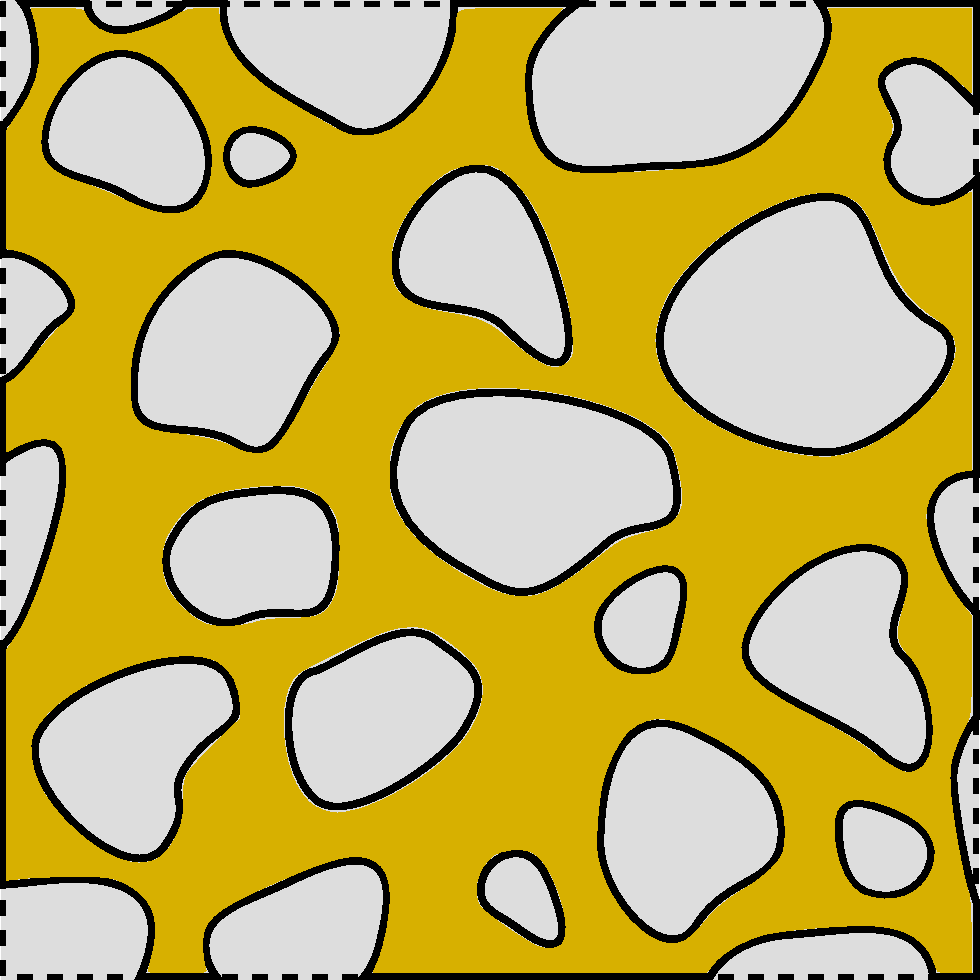
\includegraphics[scale=.3]{SwissCheeseFig}
   };
\draw[<-, line width=.4mm] (5.0,4.0) to[out=0,in=-120] (6.0,5.0) node[right=1pt,black]{$\Gamma_\rve^+$};
\draw[<-, line width=.4mm] (4.0,5.0) to[out=60,in=120] (6.0,5.0);
\draw[<-, line width=.4mm] (0.0,1.0) to[out=180,in=60] (-1.0,0.0) node[left=1pt,black]{$\Gamma_\rve^-$};
\draw[<-, line width=.4mm] (1.0,0.0) to[out=-120,in=-60] (-1.0,0.0);
\draw[<-, line width=.6mm] (0.0,2.4) to[out=15,in=165] (5.0,2.4) node[right]{$\ta{\varphi}_\per$} ;
%\draw[<-, line width=.4mm] (4.6,1.7) .. controls +(right:0.5cm) and +(left:0.5cm) .. (6.0,1.0) node[right=1pt,black,text width=3cm,text badly ragged]{$\partial\Omega_{\rve,i}^\text{p}$};
\end{tikzpicture}
\caption{SVE in 2D with ``image'' and ``mirror'' boundaries.}
\label{Figure2}
\end{figure}
%--------------------------------------------------------------------------------
In particular, we express micro-periodicity of the displacement fluctuation field as
%--------------------------------------------------------------------------------
\begin{equation}
    \ta{u}^\fluct(\ta{x}) = \ta{u}^\fluct(\ta{\varphi}_\per(\ta{x})), \quad
    \forall \ta{x}\in\Gamma_\rve^+
\label{eq21}
\end{equation}
%---------------------------------------------------------------------------
or, equivalently, in terms of the ``jump'' between the fluctuation fields on the image and mirror parts of the boundary as follows:
%--------------------------------------------------------------------------------
\begin{equation}
    \jmp{\ta{u}^\fluct} = \ta{0} \quad \makebox{on } \Gamma_\rve^+, \quad
    \jmp{\ta{u}^\fluct}(\ta{x}) \defeq \ta{u}^\fluct(\ta{x})-\ta{u}^\fluct(\ta{\varphi}_\per(\ta{x}))
\label{eq22}
\end{equation}
%---------------------------------------------------------------------------

Subsequently, we shall not enforce the condition \cref{eq22} strongly as the point of departure; rather it is done weakly.
To this end, we first assume that $\ts{\sigma}$ satisfies the \emph{symmetry condition}
%--------------------------------------------------------------------------------
\begin{equation}
    \ts{\sigma}(\ta{x}) = \ts{\sigma}(\ta{\varphi}_\per(\ta{x})), \quad
    \forall \ta{x}\in\Gamma_\rve^+
\label{eq23}
\end{equation}
%---------------------------------------------------------------------------
As an immediate consequence of this symmetry assumption, we obtain that the boundary tractions $\ta{t}\defeq\ts{\sigma}\cdot\ta{n}$ satisfy the following \emph{anti-symmetry condition} for any mirror point (that is not a corner point)
%--------------------------------------------------------------------------------
\begin{equation}
    \ta{t}(\ta{x}) = -\ta{t}(\ta{\varphi}_\per(\ta{x})), \quad
    \forall \ta{x}\in\Gamma_\rve^+
\label{eq24}
\end{equation}
%---------------------------------------------------------------------------
as depicted in \cref{Figure2}.
We now evaluate, upon using \cref{eq24}, the boundary term in
\cref{eq19a,eq20a}, as follows:
%----------------------------------------------------------------------------
\begin{equation}
    \int_{\Gamma_\rve} \ta{t} \cdot \delta \ta{u} \dif S =
    \int_{\Gamma_\rve^+} \ta{t} \cdot \jmp{\delta \ta{u}} \dif S
\label{eq25}
\end{equation}
%----------------------------------------------------------------------------

A weak statement of the micro-periodicity constraint, given in strong form in \cref{eq23}, is
%--------------------------------------------------------------------------------
\begin{equation}
    \frac{1}{\volume}\int_{\Gamma_\rve^+} \delta \ta{t} \cdot \jmp{\ta{u}^\fluct} \dif S = 0,
    \quad \forall \delta \ta{t}\in\set{T}_\rve
\label{eq26}
\end{equation}
%---------------------------------------------------------------------------
where the space of test functions that ``live'' only on the image boundary $\Gamma_\rve^+$ is given as:
%----------------------------------------------------------------------------
\begin{equation}
    \set{T}_\rve = \{\ta{t}\in [L_2(\Gamma_\rve^+)]^{3}\}
\label{eq25a}
\end{equation}
%----------------------------------------------------------------------------
Associated with this condition, we introduce the auxiliary variational form
%----------------------------------------------------------------------------
\begin{equation}
    d_\rve(\ta{t},\ta{u}) \defeq
    - \frac{1}{\volume}\int_{\Gamma_\rve^+} \ta{t} \cdot \jmp{\ta{u}} \dif S
\label{eq27}
\end{equation}
%----------------------------------------------------------------------------
whereby the constraint \cref{eq26} is expressed as
%----------------------------------------------------------------------------
\begin{equation}
    d_\rve(\delta\ta{t},\ta{u}^\fluct) = 0, \quad \forall \delta \ta{t}\in\set{T}_\rve
\label{eq27a}
\end{equation}
%----------------------------------------------------------------------------

\subsection{RVE-problem -- Original ``variationally consistent'' weak format}

In order to establish the most straightforward formulation of the RVE-problem, based on micro-periodicity, we introduce the following spaces for the fluctuation fields:
%----------------------------------------------------------------------------
\begin{align}
    \set{U}_\rve^\fluct &= \{\ta{v}\in [H^1(\Omega_\rve)]^{3} \,| \quad \frac{1}{|\Gamma_\rve|}\int_{\Gamma_\rve} \ta{v} \dif S = 0, \quad
    \frac{1}{\volume}\int_{\Omega_\rve} \ta{v}\outerp\diff \dif V = \ta{0} \}
\label{eq28a} \\
    \set{P}_\rve^\fluct &= \{q\in L_2(\Omega_\rve) \,| \quad \frac{1}{\volume}\int_{\Omega_\rve} q \dif V = 0 \}
\label{eq28b} \\
    \set{T}_\rve^\fluct &= \{\ta{s}\in [L_2(\Gamma_\rve^+)]^{3} \,| \quad \frac{1}{\volume}\int_{\Gamma_\rve^+} \ta{s}\outerp\jmp{\ta{x}-\bar{\ta{x}}} \dif S
    = \ta{0} \}
\label{eq28c}
\end{align}
%----------------------------------------------------------------------------
We remark, in particular, that $\set{T}_\rve^\fluct$ is restricted to such tractions that are self-equilibrating, i.e.\ they correspond to vanishing macroscale stress.
To show this, we first note that $\ta{x}(\ta{\varphi}_\per(\ta{x}))=-\ta{x}\,\,\forall \ta{x}\in\Gamma_\rve^+$, and we introduce the stress field $\ta{\sigma}'$ such that $\ta{t}'=\ts{\sigma}'\cdot\ta{n}\in\set{T}_\rve^\fluct$ and $\ta{\sigma}'\cdot\diff=\ta{0}$.
We then obtain
%----------------------------------------------------------------------------
\begin{align}
    \frac{1}{\volume}\int_{\Gamma_\rve^+} \ta{t}'\outerp\jmp{\ta{x}-\bar{\ta{x}}} \dif S = \frac{1}{\volume}\int_{\Gamma_\rve} \ta{t}'\outerp\ta{x} \dif S =
    \frac{1}{\volume}\int_{\Omega_\rve} \ts{\sigma}' \dif V  = \bar{\ts{\sigma}'} = \ta{0}
\label{eq28d}
\end{align}
%----------------------------------------------------------------------------

We are now in the position to establish the subscale problem:
For \emph{given} values $\bar{\ta{u}}$, $\bar{\ts{h}}$, and $\bar{p}$, that represent the macroscale fields (and which solve the macroscale problem), we first make the unique decomposition:
%----------------------------------------------------------------------------
\begin{subequations}\label{eq29}
\begin{alignat}{2}
    \ta{u} &= \bar{\ta{u}} + \bar{\ts{h}} \cdot [\ta{x}-\bar{\ta{x}}] + \ta{u}^\fluct, &\quad& \ta{u}^\fluct\in\set{U}_\rve^\fluct
\label{eq29a} \\
     p     &= \bar{p} + p^\fluct, &\quad& p^\fluct\in\set{P}_\rve^\fluct
\label{eq29b} \\
    \ta{t} &= \bar{\ts\tau}\cdot\ta{n} + \ta{t}^\fluct, &\quad& \bar{\ts\tau}\in\set{R}^{3\times 3},\,\,\ta{t}^\fluct\in\set{T}_\rve^\fluct
\label{eq29c}
\end{alignat}
\end{subequations}
%----------------------------------------------------------------------------
The unique decompositions are shown in \cref{appendix:unique_decomposition}.

%$\bar{\ts{h}}\defeq\bar{\ts\epsilon}_\dev+\frac{1}{3}\bar{e}\ts{I}+\bar{\ts{h}}^\skw$,
The motivation for the decomposition of tractions in \cref{eq29c} is the observation that
%----------------------------------------------------------------------------
\begin{equation}
    d_\rve(\bar{\ts{\tau}}\cdot\ts{n},\ta{u}^\fluct) = 0, \quad
    \forall \bar{\ts{\tau}}\in\set{R}^{3\times3}, \,\,\forall \ts{u}^\fluct\in\set{U}_\rve^\fluct
\label{eq27b}
\end{equation}
%----------------------------------------------------------------------------
Hence, \cref{eq27a} can be restricted to test functions in $\set{T}_\rve^\fluct$, and we note that the stress quantity $\bar{\ts\tau}$ is not part of the RVE-problem.
We shall also use the identity
%----------------------------------------------------------------------------
\begin{equation}
    b_\rve(\delta p^\fluct,\ta{u}) = b_\rve(\delta p^\fluct,\ta{u}^\fluct), \,\,\forall \delta p^\fluct\in\set{P}_\rve^\fluct
\label{eq27c}
\end{equation}
%----------------------------------------------------------------------------
whereby it is noted that the macroscale part of $\ta{u}$ is ``filtered out''.
As a consequence, the RVE-problem is reduced to finding the subscale fluctuations $(\ta{u}^\fluct,p^\fluct,\ta{t}^\fluct)\in\set{U}_\rve^\fluct\times\set{P}_\rve^\fluct\times\set{T}_\rve^\fluct$ that solve the system
%----------------------------------------------------------------------------
\begin{subequations}\label{eq31}
\begin{alignat}{3}
    a_\rve(\bar{\ts\epsilon}_\dev\cdot [\ta{x}-\bar{\ta{x}}]+\ta{u}^\fluct;\delta\ta{u}^\fluct) +
    b_\rve(\bar{p}+p^\fluct,\delta\ta{u}^\fluct) +
    d_\rve(\ta{t}^\fluct,\delta\ta{u}^\fluct) &= 0
    &\quad& \forall \delta\ta{u}^\fluct &&\in \set{U}_\rve^\fluct
\label{eq31a} \\
    b_\rve(\delta p^\fluct,\ta{u}^\fluct) + c^*_\rve(\bar{p}+p^\fluct;\delta p^\fluct) &= 0
    &\quad& \forall \delta p^\fluct &&\in \set{P}_\rve^\fluct
\label{eq31b} \\
    d_\rve(\delta\ta{t}^\fluct,\ta{u}^\fluct) &= 0
    &\quad& \forall \delta t^\fluct &&\in \set{T}_\rve^\fluct
\label{eq31c}
\end{alignat}
\end{subequations}
%----------------------------------------------------------------------------
where the SVE-functionals were introduced in \cref{eq8a,eq8b,eq8c,eq27}.
%%----------------------------------------------------------------------------
%\begin{eqnarray}
%    \frac{1}{\volume}\int_{\Omega_\rve} \ts{\epsilon}_\dev[\delta\ta{u}^\fluct]\dprod \hat{\ts{\sigma}}_\dev(\bar{\ts\epsilon}_\dev+\ts{\epsilon}_\dev[\ta{u}^\fluct]) \dif V
%    - \frac{1}{\volume}\int_{\Omega_\rve} [\bar{p}+p^\fluct] \delta\ta{u}^\fluct\cdot\diff \dif V &&
%\nonumber \\
%    - \frac{1}{\volume}\int_{\Gamma_\rve} \ta{t}^\fluct\cdot\jmp{\delta\ta{u}^\fluct} \dif S &=& 0
%    \quad \forall \delta\ta{u}^\fluct \in \set{U}_\rve^\fluct
%\label{eq31a} \\
%    - \frac{1}{\volume}\int_{\Omega_\rve} \delta p^\fluct\ta{u}^\fluct\cdot\diff \dif V
%    +  \frac{1}{\volume}\int_{\Omega_\rve} \delta p^\fluct\hat{e}(\bar{p}+p^\fluct) \dif V &=& 0
%    \quad \forall \delta p^\fluct \in \set{P}_\rve^\fluct
%\label{eq31b} \\
%   - \frac{1}{\volume}\int_{\Gamma_\rve^+} \delta\ta{t}^\fluct\cdot\jmp{\ta{u}^\fluct} \dif S &=& 0
%    \quad \forall \delta t^\fluct \in \set{T}_\rve^\fluct
%\label{eq31c}
%\end{eqnarray}
%%----------------------------------------------------------------------------

By inspecting the system in \cref{eq31}, we note that it is not the entire $\bar{\ts{h}}$ that is used as input to the RVE-problem.
In fact, it is readily concluded that it is only the deviatoric part $\bar{\ts\epsilon}_\dev=\bar{\ts{h}}^\sym_\dev$ that enters as ``data'' to the RVE-problem.
In other words, neither $\bar{\ta{u}}$, the volumetric part $\bar{h}_\vol\defeq\bar{\ts{h}}\dprod\ts{I}$, nor the skew-symmetric part $\bar{\ts{h}}^\skw=\frac{1}{2}[\bar{\ts{h}}-\bar{\ts{h}}^\majorT]$ will affect the SVE-solution.
In conclusion, ($\bar{\ts\epsilon}_\dev,\bar{p})$ are the macroscale variables that are used as data for the RVE-problem; hence, the solution of \cref{eq31} is parameterized as $\ta{u}^\fluct=\ta{u}^\fluct\{\bar{\ts\epsilon}_\dev,\bar{p}\}$, $p^\fluct=p^\fluct\{\bar{\ts\epsilon}_\dev,\bar{p}\}$, and $\ta{t}^\fluct=\ta{t}^\fluct\{\bar{\ts\epsilon}_\dev,\bar{p}\}$.
In a postprocessing step the homogenized ``fluxes'' can be represented as
%----------------------------------------------------------------------------------------------------------------
\begin{align}
    \bar{\ts\sigma}_\dev\{\bar{\ts\epsilon}_\dev,\bar{p}\} &\defeq
    \homgen{ \hat{\ts{\sigma}}_\dev(\ts{\epsilon}_\dev[\ta{u}]) } =
    \homgen{  \hat{\ts{\sigma}}_\dev(\bar{\ts\epsilon}_\dev + \ts{\epsilon}_\dev[\ta{u}^\fluct\{\bar{\ts\epsilon}_\dev,\bar{p}\}]) }
\label{eq33a} \\
    \bar{e}\{\bar{\ts\epsilon}_\dev,\bar{p}\} &\defeq
    \homgen{ \hat{e}(p) } =
    \homgen{ \hat{e}(\bar{p} + p^\fluct\{\bar{\ts\epsilon}_\dev,\bar{p}\}) }
\label{eq33b}
\end{align}
%---------------------------------------------------------------------------------------------------------------------
Note that $\bar{e}\{\bar{\ts\epsilon}_\dev,\bar{p}\}\neq\bar{h}_\vol$ in general!

From the aforesaid, it appears that there is a problem associated with the presented ``consistent'' format in the sense that the strong form of the continuity equation does not (necessarily) represent that one of the fine scale.
The reason is that the formulation \cref{eq31b} ``filters out'' any imposed \emph{constant} volumetric strain $\bar{\lambda}$; hence, the strong format generally reads
%----------------------------------------------------------------------------
\begin{equation}
    - \ta{u}\cdot\diff + \hat{e}(p) + \bar{\lambda} = 0, \quad \bar{\lambda}\in\set{R}
\label{eq34a}
\end{equation}
%----------------------------------------------------------------------------
Clearly, testing \cref{eq34a} with a constant pressure, we have $\bar{\lambda}=\bar{h}_\vol+\homgen{\ta{u}^\fluct\cdot\diff-\hat{e}(p)}$.

\textbf{Remark:} In the special case of intrinsically incompressible material response, defined by $\hat{e}(p)=0$ in $\Omega_\rve$, for any $p$, then we have  $\bar{\lambda}=\bar{h}_\vol+\homgen{\ta{u}^\fluct\cdot\diff}$.
However, from \cref{eq31b}, \cref{eq31c} it is concluded that the solution of the RVE-problem is $\ta{u}^\fluct\cdot\diff=0$ in $\Omega_\rve$, whereby we obtain $\bar{\lambda}=\bar{h}_\vol \neq 0$.
It is only when the macroscale solution represents incompressible response, i.e.\ when $\bar{h}_\vol = 0$, that we obtain $\bar{\lambda} = 0$.
In conclusion, the RVE-problem is able to provide an ``incompressible solution'' even in the case that the macroscale solution represents compressible response.
This anomaly is the main motivation for establishing an alternative format of the problem, which is discussed next. $\Box$

\todo{fix}
Macro-homogeneity condition satisfied, since $R(\bullet;\delta\ta u^\fluct, \delta p^\fluct, \delta\ta t^\fluct) = 0$.

%\subsection{RVE-problem -- Consistent weak format of type I}
%
%A generalized formulation of the RVE-problem that does not contain the above-mentioned inconsistency with the strong format is considered next.
%We then introduce the following spaces for the total (macroscale and fluctuation) fields:
%%----------------------------------------------------------------------------
%\begin{eqnarray}
%    \set{U}_\rve &=& \{\ta{v}\in [H^1(\Omega_\rve)]^{3} \,|\,\, \frac{1}{\volume}\int_{\Gamma_\rve} \ta{v} \dif S = \ta{0} \}
%\label{eq35a} \\
%    \set{P}_\rve &=& \{q\in L_2(\Omega_\rve) \}
%\label{eq35b} \\
%    \set{T}_\rve' &=& \{\ta{s}\in [L_2(\Gamma_\rve^+)]^{3} \,|\,\, \frac{1}{\volume}\int_{\Gamma_\rve^+} \ta{s}\cdot\jmp{\ta{x}_\mean} \dif S
%    = 0 \}
%\label{eq35c}
%\end{eqnarray}
%%----------------------------------------------------------------------------
%where $\ta{x}_\mean\defeq\frac{1}{3}\ta{x}-\bar{\ta{x}}$.
%We remark, in particular, that $\set{T}_\rve'$ is restricted to such tractions that equilibrate purely deviator stresses, i.e.\ they are in equilibrium with stresses within $\Omega_\rve$ that must not contain an arbitrary???? spherical component.
%
%We are now in the position to establish the alternative formulation of the subscale problem: For given values $\bar{\ts\epsilon}_\dev, \bar{p}$, that represent the macroscale solution, find the subscale fields $\tilde{\ta{u}},\tilde{p},\tilde{\ta{t}}\in\set{U}_\rve\times\set{P}_\rve\times\set{T}_\rve'$ that solve the system
%%----------------------------------------------------------------------------
%\begin{eqnarray}
%    \frac{1}{\volume}\int_{\Omega_\rve} \ts{\epsilon}_\dev[\delta\tilde{\ta{u}}]\dprod \hat{\ts{\sigma}}_\dev(\ts{\epsilon}_\dev[\tilde{\ta{u}}])
%    \dif V  - \frac{1}{\volume}\int_{\Omega_\rve^+} \tilde{p}\delta\tilde{\ta{u}}\cdot\diff \dif V &&
%\nonumber \\
%    - \frac{1}{\volume}\int_{\Gamma_\rve} \tilde{\ta{t}}\cdot\jmp{\delta\tilde{\ta{u}}} \dif S &=&
%    - \bar{p} \left[\frac{1}{\volume}\int_{\Omega_\rve} \delta\tilde{\ta{u}}\cdot\diff \dif V\right]
%    \quad \forall \delta\tilde{\ta{u}} \in \set{U}_\rve
%\label{eq36a} \\
%    - \frac{1}{\volume}\int_{\Omega_\rve} \delta \tilde{p}\tilde{\ta{u}}\cdot\diff \dif V
%    +  \frac{1}{\volume}\int_{\Omega_\rve} \delta \tilde{p}\hat{e}(\tilde{p}) \dif V &=& 0
%    \quad \forall \delta \tilde{p} \in \set{P}_\rve
%\label{eq37b} \\
%   - \frac{1}{\volume}\int_{\Gamma_\rve^+} \delta\tilde{\ta{t}}\cdot\jmp{\tilde{\ta{u}}} \dif S &=&
%    - \bar{\ts\epsilon}_\dev \dprod \left[\frac{1}{\volume}\int_{\Gamma_\rve^+} \delta\tilde{\ta{t}}\outerp\jmp{\ta{x}-\bar{\ta{x}}} \dif S\right]
%    \quad \forall \delta \tilde{p} \in \set{T}_\rve'
%\label{eq38c}
%\end{eqnarray}
%%----------------------------------------------------------------------------
% ANALYSIS?
% %----------------------------------------------------------------------------
% \begin{eqnarray}
%    \tilde{\ta{u}}\{\bar{\ts\epsilon}_\dev,\bar{p}\} &=& \bar{\ts\epsilon}_\dev\cdot[\ta{x}-\bar{\ta{x}}] +
%    \tilde{\bar{\epsilon}}_\vol\ta{x}_\mean + \tilde{\ta{u}}^\fluct\{\bar{\ts\epsilon}_\dev,\bar{p}\} \quad
% \label{eq40a} \\
%     \tilde{p}\{\bar{\ts\epsilon}_\dev,\bar{p}\} &=& \bar{p} + \tilde{p}^\fluct\{\bar{\ts\epsilon}_\dev,\bar{p}\} \quad
% \label{eq40b} \\
%    \tilde{\ta{t}}\{\bar{\ts\epsilon}_\dev,\bar{p}\} &=& \left[\tilde{\bar{\ts\sigma}}_\dev + \tilde{\bar{\ts\sigma}}^\skw\right]\cdot\ta{n} +
%    \tilde{\ta{t}}^\fluct\{\bar{\ts\epsilon}_\dev,\bar{p}\}
% \label{eq40c}
% \end{eqnarray}
%%----------------------------------------------------------------------------
%From \cref{eq16}, we may then conclude that the homogenized ``fluxes'' can be represented as
%%----------------------------------------------------------------------------------------------------------------
%\begin{eqnarray}
%    \bar{\ts\sigma}_\dev\{\bar{\ts\epsilon}_\dev,\bar{p}\} &\defeq&
%    \homgen{ \hat{\ts{\sigma}}_\dev(\ts{\epsilon}_\dev[\tilde{\ta{u}}]) }
%\label{eq41a} \\
%    \bar{e}\{\bar{\ts\epsilon}_\dev,\bar{p}\} &\defeq&
%    \homgen{ \hat{e}(\tilde{p}) }
%\label{eq41b}
%\end{eqnarray}
%%---------------------------------------------------------------------------------------------------------------------


\subsection{RVE-problem -- Canonical weak format}

A generalized formulation of the RVE-problem that does not contain the above-mentioned inconsistency with the strong format is considered next.
Firstly, we introduce the following spaces for the total (macroscale and fluctuation) fields:
%----------------------------------------------------------------------------
\begin{align}
    \set{U}_\rve &= \{\ta{v}\in [H^1(\Omega_\rve)]^{3} \,| \quad \frac{1}{\volume}\int_{\Gamma_\rve} \ta{v} \dif S = \ta{0} \}
\label{eq45a} \\
    \set{P}_\rve &= \{q\in L_2(\Omega_\rve) \}
\label{eq45b} \\
    \set{T}_\rve &= \{\ta{s}\in [L_2(\Gamma_\rve^+)]^{3} \}
\label{eq45c}
\end{align}
%----------------------------------------------------------------------------
Secondly, the fine-scale fields within an RVE are decomposed as
%----------------------------------------------------------------------------
\begin{subequations}\label{eq129}
\begin{alignat}{2}
    \ta{u} &= \bar{\ts\epsilon}_\dev \cdot [\ta{x}-\bar{\ta{x}}] + \bar{e}\,\ta{x}_\mean + \ta{u}^\fluct, &\quad& \ta{u}^\fluct\in\set{U}_\rve^\fluct
\label{eq129a} \\
     p     &= \bar{p} + p^\fluct, &\quad& p^\fluct\in\set{P}_\rve^\fluct
\label{eq129b}
\end{alignat}
\end{subequations}
%----------------------------------------------------------------------------
where $\ta{x}_\mean\defeq\frac{1}{3}[\ta{x}-\bar{\ta{x}}]$, and where $\bar{e}$ is an additional scalar quantity which, at the outset, does not depend on the macroscale field(s).

We are now in the position to establish the alternative, subsequently denoted \emph{canonical}, formulation of the RVE-problem as follows: For given values $\bar{\ts\epsilon}_\dev$, $ \bar{p}$, that represent the macroscale fields (which solve the macroscale problem), find the subscale fields ($\ta{u},p,\ta{t},\bar{e})\in\set{U}_\rve\times\set{P}_\rve\times\set{T}_\rve\times\set{R}$ that solve the system
%%----------------------------------------------------------------------------
%\begin{alignat}{2}
%    \tilde{\ta{u}} &= \tilde{\bar{\ta{u}}} + \bar{\ts\epsilon}_\dev\cdot[\ta{x}-\bar{\ta{x}}] + \bar{e}\,\ta{x}_\mean + \tilde{\ta{u}}^\fluct, &\quad& \bar{e}\in \set{R}, \,\,\tilde{\ta{u}}^\fluct\in\set{U}_\rve^\fluct
%\label{eq47a} \\
%     \tilde{p}     &= \tilde{\bar{p}} + \tilde{p}^\fluct, &\quad& \tilde{\bar{p}}\in\set{R}, \,\,\tilde{p}^\fluct\in\set{P}_\rve^\fluct
%\label{eq47b} \\
%    \tilde{\ta{t}} &= \tilde{\bar{\ts\tau}}\cdot\ta{n} + \tilde{\ta{t}}^\fluct, &\quad& \tilde{\bar{\ts\tau}}\in\set{R}^{3\times 3},\,\,\tilde{\ta{t}}^\fluct\in\set{T}_\rve^\fluct
%\label{eq47c}
%\end{alignat}
%%----------------------------------------------------------------------------
%----------------------------------------------------------------------------
\begin{subequations}\label{eq51}
\begin{alignat}{3}
    a_\rve(\ta{u};\delta\ta{u}) + b_\rve(p,\delta\ta{u}) + d_\rve(\ta{t},\delta\ta{u}) &= 0
    &\quad& \forall \delta\ta{u} &&\in \set{U}_\rve
\label{eq51a} \\
    b_\rve(\delta p,\ta{u}) + c^*_\rve(p;\delta p) &= 0
    &\quad& \forall \delta p &&\in \set{P}_\rve
\label{eq51b} \\
    d_\rve(\delta\ta{t},\ta{u}) - d_\rve(\delta\ta{t},\bar{e}\,\ta{x}_\mean) &= d_\rve(\delta\ta{t},\bar{\ts\epsilon}_\dev \cdot[\ta{x}-\bar{\ta{x}}])
    &\quad& \forall \delta\ta{t} &&\in \set{T}_\rve
\label{eq51c} \\
    - d_\rve(\ta{t},\delta\bar{e}\,\ta{x}_\mean) &=
    - \bar{p}\,\delta\bar{e}
    &\quad& \forall \delta\bar{e} &&\in \set{R}
\label{eq51d}
\end{alignat}
\end{subequations}
%----------------------------------------------------------------------------
It follows from \cref{eq51} that the variable $\bar{e}$ still obtains the value $\bar{e} = \homgen{\hat{e}(p)}$.
To show this result, we first use the divergence theorem to obtain the identities
%--------------------------------------------------------------------------------------------------------
\begin{align}
    -b_\rve(1, \bullet) &= d_\rve(\ta n, \bullet), \quad  d_\rve(\ta n, \ta x_\mean) = -b_\rve(1, \ta x_\mean) =  1
\end{align}
%----------------------------------------------------------------------------------------------------------
Using these identities together with \cref{eq51b}, \cref{eq51c}, we deduce
%--------------------------------------------------------------------------------------------------------
\begin{multline}
 \homgen{\hat{e}(p)} = c_\rve^*(p; 1) = -b_\rve(1, \ta u) = d_\rve(\ta n, \ta u) = \bar{e}\;d_\rve(\ta n, \ta x_\mean) + d_\rve(\ta{n}, \bar{\ts\epsilon}_\dev \cdot[\ta{x}-\bar{\ta{x}}]) 
\\
= - \bar{e}\,b_\rve(1, \ta x_\mean) + \frac{1}{\volume}\int_{\Gamma_\rve^+} \ta n \outerp \jmp{\ta x - \bar{\ta x}}\dif S \dprod \bar{\ts\epsilon}_\dev 
= \bar{e} + \ts I \dprod \bar{\ts\epsilon}_\dev = \bar{e}.
\end{multline}



%----------------------------------------------------------------------------------------------------------
% \textbf{Remark}: The new variable $\bar{e}$, which represents the volumetric strain, is not necessarily identical to the macroscopic volumetric strain $\bar{h}_\vol=\bar{\ts{h}}\dprod\ts{I}=\bar{\ta{u}}\cdot\diff$.
%
% The (auxiliary) macroscale stress $\bar{\ts\tau}$ and the macroscale deformation gradient $\bar{\ts{h}}$ can be expressed as
% %----------------------------------------------------------------------------------------------------------------
% \begin{subequations}
% \begin{alignat}{2}
%     \bar{\ts\tau}\{\bar{\ts\epsilon}_\dev,\bar{p}\} = \bar{\ts\sigma}_\dev\{\bar{\ts\epsilon}_\dev,\bar{p}\} - \bar{p}\ts{I} &\quad\text{ with }\quad&&
%     \bar{\ts\sigma}_\dev\{\bar{\ts\epsilon}_\dev,\bar{p}\} \defeq
%     \homgen{ \hat{\ts{\sigma}}_\dev(\ts{\epsilon}_\dev[\ta{u}\{\bar{\ts\epsilon}_\dev,\bar{p}\}]) }
% \label{eq53a} \\
%     \bar{\ts{h}}\{\bar{\ts\epsilon}_\dev,\bar{p}\} = \bar{\ts\epsilon}_\dev + \frac{1}{3}\bar{e}\{\bar{\ts\epsilon}_\dev,\bar{p}\}\ts{I} &\quad\text{ with }\quad&&
%     \bar{e}\{\bar{\ts\epsilon}_\dev,\bar{p}\} \defeq
%     \homgen{ \hat{e}(p\{\bar{\ts\epsilon}_\dev,\bar{p}\}) }
% \label{eq53b}
% \end{alignat}
% \end{subequations}
%---------------------------------------------------------------------------------------------------------------------
The solution of the ``canonical'' problem \cref{eq51} contains, in fact, the solution of the original ``variationally consistent'' problem in \cref{eq31}; however, without the apparent drawback that is associated with that format.
The fluctuations
%----------------------------------------------------------------------------
\begin{subequations}
\begin{align}
    \ta u^\fluct\{\bar{\ts\epsilon}_\dev, \bar{p}\} &= \ta u\{\bar{\ts\epsilon}_\dev, \bar{p}\} - \bar{\ts\epsilon}_\dev \cdot[\ta x - \bar{\ta x}] - \bar{e}\{\bar{\ts\epsilon}_\dev, \bar{p}\}\,\ta x_\mean
\label{eq52a} \\
    p^\fluct\{\bar{\ts\epsilon}_\dev, \bar{p}\} &= p\{\bar{\ts\epsilon}_\dev, \bar{p}\} - \bar{p}
\label{eq52b} \\
    \ta t^\fluct\{\bar{\ts\epsilon}_\dev, \bar{p}\} &= \ta t\{\bar{\ts\epsilon}_\dev, \bar{p}\} - [\bar{\ts\sigma}_\dev\{\bar{\ts\epsilon}_\dev, \bar{p}\} - \bar{p}\ts I]\cdot \ta n
\label{eq52c}
\end{align}
\end{subequations}
% \begin{align}
%     \ta{u}\{\bar{\ts\epsilon}_\dev,\bar{p}\} &= \bar{\ts\epsilon}_\dev\cdot[\ta{x}-\bar{\ta{x}}] +
%     \bar{e}\{\bar{\ts\epsilon}_\dev,\bar{p}\}\ta{x}_\mean + \ta{u}^\fluct\{\bar{\ts\epsilon}_\dev,\bar{p}\}
% \label{eq52a} \\
%      p\{\bar{\ts\epsilon}_\dev,\bar{p}\} &= \bar{p} + p^\fluct\{\bar{\ts\epsilon}_\dev,\bar{p}\}
% \label{eq52b} \\
%     \ta{t}\{\bar{\ts\epsilon}_\dev,\bar{p}\} &= \left[\bar{\ts\sigma}_\dev\{\bar{\ts\epsilon}_\dev,\bar{p}\} - \bar{p}\ts{I}\right]\cdot\ta{n} +  \ta{t}^\fluct\{\bar{\ts\epsilon}_\dev,\bar{p}\}
% \label{eq52c}
% \end{align}
%----------------------------------------------------------------------------
can be shown to be identical to ($\ta{u}^\fluct,p^\fluct,\ta{t}^\fluct)\in\set{U}_\rve^\fluct\times\set{P}_\rve^\fluct\times\set{T}_\rve^\fluct$ that solve the system \cref{eq31}.
Since the macroscopic response variables are identical, VCMC is still fulfilled.

\begin{figure}[!htpb]
 \centering
 %h = rand(2)*0.5; hsym = 0.5*(h + h'); hsymdev = hsym - mean(diag(hsym))*eye(2);
%u1 = h*c; u2 = hsymdev*c; c1 = c+u1; c2 = c+u2;
%all = [1:4,1]
%plot(c(1,all), c(2,all), '--', c1(1,all), c1(2,all), 'b-', c2(1,all), c2(2,all), 'r-')
%printf("(%f, %f) -- ", c1(:,all))
%printf("(%f, %f) -- ", c2(:,all))

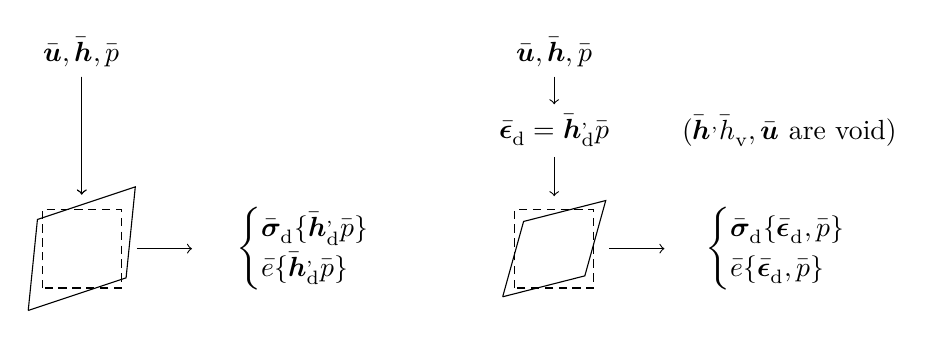
\begin{tikzpicture}[]
 \node (D) at (0,2.5) {$\bar{\ta u}, \bar{\ts h}, \bar p$};
 \draw[densely dashed] (-0.5,-0.5) rectangle (0.5,0.5);
 \draw[] (-0.679901, -0.785203) -- (0.562857, -0.370962) -- (0.679901, 0.785203) -- (-0.562857, 0.370962) -- (-0.679901, -0.785203);
 \node at (3,0) {$\begin{cases} \bar{\ts\sigma}_\dev\{\bar{\ts h}_\dev^\sym, \bar{p}\} \\ \bar{e}\{\bar{\ts h}_\dev^\sym, \bar{p}\}\end{cases}$};
 \draw[->] (D.south) -- +(0,-1.5);
 \draw[->] (D.south) -- +(0,-1.5);
 \draw[->] (0.7,0) -- (1.4,0);

 \begin{scope}[shift={(6,0)}]
 \draw[densely dashed] (-0.5,-0.5) rectangle (0.5,0.5);
 \draw[] (-0.654469, -0.611173) -- (0.388827, -0.345531) -- (0.654469, 0.611173) -- (-0.388827, 0.345531) -- (-0.654469, -0.611173);
 \node (A) at (0,2.5) {$\bar{\ta u}, \bar{\ts h}, \bar p$};
 \node (B) at (0,1.5) {$\bar{\ts \epsilon}_\dev = \bar{\ts h}_\dev^\sym, \bar{p}$};
 \node[anchor=west] at (1.5,1.5) {($\bar{\ts h}^\skw, \bar{h}_\vol, \bar{\ta u}$ are void)};
 \node at (3,0) {$\begin{cases} \bar{\ts\sigma}_\dev\{\bar{\ts\epsilon}_\dev, \bar{p}\} \\ \bar{e}\{\bar{\ts\epsilon}_\dev, \bar{p}\}\end{cases}$};
 \draw[->] (A.south) -- (B.north);
 \draw[->] (B.south) -- +(0,-0.5);
 \draw[->] (0.7,0) -- (1.4,0);
 \end{scope}
 
\end{tikzpicture}
 \caption{Comparison of the original (left) and new RVE-problem formulation (right).}\label{fig:format_comparison}
\end{figure}
An illustrative comparison between the two RVE formulations are shown \cref{fig:format_comparison}.
Despite the different displacement fields, the homogenized responses, $\bar{\ts\sigma}_\dev$ and $\bar{e}$, are the same.

\subsection{RVE-problem -- Canonical weak format in the incompressible limit}

Fine-scale incompressibility within the RVE is defined by $\hat{e}(p)=0 \,\,\forall \ta{x}\in\Omega_\rve$, which gives  $c^*_\rve(p;\delta p)=0\,\,\forall\delta p \in \set{P}_\rve$.
As a result, $\bar{e}\{\bar{\ts\epsilon}_\dev,\bar{p}\}=\homgen{ \hat{e}(p) }=0$, and we obtain the reduced RVE-problem: For given values $\bar{\ts\epsilon}_\dev$, $ \bar{p}$, that represent the macroscale fields, find the subscale fields $(\ta{u},p,\ta{t})\in\set{U}_\rve\times\set{P}_\rve\times\set{T}_\rve$ that solve the system
%----------------------------------------------------------------------------
\begin{subequations}\label{eq251}
\begin{alignat}{3}
    a_\rve(\ta{u},\delta\ta{u}) + b_\rve(p,\delta\ta{u}) + d_\rve(\ta{t},\delta\ta{u}) &= 0
    &\quad& \forall \delta\ta{u} &&\in \set{U}_\rve
\label{eq251a} \\
    b_\rve(\delta p,\ta{u}) &= 0
    &\quad& \forall \delta p &&\in \set{P}_\rve
\label{eq251b} \\
    d_\rve(\delta\ta{t},\ta{u}) &= d_\rve(\delta\ta{t},\bar{\ts\epsilon}_\dev \cdot[\ta{x}-\bar{\ta{x}}])
    &\quad& \forall \delta\ta{t} &&\in \set{T}_\rve
\label{eq251c}
%    - d_\rve(\ta{t},\delta\bar{e}\,\ta{x}_\mean) &=
%    - \bar{p}\,\delta\bar{e}
%    &\quad& \forall \delta\bar{e} &&\in \set{R}
%\label{eq251d}
\end{alignat}
\end{subequations}
%----------------------------------------------------------------------------
In practice, there is (of course) no need to establish \cref{eq251} as a separate system from \cref{eq51}, since $\bar{e}=0$ is obtained directly as part of the solution of \cref{eq51} in this case.

%\section{Special cases of the RVE-problem: Dirichlet and Neumann boundary conditions}
%
%\subsection{Weak format for Dirichlet boundary conditions}
%
%%In order to establish a suitable variational setting we introduce the solution space $\set{U}_\rve^\Dirichlet\subseteq\set{U}_\rve$ and test space $\set{U}_\rve^{\Dirichlet,0}$
%%%----------------------------------------------------------------------------
%%\begin{align}
%%    \set{U}_\rve^\Dirichlet &= \{\ta{v}\in \set{U}_\rve \,|\,\, \exists\tilde{\bar{\ts\epsilon}}_\dev,\tilde{\bar{e}}\in\set{R}^{3\times3}_\dev \times\set{R} \text{ s.t. }
%%    \ta{v}=\tilde{\bar{\ts\epsilon}}_\dev\cdot[\ta{x}-\bar{\ta{x}}]+\tilde{\bar{e}}\,\ta{x}_\mean+\ta{v}^\fluct \text{ with } \ta{v}^\fluct=\ta{0} \text{ on } \Gamma_\rve \}
%%\label{eq61a} \\
%%    \set{U}_\rve^{\Dirichlet,0} &= \{\ta{v}\in \set{U}_\rve \,|\,\, \ta{v}=\ta{0} \text{ on } \Gamma_\rve \}
%%\label{eq61b}
%%\end{align}
%%%----------------------------------------------------------------------------
%%while $\set{P}_\rve^\Dirichlet=\set{P}_\rve$, ${\set{T}}_\rve^\Dirichlet={\set{T}}_\rve$ are the same spaces as for the generic problem.
%
%Upon inserting the \emph{ansatz} for $\ta{u}\in\set{U}_\rve^\Dirichlet$ into \cref{eq51c}, we obtain the identities
%%----------------------------------------------------------------------------
%\begin{equation}
%    \tilde{\bar{\ts\epsilon}}_\dev = \bar{\ts\epsilon}_\dev, \quad \tilde{\bar{e}} = \bar{e}
%\label{eq63}
%\end{equation}
%%----------------------------------------------------------------------------
%We also note that $d_\rve(\ta{t},\delta\ta{u}^\fluct)=0$ for any traction $\ta{t}$ and any choice of test function $\delta\ta{u}^\fluct\in\set{U}_\rve^{\Dirichlet,0}$.
%As a result, $\ta{t}$ will remain as a variable only in \cref{eq51d}, which can be replaced by an equation that does not contain $\ta{t}$: Choose $\delta\ta{u}=\delta\bar{e}\,\ta{x}_\mean$ in \cref{eq51a}, which then becomes
%%----------------------------------------------------------------------------
%\begin{equation}
%    \underbrace{a_\rve(\ta{u},\delta\bar{e}\,\ta{x}_\mean)}_{=0} + b_\rve(p,\delta\bar{e}\,\ta{x}_\mean) + d_\rve(\ta{t},\delta\bar{e}\,\ta{x}_\mean) = 0
%\label{eq63a}
%\end{equation}
%%----------------------------------------------------------------------------
%Combining this result with \cref{eq51d}, we obtain the (equivalent) equation
%%----------------------------------------------------------------------------
%\begin{equation}
%    b_\rve(p,\delta\bar{e}\,\ta{x}_\mean) = - \bar{p}\delta\bar{e} \quad \forall\delta\bar{e}\in\set{R} \,\,\Leftrightarrow\,\,
%    \homgen{ p } = \bar{p}
%\label{eq63b}
%\end{equation}
%%----------------------------------------------------------------------------
%In order to obtain \cref{eq63b}$_2$, we used the identity $\ta{x}_\mean\cdot\diff=1$.
%
%%We may now establish the RVE-problem subjected to Dirichlet boundary conditions as follows:
%%For given values $\bar{\ts\epsilon}_\dev, \bar{p}$, find the subscale fields $\ta{u}^\fluct,p,\bar{e}\in\set{U}_\rve^{\Dirichlet,0}\times\set{P}_\rve\times\set{R}$ that solve the system
%%%----------------------------------------------------------------------------
%%\begin{subequations}
%%\begin{alignat}{3}
%%    a_\rve(\bar{\ts\epsilon}_\dev\cdot[\ta{x}-\bar{\ta{x}}]+\ta{u}^\fluct,\delta\ta{u}^\fluct) + b_\rve(p,\delta\ta{u}^\fluct) &= 0
%%    &\quad& \forall \delta\ta{u}^\fluct &&\in \set{U}_\rve^{\Dirichlet,0}
%%\label{eq64a} \\
%%    b_\rve(\delta p,\ta{u}^\fluct) + b_\rve(\delta p,\bar{e}\,\ta{x}_\mean) + c^*_\rve(p;\delta p) &= 0
%%    &\quad& \forall \delta p &&\in \set{P}_\rve
%%\label{eq64b} \\
%%    b_\rve(p,\delta\bar{e}\,\ta{x}_\mean) &=
%%    - \bar{p}\,\delta\bar{e}
%%    &\quad& \forall \delta\bar{e} &&\in \set{R}
%%\label{eq64c}
%%\end{alignat}
%%\end{subequations}
%%%----------------------------------------------------------------------------
%
%%\subsection{Macroscale ATS-tensor}
%
%\subsection{Weak format for Neumann boundary conditions}
%
%%The problem defined by Neumann boundary conditions is obtained from the
%%general format upon restricting the space $\set{T}_\rve$, i.e.
%%introducing $\set{T}_\rve^\Neumann\subseteq\set{T}_\rve$ defined as
%%%----------------------------------------------------------------------------
%%\begin{equation}
%%    \set{T}_\rve^\Neumann =
%%    \{\ta{t}\in\set{T}_\rve\,|\,\, \exists\tilde{\bar{\ts\sigma}}_\dev,\tilde{\bar{p}}\in\set{R}^{3\times3}_\dev \times\set{R} \text{ s.t. }
%%    \ta{t}=\left[\tilde{\bar{\ts\sigma}}_\dev-\tilde{\bar{p}}\ts{I}\right]\cdot\ta{n} \text{ on } \Gamma_\rve^+\}
%%    \label{eq65}
%%\end{equation}
%%%---------------------------------------------------------------------------
%%while $\set{U}_\rve^\Neumann=\set{U}_\rve$ and $\set{P}_\rve^\Neumann=\set{P}_\rve$ are left unrestricted.
%Clearly, the choice of $\set{T}_\rve^\Neumann$ restricts the tractions to become piecewise constant on each of the three positive boundary faces of the SVE-cube.
%
%Firstly, upon inserting the \emph{ansatz} for $\ta{t}\in\set{T}_\rve^\Neumann$ into \cref{eq51d}, we directly obtain the identity $\tilde{\bar{p}}=\bar{p}$.
%Secondly, we introduce the auxiliary variational form $d'_\rve$ via the identity
%%----------------------------------------------------------------------------
%\begin{equation}
%    d'_\rve(\bar{\ts\tau},\ta{v}) \defeq  d_\rve(\bar{\ts\tau}\cdot\ta{n},\ta{v}) =
%%    \hat{\bar{\ts\tau}} : \homgen{ \ts{\epsilon} }
%    - \bar{\ts\tau} : \frac{1}{\volume}\int_{\Gamma_\rve^+} \jmp{\ta{v}}\outerp\ta{n} \dif S
%\label{eq66}
%\end{equation}
%%----------------------------------------------------------------------------
%for $\bar{\ts\tau}\in\set{R}^{3\times3}$.
%%We may now establish the RVE-problem subjected to Neumann boundary conditions as follows:
%%For given values $\bar{\ts\epsilon}_\dev, \bar{p}$, find the subscale fields $\ta{u},p,\tilde{\bar{\ts\sigma}}_\dev\in\set{U}_\rve\times\set{P}_\rve\times\set{R}^{3\times 3}_\dev$ that solve the system
%%%----------------------------------------------------------------------------
%%\begin{subequations}\label{eq67}
%%\begin{alignat}{3}
%%    a_\rve(\ta{u},\delta\ta{u}) + b_\rve(p,\delta\ta{u}) +  d'_\rve(\tilde{\bar{\ts\sigma}}_\dev,\delta\ta{u}) &= \bar{p}\,d'_\rve(\ts{I},\delta\ta{u})
%%    & \quad & \forall \delta\ta{u} &&\in \set{U}_\rve
%%\label{eq67a} \\
%%    b_\rve(\delta p,\ta{u}) + c^*_\rve(p;\delta p) &= 0
%%    & \quad & \forall \delta p &&\in \set{P}_\rve
%%\label{eq67b} \\
%%    d'_\rve(\delta\tilde{\bar{\ts\sigma}}_\dev,\ta{u}) &= - \bar{\ts\epsilon}_\dev\dprod\delta\tilde{\bar{\ts\sigma}}_\dev
%%    & \quad & \forall \delta\tilde{\bar{\ts\sigma}}_\dev &&\in\set{R}^{3\times3}_\dev
%%\label{eq67c}
%%\end{alignat}
%%\end{subequations}
%%%----------------------------------------------------------------------------
%We remark that \cref{eq67c} was obtained upon testing \cref{eq51c}$_1$ with $\tilde{\delta\ta{t}}=\delta\tilde{\bar{\ts\sigma}}_\dev\cdot\ta{n}$ for all possible $\delta\tilde{\bar{\ts\sigma}}_\dev\in\set{R}^{3\times 3}_\dev$.
%Moreover, we note that
%%----------------------------------------------------------------------------
%\begin{equation}
%    d'_\rve(\ts{I},\delta\ta{u}) = - \frac{1}{\volume}\int_{\Gamma_\rve^+} \jmp{\delta\ta{u}}\outerp\ta{n} \dif S =
%    \homgen{\delta\ta{u}\cdot\diff }
%\label{eq68}
%\end{equation}
%%---------------------------------------------------------------------------
%In a post-processing step, we may test \cref{eq67}$_1$ with $\delta\ta{u}=\delta\tilde{\bar{\ts\epsilon}}_\dev\cdot[\ta{x}-\bar{\ta{x}}]$ for all possible $\delta\tilde{\bar{\ts\epsilon}}_\dev\in\set{R}^{3\times 3}_\dev$ to identify the value $\tilde{\bar{\ts\sigma}}_\dev$ as the ``flux'' variable already defined in \cref{eq53a}.
%Moreover, testing \cref{eq51c}$_1$ with $\delta\tilde{\ta{t}}=\delta\tilde{\bar{p}}\,\ta{n}$ for all possible $\delta\tilde{\bar{p}}\in\set{R}$, we obtain the homogenized flux $\bar{e}$.
%In conclusion,
%%----------------------------------------------------------------------------------------------------------------
%\begin{align}
%    \tilde{\bar{\ts\sigma}}_\dev\{\bar{\ts\epsilon}_\dev,\bar{p}\} &= \bar{\ts\sigma}_\dev\{\bar{\ts\epsilon}_\dev,\bar{p}\} \,\,\text{ with }\,\,
%    \bar{\ts\sigma}_\dev\{\bar{\ts\epsilon}_\dev,\bar{p}\} \defeq
%    \homgen{ \hat{\ts{\sigma}}_\dev(\ts{\epsilon}_\dev[\tilde{\ta{u}}]) }
%\label{eq72a} \\
%    \bar{e}\{\bar{\ts\epsilon}_\dev,\bar{p}\} &= d'_\rve(\ts{I},\ta{u}\{\bar{\ts\epsilon}_\dev,\bar{p}\}) = \homgen{ \ta{u}\{\bar{\ts\epsilon}_\dev,\bar{p}\}\cdot\diff }
%\label{eq72b}
%\end{align}
%%---------------------------------------------------------------------------------------------------------------------
%

%
%\textbf{UPDATE} XXXXXXXXXXXXXXXXXXXXXXXXXXXXXXX
%
%The VCMC is satisfied, which is shown as follows: Consider the sensitivity $\dif\ta{u}^\fluct\in{\set{U}}_\rve^\Neumann$ for a perturbation $\dif \ta{u}^\macro$ of the macroscale field.
%From the conditions in \cref{eq22} it then follows that $\bar{\ta{u}}_\rve(\ta{u}^\fluct)=\ta{0}$ and $\bar{\ts\epsilon}_\rve(\ta{u}^\fluct)=\ta{0}$; hence we obtain directly from \cref{eq31a} that
%%----------------------------------------------------------------------------------------------------------------
%\begin{equation}
%    a_\rve(\ta{u},\dif \ta{u}^\fluct)
%    = 0 \quad \forall \dif \ta{u}^\macro \in \set{U}^{\macro,0}
%\label{eq133}
%\end{equation}
%%----------------------------------------------------------------------------------------------------------------------
%which is precisely the VCMC stated in \cref{eq10}.
%


\section{Variational properties of the RVE-problem -- Energy bounds from SVE-functional}

\subsection{Variational properties for the canonical formulation of the RVE-problem -- The RVE-potential}

In order to establish bounds on the effective properties based on the results from the Dirichlet and Neumann problems, we shall introduce an appropriate ``SVE-potential'' as follows:
%----------------------------------------------------------------------------------------------------------------
\begin{equation}
    \Pi_\rve(\bar{\ts\epsilon}_\dev,\bar{p};\ta{u},p,\ta{t},\bar{e}) =
    \Lambda_\rve(\ta{u},p) + \bar{p}\,\bar{e} +
    d_\rve(\ta{t},\ta{u}-\bar{\ts\epsilon}_\dev\cdot[\ta{x}-\bar{\ta{x}}]-\bar{e}\,\ta{x}_\mean)
\label{eq81}
\end{equation}
%----------------------------------------------------------------------------------------------------------------------
%%----------------------------------------------------------------------------------------------------------------
%\begin{equation}
%    \Pi_\rve(\bar{\ts\epsilon}_\dev,\bar{p};\hat{\ta{u}},\hat{p},\hat{\ta{t}},\hat{\bar{e}}) =
%    \Lambda_\rve(\hat{\ta{u}},\hat{p}) - \bar{p}\,\hat{\bar{e}} +
%    d_\rve(\hat{\ta{t}},\hat{\ta{u}}-\bar{\ts\epsilon}_\dev\cdot[\ta{x}-\bar{\ta{x}}]-\hat{\bar{e}}\,\ta{x}_\mean)
%\label{eq81}
%\end{equation}
%%----------------------------------------------------------------------------------------------------------------------
where $\Lambda_\rve(\ta{u},p)$ is the ``intrinsic'' energy potential that was defined in \cref{eqRveBulkPotential}.
%%-----------------------------------------------------------------------------------------------------------
%\begin{align}
%    \Lambda_\rve(\hat{\ta{u}},\hat{p}) &\defeq
%    \frac{1}{\volume}\int_{\Omega_\rve} \left[\psi_u(\ts{\epsilon}_\dev[\hat{\ta{u}}]) - p\,\hat{\ta{u}}\cdot\diff + \psi_p^*(\hat{p})\right] \dif V
%\nonumber \\
%    &= \homgen{ \psi_u(\ts{\epsilon}_\dev[\hat{\ta{u}}])} -
%    \homgen{  p\,\hat{\ta{u}}\cdot\diff } + \homgen{ \psi_p^*(\hat{p})}
%\label{eq82b}
%\end{align}
%%----------------------------------------------------------------------------

We now define the ``effective'' SVE-energy as the value of $\Pi_\rve$ at the following generalized saddle-point:
%----------------------------------------------------------------------------------------------------------------
\begin{equation}
    \bar{\psi}_\rve\{\bar{\ts\epsilon}_\dev,\bar{p}\} =
    \inf_{\hat{\ta{u}}\in\set{U}_\rve}
    \sup_{\substack{ \hat{p}\in\set{P}_\rve \\ \hat{\ta{t}}\in\set{T}_\rve }}
    \inf_{ \hat{\bar{e}}\in\set{R} }
    \Pi_\rve(\bar{\ts\epsilon}_\dev,\bar{p};\hat{\ta{u}},\hat{p},\hat{\ta{t}},\hat{\bar{e}})
\label{eq:periodic_energy}
\end{equation}
%----------------------------------------------------------------------------------------------------------------------
A stationary point of $\Pi_\rve$ is defined by the relations
%----------------------------------------------------------------------------
\begin{subequations}\label{eq:rveStat}
\begin{alignat}{4}
    &(\Pi_\rve)'_u(\bar{\ts\epsilon}_\dev,\bar{p};\ta{u},p,\ta{t},\bar{e};\delta\ta{u}) &&= 0
    & \quad & \forall \delta\ta{u} &&\in\set{U}_\rve
\label{eq:rveStata} \\
    &(\Pi_\rve)'_p(\bar{\ts\epsilon}_\dev,\bar{p};\ta{u},p,\ta{t},\bar{e};\delta p) &&= 0
    & \quad & \forall \delta p &&\in\set{P}_\rve
\label{eq:rveStatb} \\
    &(\Pi_\rve)'_t(\bar{\ts\epsilon}_\dev,\bar{p};\ta{u},p,\ta{t},\bar{e};\delta\ta{t}) &&= 0
    & \quad & \forall \delta\ta{t} &&\in\set{T}_\rve
\label{eq:rveStatc} \\
    &(\Pi_\rve)'_{\bar{e}}(\bar{\ts\epsilon}_\dev,\bar{p};\ta{u},p,\ta{t},\bar{e};\delta \bar{e}) &&= 0
    & \quad & \forall \delta \bar{e} &&\in\set{R}
\label{eq:rveStatd}
\end{alignat}
\end{subequations}
%----------------------------------------------------------------------------
%%----------------------------------------------------------------------------
%\begin{equation}
%\begin{array}{rcll}
%    (\Pi_\rve)_u(\bar{\ts\epsilon}_\dev,\bar{p};\tilde{\ta{u}},\tilde{p},\tilde{\ta{t}},\tilde{\bar{e}};\delta\ta{u}) &=& 0
%    \quad & \forall \delta\ta{u} \in\set{U}_\rve
%%\label{eq:rveStata} \\
%    \\
%    (\Pi_\rve)_p(\bar{\ts\epsilon}_\dev,\bar{p};\tilde{\ta{u}},\tilde{p},\tilde{\ta{t}},\tilde{\bar{e}};\delta p) &=& 0
%    \quad & \forall \delta p \in\set{P}_\rve
%%\label{eq:rveStatb} \\
%    \\
%    (\Pi_\rve)_t(\bar{\ts\epsilon}_\dev,\bar{p};\tilde{\ta{u}},\tilde{p},\tilde{\ta{t}},\tilde{\bar{e}};\delta\ta{t}) &=& 0
%        \quad & \forall \delta\ta{t} \in\set{T}_\rve
%%\label{eq:rveStatc}
%    \\
%    (\Pi_\rve)_{\bar{e}}(\bar{\ts\epsilon}_\dev,\bar{p};\tilde{\ta{u}},\tilde{p},\tilde{\ta{t}},\tilde{\bar{e}};\delta \tilde{\bar{e}}) &=& 0
%    \quad & \forall \delta \tilde{\bar{e}} \in\set{R}
%\end{array}
%\label{eq:rveStat}
%\end{equation}
%%----------------------------------------------------------------------------
It is readily seen that the system in \cref{eq:rveStat} is precisely that of \cref{eq51}, and we may parameterize its solution as
%----------------------------------------------------------------------------------------------------------------
\begin{equation}
    \ta{u}=\ta{u}\{\bar{\ts\epsilon}_\dev,\bar{p}\}, \,\,
    p=p\{\bar{\ts\epsilon}_\dev,\bar{p}\}, \,\,
    \ta{t}=\ta{t}\{\bar{\ts\epsilon}_\dev,\bar{p}\}, \,\,
    \bar{e}=\bar{e}\{\bar{\ts\epsilon}_\dev,\bar{p}\}
\label{eq85}
\end{equation}
%----------------------------------------------------------------------------------------------------------------------
At the stationary point, we use the result in \cref{eq:rveStatc} to conclude that
%----------------------------------------------------------------------------------------------------------------
\begin{equation}
    d_\rve(\ta{t}\{\bar{\ts\epsilon}_\dev,\bar{p}\},\ta{u}\{\bar{\ts\epsilon}_\dev,\bar{p}\}-\bar{\ts\epsilon}_\dev\cdot[\ta{x}-\bar{\ta{x}}]-\bar{e}\{\bar{\ts\epsilon}_\dev,\bar{p}\}\,\ta{x}_\mean) = 0
\label{eq86}
\end{equation}
%----------------------------------------------------------------------------------------------------------------------
whereby the energy at the stationary point is deduced to become
%----------------------------------------------------------------------------------------------------------------
\begin{equation}
    \bar{\psi}_\rve\{\bar{\ts\epsilon}_\dev,\bar{p}\} =
    \Lambda_\rve(\ta{u}\{\bar{\ts\epsilon}_\dev,\bar{p}\},p\{\bar{\ts\epsilon}_\dev,\bar{p}\}) + \bar{p}\,\bar{e}\{\bar{\ts\epsilon}_\dev,\bar{p}\}
\label{eq87}
\end{equation}
%----------------------------------------------------------------------------------------------------------------------
We may deduce that $\bar{\psi}_\rve$ serves as the ``effective'' energy for $\bar{\ts\sigma}_\dev$ and $\bar{e}$ in the sense that we have the macroscale constitutive relations
%----------------------------------------------------------------------------------------------------------------
\begin{equation}
    \bar{\ts\sigma}_\dev\{\bar{\ts\epsilon}_\dev,\bar{p}\} = \frac{\partial \bar{\psi}_\rve\{\bar{\ts\epsilon}_\dev,\bar{p}\}}{\partial \bar{\ts\epsilon}_\dev}, \quad
     \bar{e}\{\bar{\ts\epsilon}_\dev,\bar{p}\} = \frac{\partial \bar{\psi}_\rve\{\bar{\ts\epsilon}_\dev,\bar{p}\}}{\partial \bar{p}}
\label{eq88}
\end{equation}
%----------------------------------------------------------------------------------------------------------------------
Details are given in \cref{appendix:macroEnergy}.

From the analysis $\bar{e}$ is obtained directly as a primary variable.
The deviatoric stress $\bar{\ts\sigma}_\dev$ is obtained by post-processing:
\begin{align}
 \bar{\ts\sigma}_\dev = \homgen{\ts\sigma_\dev} = \frac{1}{\volume} \int_{\Gamma_\rve^+} \ta t \outerp \jmp{\ta x - \bar{\ta x}}\dif S + \bar{p}\ts I
\end{align}


\subsection{Variational properties for Dirichlet boundary conditions}

In order to establish a suitable variational setting we introduce the solution space $\set{U}_\rve^\Dirichlet\subseteq\set{U}_\rve$ and test space $\set{U}_\rve^{\Dirichlet,0}$
%----------------------------------------------------------------------------
\begin{align}
    \set{U}_\rve^\Dirichlet &= \{\ta{v}\in \set{U}_\rve \,|\,\, \exists(\tilde{\bar{\ts\epsilon}}_\dev,\tilde{\bar{e}})\in\set{R}^{3\times3}_\dev \times\set{R} \text{ s.t. }
    \ta{v}=\tilde{\bar{\ts\epsilon}}_\dev\cdot[\ta{x}-\bar{\ta{x}}]+\tilde{\bar{e}}\,\ta{x}_\mean+\ta{v}^\fluct \text{ with } \ta{v}^\fluct=\ta{0} \text{ on } \Gamma_\rve \}
\label{eq61a} \\
    \set{U}_\rve^{\Dirichlet,0} &= \{\ta{v}\in \set{U}_\rve \,|\,\, \ta{v}=\ta{0} \text{ on } \Gamma_\rve \}
\label{eq61b}
\end{align}
%----------------------------------------------------------------------------
while $\set{P}_\rve^\Dirichlet=\set{P}_\rve$, ${\set{T}}_\rve^\Dirichlet={\set{T}}_\rve$ are the same spaces as for the generic problem.
The generalized saddle-point problem \cref{eq:periodic_energy} can now be rephrased as
%----------------------------------------------------------------------------------------------------------------
\begin{equation}
    \bar{\psi}_\rve^\Dirichlet\{\bar{\ts\epsilon}_\dev,\bar{p}\} =
    \inf_{\substack{
    \hat{\ta{u}}^\fluct\in\set{U}_\rve^{\Dirichlet,0}\\
    \tilde{\bar{\ts\epsilon}}_\dev\in \set{R}^{3\times 3}_\dev \\
    \tilde{\bar{e}}\in\set{R}
    }}
    \sup_{\substack{
    \hat{p}\in\set{P}_\rve\\
    \hat{\ta{t}}\in\set{T}_\rve
    }}
    \inf_{
    \hat{\bar{e}}\in\set{R}
    }
    \Pi_\rve(\bar{\ts\epsilon}_\dev,\bar{p};\tilde{\bar{\ts\epsilon}}_\dev\cdot[\ta{x}-\bar{\ta{x}}] + \tilde{\bar{e}}\,\ta{x}_\mean+\hat{\ta{u}}^\fluct,\hat{p},\hat{\ta{t}},\hat{\bar{e}})
%\nonumber \\
%    &=&
%    \inf_{
%    \begin{array}{l}
%    \hat{\ta{u}}^\fluct\in\set{U}_\rve^{\Dirichlet,0}\\
%    \tilde{\bar{\ts\epsilon}}_\dev\in\set{R}^{3\times 3}_\dev \\
%    \tilde{\bar{e}}\in\set{R}
%    \end{array}
%    }
%    \sup_{
%    \begin{array}{l}
%    \hat{p}\in\set{P}_\rve\\
%    \hat{\ta{t}}\in\set{T}_\rve
%    \end{array}
%    }
%    \inf_{\hat{\bar{e}}\in\set{R}}
%    \left[\Lambda_\rve(\tilde{\bar{\ts\epsilon}}_\dev\cdot[\ta{x}-\bar{\ta{x}}] + \tilde{\bar{e}}\ta{x}_\mean+\hat{\ta{u}}^\fluct,\hat{p}) - \bar{p}\,\hat{\bar{e}} + \right.
%\nonumber \\
%    && \left.
%    d_\rve(\hat{\ta{t}}, [\tilde{\bar{\ts\epsilon}}_\dev-\bar{\ts\epsilon}_\dev]\cdot[\ta{x}-\bar{\ta{x}}]+[\tilde{\bar{e}}-\hat{\bar{e}}]\ta{x}_\mean)\right]
\label{eq:dirichlet_energy}
\end{equation}
%----------------------------------------------------------------------------------------------------------------------
where
%----------------------------------------------------------------------------------------------------------------
\begin{multline}
    \Pi_\rve(\bar{\ts\epsilon}_\dev,\bar{p};\tilde{\bar{\ts\epsilon}}_\dev\cdot[\ta{x}-\bar{\ta{x}}] + \tilde{\bar{e}}\,\ta{x}_\mean+\hat{\ta{u}}^\fluct,\hat{p},\hat{\ta{t}},\hat{\bar{e}}) =
\\
    \Lambda_\rve(\tilde{\bar{\ts\epsilon}}_\dev\cdot[\ta{x}-\bar{\ta{x}}] + \tilde{\bar{e}}\,\ta{x}_\mean+\hat{\ta{u}}^\fluct,\hat{p}) + \bar{p}\,\hat{\bar{e}}
     + d_\rve(\hat{\ta{t}}, [\tilde{\bar{\ts\epsilon}}_\dev-\bar{\ts\epsilon}_\dev]\cdot[\ta{x}-\bar{\ta{x}}]+[\tilde{\bar{e}}-\hat{\bar{e}}]\,\ta{x}_\mean)
\label{eq91b}
\end{multline}
%----------------------------------------------------------------------------------------------------------------------
The only possibility to obtain a finite value of $\bar{\psi}_\rve^\Dirichlet$ while evaluating the sup over $\hat{\ta{t}}\in\set{T}_\rve$ is to set
%----------------------------------------------------------------------------------------------------------------
\begin{equation}
    \tilde{\bar{\ts\epsilon}}_\dev = \bar{\ts\epsilon}_\dev, \quad \tilde{\bar{e}} = \hat{\bar{e}}
\label{eq92}
\end{equation}
%----------------------------------------------------------------------------------------------------------------------
Hence, we replace the saddle-point problem by
%----------------------------------------------------------------------------------------------------------------
\begin{equation}
    \bar{\psi}_\rve^\Dirichlet\{\bar{\ts\epsilon}_\dev,\bar{p}\} =
    \inf_{
    \hat{\ta{u}}^\fluct\in\set{U}_\rve^{\Dirichlet,0}
    }
    \sup_{
    \hat{p}\in\set{P}_\rve
    }
    \inf_{
    \hat{\bar{e}}\in\set{R}
    }
    \Pi_\rve^\Dirichlet(\bar{\ts\epsilon}_\dev,\bar{p};\hat{\ta{u}}^\fluct,\hat{p},\hat{\bar{e}})
%\nonumber \\
%    &=& \inf_{\hat{\ta{u}}^\fluct\in\set{U}^{\Dirichlet,0}} \sup_{\hat{p}\in\set{P} \hat{\ta{t}}\in\set{T}} \inf_{\hat{\bar{e}}\in\set{R}}
%    \left[\Lambda_\rve(\bar{\ts\epsilon}_\dev\cdot[\ta{x}-\bar{\ta{x}}]+\hat{\bar{e}}\ta{x}_\mean+\hat{\ta{u}}^\fluct,\hat{p}) - \bar{p}\,\hat{\bar{e}}\right]
\label{eq93a}
\end{equation}
%----------------------------------------------------------------------------------------------------------------------
where
%----------------------------------------------------------------------------------------------------------------
\begin{equation}
    \Pi_\rve^\Dirichlet(\bar{\ts\epsilon}_\dev,\bar{p};\hat{\ta{u}}^\fluct,\hat{p},\hat{\bar{e}})
    = \Lambda_\rve(\bar{\ts\epsilon}_\dev\cdot[\ta{x}-\bar{\ta{x}}]+\hat{\bar{e}}\,\ta{x}_\mean+\hat{\ta{u}}^\fluct,\hat{p}) - \bar{p}\,\hat{\bar{e}}
\label{eq93b}
\end{equation}
%----------------------------------------------------------------------------------------------------------------------
A stationary point of $\Pi_\rve^\Dirichlet$ is defined by the relations
%----------------------------------------------------------------------------
\begin{subequations}\label{eq94}
\begin{alignat}{4}
    &(\Pi_\rve^\Dirichlet)'_u(\bar{\ts\epsilon}_\dev,\bar{p};\ta{u}^\fluct,p,\bar{e};\delta\ta{u}^\fluct) &&= 0
    &\quad & \forall \delta\ta{u}^\fluct &&\in\set{U}_\rve^{\Dirichlet,0}
\label{eq94a} \\
    &(\Pi_\rve^\Dirichlet)'_p(\bar{\ts\epsilon}_\dev,\bar{p};\ta{u}^\fluct,p,\bar{e};\delta p) &&= 0
    &\quad & \forall \delta p &&\in\set{P}_\rve
\label{eq94b} \\
    &(\Pi_\rve^\Dirichlet)'_{\bar{e}}(\bar{\ts\epsilon}_\dev,\bar{p};\ta{u}^\fluct,p,\ta{t},\bar{e};\delta\bar{e}) &&= 0
    &\quad & \forall \delta\bar{e} &&\in\set{R}
\label{eq94c}
\end{alignat}
\end{subequations}
%----------------------------------------------------------------------------
and this system of equations takes the explicit form: For given values $\bar{\ts\epsilon}_\dev, \bar{p}$, find the subscale fields $(\ta{u}^\fluct,p,\bar{e})\in\set{U}_\rve^{\Dirichlet,0}\times\set{P}_\rve\times\set{R}$ that solve the system
%----------------------------------------------------------------------------
\begin{subequations}\label{eq:weak_form_dirichlet}
\begin{alignat}{3}
    a_\rve(\bar{\ts\epsilon}_\dev\cdot[\ta{x}-\bar{\ta{x}}]+\ta{u}^\fluct;\delta\ta{u}^\fluct) + b_\rve(p,\delta\ta{u}^\fluct) &= 0
    &\quad& \forall \delta\ta{u}^\fluct &&\in \set{U}_\rve^{\Dirichlet,0}
\label{eq64a} \\
    b_\rve(\delta p,\ta{u}^\fluct) + b_\rve(\delta p,\bar{e}\,\ta{x}_\mean) + c^*_\rve(p;\delta p) &= 0
    &\quad& \forall \delta p &&\in \set{P}_\rve
\label{eq64b} \\
    b_\rve(p,\delta\bar{e}\,\ta{x}_\mean) &=
    - \bar{p}\,\delta\bar{e}
    &\quad& \forall \delta\bar{e} &&\in \set{R}
\label{eq64c}
\end{alignat}
\end{subequations}
%----------------------------------------------------------------------------
Finally, the effective energy at the stationary point becomes
%----------------------------------------------------------------------------------------------------------------
\begin{equation}
    \bar{\psi}_\rve^\Dirichlet\{\bar{\ts\epsilon}_\dev,\bar{p}\} =
    \Lambda_\rve(\bar{\ts\epsilon}_\dev\cdot[\ta{x}-\bar{\ta{x}}]+\bar{e}\{\bar{\ts\epsilon}_\dev,\bar{p}\}\,\ta{x}_\mean+\ta{u}^\fluct\{\bar{\ts\epsilon}_\dev,\bar{p}\},p\{\bar{\ts\epsilon}_\dev,\bar{p}\}) +\bar{p}\,\bar{e}\{\bar{\ts\epsilon}_\dev,\bar{p}\}
\label{eq95}
\end{equation}
%----------------------------------------------------------------------------------------------------------------------

From the analysis $\bar{e}$ is obtained directly as a primary variable.
The deviatoric stress $\bar{\ts\sigma}_\dev$ can be obtained by post-processing:
\begin{align}
 \bar{\ts\sigma}_\dev = \homgen{\ts\sigma_\dev} = \frac{1}{\volume} \int_{\Gamma_\rve^+} \ta t \outerp \jmp{\ta x - \bar{\ta x}}\dif S + \bar{p}\ts I
\end{align}
though in practice, $\bar{\ts\sigma}_\dev$ is obtained as the reaction forces associated with the prescribed $\bar{\ts\epsilon}_\dev$.


\textbf{Comment on VCMC??}
\subsection{Variational properties for Neumann boundary conditions}

The problem defined by Neumann boundary conditions is obtained from the
general format upon restricting the space $\set{T}_\rve$, i.e.
introducing $\set{T}_\rve^\Neumann\subseteq\set{T}_\rve$ defined as
%----------------------------------------------------------------------------
\begin{equation}
    \set{T}_\rve^\Neumann =
    \{\ta{t}\in\set{T}_\rve\,|\,\, \exists(\tilde{\bar{\ts\sigma}}_\dev,\tilde{\bar{p}})\in\set{R}^{3\times3}_\dev \times\set{R} \text{ s.t. }
    \ta{t}=\left[\tilde{\bar{\ts\sigma}}_\dev-\tilde{\bar{p}}\ts{I}\right]\cdot\ta{n} \text{ on } \Gamma_\rve^+\}
    \label{eq65}
\end{equation}
%---------------------------------------------------------------------------
while $\set{U}_\rve^\Neumann=\set{U}_\rve$ and $\set{P}_\rve^\Neumann=\set{P}_\rve$ are left unrestricted.
Clearly, the choice of $\set{T}_\rve^\Neumann$ restricts the tractions to become piecewise constant on each of the three positive boundary faces of the RVE-cube.
The generalized saddle-point problem \cref{eq:periodic_energy} can then be rephrased as
%----------------------------------------------------------------------------------------------------------------
\begin{equation}
    \bar{\psi}_\rve^\Neumann\{\bar{\ts\epsilon}_\dev,\bar{p}\} =
    \inf_{
    \hat{\ta{u}}\in\set{U}_\rve
    }
    \sup_{\substack{
    \hat{p}\in\set{P}_\rve \\
    \tilde{\bar{\ts\sigma}}\in\set{R}^{3\times3}_\dev \\
    \tilde{\bar{p}}\in\set{R}
    }}
    \inf_{
    \hat{\bar{e}}\in\set{R}
    }
    \Pi_\rve(\bar{\ts\epsilon}_\dev,\bar{p};\hat{\ta{u}},\hat{p},\left[\tilde{\bar{\ts\sigma}}_\dev-\tilde{\bar{p}}\ts{I}\right]\cdot\ta{n},\hat{\bar{e}})
%\nonumber \\
%    &=& \inf_{\tilde{\ta{u}}\in\set{U}_\rve} \sup_{\tilde{p}\in\set{P} \tilde{\ta{t}}\in\set{T}} \inf_{\tilde{\bar{e}}\in\set{R}}
%    \left[\Lambda_\rve(\tilde{\ta{u}},\tilde{p}) - \bar{p}\,\tilde{\bar{e}} +\right.
%\nonumber \\
%    && \left.
%    d_\rve(\left[\tilde{\bar{\ts\sigma}}_\dev-\tilde{\bar{p}}\ts{I}\right]\cdot\ta{n},\tilde{\ta{u}}-\bar{\ts\epsilon}_\dev\cdot
%    [\ta{x}-\bar{\ta{x}}]-\tilde{\bar{e}}\ta{x}_\mean)\right]
\label{eq:neumann_energy}
\end{equation}
%----------------------------------------------------------------------------------------------------------------------
where
%----------------------------------------------------------------------------------------------------------------
\begin{multline}
    \Pi_\rve(\bar{\ts\epsilon}_\dev,\bar{p};\hat{\ta{u}},\hat{p},\left[\tilde{\bar{\ts\sigma}}_\dev-\tilde{\bar{p}}\ts{I}\right]\cdot\ta{n},\hat{\bar{e}})
    =
\\
    \Lambda_\rve(\hat{\ta{u}},\hat{p}) + \bar{p}\,\hat{\bar{e}} +
    d_\rve(\left[\tilde{\bar{\ts\sigma}}_\dev-\tilde{\bar{p}}\ts{I}\right]\cdot\ta{n},\hat{\ta{u}}-\bar{\ts\epsilon}_\dev\cdot
    [\ta{x}-\bar{\ta{x}}]-\hat{\bar{e}}\,\ta{x}_\mean)
\label{eq96b}
\end{multline}
%----------------------------------------------------------------------------------------------------------------------
Upon introducing the auxiliary variational form $d'_\rve$ via the identity
%----------------------------------------------------------------------------
\begin{equation}
    d'_\rve(\bar{\ts\tau},\ta{v}) \defeq  d_\rve(\bar{\ts\tau}\cdot\ta{n},\ta{v}) =
%    \hat{\bar{\ts\tau}} : \homgen{ \ts{\epsilon} }
    - \bar{\ts\tau} : \frac{1}{\volume}\int_{\Gamma_\rve^+} \jmp{\ta{v}}\outerp\ta{n} \dif S
\label{eq66}
\end{equation}
%----------------------------------------------------------------------------
for $\bar{\ts\tau}\in\set{R}^{3\times3}$, we may rephrase \cref{eq96b} as
%----------------------------------------------------------------------------------------------------------------
\begin{multline}
    \Pi_\rve(\bar{\ts\epsilon}_\dev,\bar{p};\hat{\ta{u}},\hat{p},\left[\tilde{\bar{\ts\sigma}}_\dev-\tilde{\bar{p}}\ts{I}\right]\cdot\ta{n},\hat{\bar{e}})
    =
\\
    \Lambda_\rve(\hat{\ta{u}},\hat{p}) + \bar{p}\,\hat{\bar{e}} +
    d'_\rve(\tilde{\bar{\ts\sigma}}_\dev-\tilde{\bar{p}}\ts{I},\hat{\ta{u}}-\bar{\ts\epsilon}_\dev\cdot
    [\ta{x}-\bar{\ta{x}}]-\hat{\bar{e}}\,\ta{x}_\mean)
\label{eq96c}
\end{multline}
%----------------------------------------------------------------------------------------------------------------------
The only possibility to obtain a finite value of $\bar{\psi}_\rve^\Neumann$ while evaluating the $\inf$ over $\hat{\bar{e}}\in\set{R}$ is to set
%----------------------------------------------------------------------------------------------------------------
\begin{equation}
    \tilde{\bar{p}} = \bar{p}
\label{eq97}
\end{equation}
%----------------------------------------------------------------------------------------------------------------------
Hence, we replace the saddle-point problem by
%----------------------------------------------------------------------------------------------------------------
\begin{align}
    \bar{\psi}_\rve^\Neumann\{\bar{\ts\epsilon}_\dev,\bar{p}\} =
    \inf_{
    \hat{\ta{u}}\in\set{U}_\rve
    }
    \sup_{\substack{
    \hat{p}\in\set{P}_\rve \\
    \tilde{\bar{\ts\sigma}}_\dev\in\set{R}^{3\times3}_\dev
    }}
    \Pi_\rve^\Neumann(\bar{\ts\epsilon}_\dev,\bar{p};\hat{\ta{u}},\hat{p},\tilde{\bar{\ts\sigma}}_\dev)
%\nonumber \\
%    &=& \inf_{\tilde{\ta{u}}^\fluct\in\set{U}^{\Dirichlet,0}} \sup_{\tilde{p}\in\set{P} \tilde{\ta{t}}\in\set{T}} \inf_{\tilde{\bar{e}}\in\set{R}}
%    \left[\Lambda_\rve(\tilde{\ta{u}},\tilde{p}) - \bar{p}\,\tilde{\bar{e}}\right]
\label{eq98a}
\end{align}
%----------------------------------------------------------------------------------------------------------------------
where
%----------------------------------------------------------------------------------------------------------------
\begin{equation}
    \Pi_\rve^\Neumann(\bar{\ts\epsilon}_\dev,\bar{p};\hat{\ta{u}},\hat{p},\tilde{\bar{\ts\sigma}}_\dev)
    = \Lambda_\rve(\hat{\ta{u}},\hat{p}) +
    d'_\rve(\tilde{\bar{\ts\sigma}}_\dev-\bar{p}\ts{I},\hat{\ta{u}}-\bar{\ts\epsilon}_\dev\cdot[\ta{x}-\bar{\ta{x}}])
\label{eq98b}
\end{equation}
%----------------------------------------------------------------------------------------------------------------------
A stationary point of $\Pi_\rve^\Neumann$ is defined by the relations
%----------------------------------------------------------------------------
\begin{subequations}\label{eq104}
\begin{alignat}{4}
    &(\Pi_\rve^\Neumann)'_u(\bar{\ts\epsilon}_\dev,\bar{p};\ta{u},p,\bar{\ts\sigma}_\dev;\delta\ta{u}^\fluct) &&= 0
    &\quad & \forall \delta\ta{u} &&\in\set{U}_\rve
\label{eq104a} \\
    &(\Pi_\rve^\Neumann)'_p(\bar{\ts\epsilon}_\dev,\bar{p};\ta{u},p,\bar{\ts\sigma}_\dev;\delta p) &&= 0
    &\quad & \forall \delta p &&\in\set{P}_\rve
\label{eq104b} \\
    &(\Pi_\rve^\Neumann)'_{\bar{\sigma}}(\bar{\ts\epsilon}_\dev,\bar{p};\ta{u},p,\bar{\ts\sigma}_\dev;\delta\bar{\ts\sigma}_\dev) &&= 0
    &\quad & \forall \delta\bar{\ts\sigma}_\dev &&\in\set{R}^{3\times3}_\dev
\label{eq104c}
\end{alignat}
\end{subequations}
%----------------------------------------------------------------------------
and this system of equations takes the explicit form: For given values $\bar{\ts\epsilon}_\dev, \bar{p}$, find the subscale fields $\ta{u},p,\tilde{\bar{\ts\sigma}}_\dev\in\set{U}_\rve\times\set{P}_\rve\times\set{R}^{3\times 3}_\dev$ that solve the system
%----------------------------------------------------------------------------
\begin{subequations}\label{eq67}
\begin{alignat}{3}
    a_\rve(\ta{u};\delta\ta{u}) + b_\rve(p,\delta\ta{u}) +  d'_\rve(\tilde{\bar{\ts\sigma}}_\dev,\delta\ta{u}) &= - \bar{p}\,\homgen{\delta\ta{u}\cdot\diff }
    & \quad & \forall \delta\ta{u} &&\in \set{U}_\rve
\label{eq67a} \\
    b_\rve(\delta p,\ta{u}) + c^*_\rve(p;\delta p) &= 0
    & \quad & \forall \delta p &&\in \set{P}_\rve
\label{eq67b} \\
    d'_\rve(\delta\tilde{\bar{\ts\sigma}}_\dev,\ta{u}) &= - \bar{\ts\epsilon}_\dev\dprod\delta\tilde{\bar{\ts\sigma}}_\dev
    & \quad & \forall \delta\tilde{\bar{\ts\sigma}}_\dev &&\in\set{R}^{3\times3}_\dev
\label{eq67c}
\end{alignat}
\end{subequations}
%----------------------------------------------------------------------------
In order to obtain the RHS of \cref{eq67a}, we used the identity
%----------------------------------------------------------------------------
\begin{equation}
    d'_\rve(\ts{I},\delta\ta{u}) = - \frac{1}{\volume}\int_{\Gamma_\rve} \delta\ta{u}\outerp\ta{n} \dif S =
    \homgen{\delta\ta{u}\cdot\diff }
\label{eq68}
\end{equation}
%---------------------------------------------------------------------------
Finally, we obtain the effective energy density as
%----------------------------------------------------------------------------------------------------------------
\begin{equation}
    \bar{\psi}_\rve^\Neumann\{\bar{\ts\epsilon}_\dev,\bar{p}\} =
    \Lambda_\rve(\ta{u}\{\bar{\ts\epsilon}_\dev,\bar{p}\},p\{\bar{\ts\epsilon}_\dev,\bar{p}\}) + \bar{p}\,\homgen{ \ta{u}\{\bar{\ts\epsilon}_\dev,\bar{p}\}\cdot\diff }
\label{eq105}
\end{equation}
%----------------------------------------------------------------------------------------------------------------------

\textbf{Remark}: Choosing $\delta\ta{u}=\delta\bar{\ts\epsilon}_\dev\cdot[\ta{x}-\bar{\ta{x}}]$ in \cref{eq67a} for all possible $\delta\bar{\ts\epsilon}_\dev\in\set{R}^{3\times 3}_\dev$, we identify the macroscopic deviatoric stress as $\tilde{\bar{\ts\sigma}}_\dev$, i.e.\ $\bar{\ts\sigma}_\dev\{\bar{\ts\epsilon}_\dev,\bar{p}\} \defeq
\homgen{ \hat{\ts{\sigma}}_\dev(\ts{\epsilon}_\dev[\ta{u}\{\bar{\ts\epsilon}_\dev,\bar{p}\}]) } = \tilde{\bar{\ts\sigma}}_\dev$. $\Box$

\textbf{Remark}: The Neumann condition represents the weakest possible way of enforcing the micro-periodicity condition.
Here it is considered as a \emph{model assumption}; however, it is also possible to view this choice as a (crude) FE-approximation of the deviatoric traction field. $\Box$

\textbf{Remark}: The RVE-functional $\bar{\psi}_\rve^\Neumann$ in \cref{eq67a} does not contain $\bar{e}$ as an independent variable; however, it is still possible to compute $\bar{e}$ from its definition.

From the analysis $\bar{\ts\sigma}_\dev$ is obtained directly as a primary variable.
The volumetric strain $\bar{e}$ is obtained by post-processing:
\begin{align}
 \bar{e} = \homgen{\ta u\cdot\diff} = \frac{1}{\volume} \int_{\Gamma_\rve} \ta u \cdot \ta n\dif S.
\end{align}

\textbf{Comment on VCMC???} \todo{Why?}


\subsection{Tangent relations}
In order to perform FE\textsuperscript{2} simulations, we need to obtain the following tangent relations for each SVE.
In total, we have for 
\begin{subequations}
\label{eq:macro_tangents}
\begin{align}
 \bar{\tf E}_\ded \defeq \pd{\bar{\ts\sigma}_\dev}{\bar{\ts\epsilon}_\dev}\\
 \bar{\ts E}_\ded \defeq \pd{\bar{\ts\sigma}_\dev}{\bar{p}}\\
 \bar{\ts C}_\dep \defeq \pd{\bar{e}}{\bar{\ts\epsilon}_\dev}\\
 \bar{C}_\dep \defeq \pd{\bar{e}}{\bar{p}}
\end{align}
\end{subequations}
The tangents are obtained by solving several sensitivity problems on the RVE-problem and homogenizing the results.
Details of deriving the tangent problems for the periodic, Dirichlet, and Neumann boundary conditions are shown in \cref{appendix:sensitivity}.




\subsection{Bounds of periodic solution}

Since we have derived the Dirichlet and Neumann problems by respectively restricting the 
\begin{align}
 &\set{V}_\rve^\Dirichlet \subset \set{V}_\rve\\
 &\set{T}_\rve^\Neumann \subset \set{T}_\rve
\end{align}
it follows from \eqref{eq:dirichlet_energy}, \eqref{eq:neumann_energy}, and \eqref{eq:periodic_energy} that
\begin{align}
 \bar\psi^\Dirichlet_\rve\{\bar{\ts\epsilon}_\dev, \bar{p}\} \geq \bar\psi\{\bar{\ts\epsilon}_\dev, \bar {p}\} \geq \bar\psi^\Neumann\{\bar{\ts\epsilon}_\dev, \bar {p}\}.
\end{align}
which means that the Dirichlet and Neumann boundary conditions are upper and lower bounds correspondingly for the periodic response.

In the case is linear elasticity, we obtain
\begin{alignat}{4}
 &\bar{\psi}_\rve\{\bar{\ts\epsilon}_\dev, 0\} &&= \frac12 \bar{\ts\epsilon}_\dev \dprod \bar{\tf E}_{\ded}\dprod \bar{\ts\epsilon}_\dev %+ \bar{\ts\sigma}_{\dev,0} \dprod \bar{\ts\epsilon}_\dev 
&\quad&\forall\;\bar{\ts\epsilon}_\dev &&\implies
 \bar{\tf E}_{\ded}^\Dirichlet \geq \bar{\tf E}_{\ded} \geq \bar{\tf E}_{\ded}^\Neumann
\\
 &\bar{\psi}_\rve\{\ts 0, \bar{p}\} &&= -\frac12 \bar{p}\;\bar{C}_{\dep}\;\bar{p} %+ \bar{e}_0\;\bar{p} 
&\quad&\forall\;\bar{p} &&\implies
 \bar{C}_\dep^\Dirichlet \leq \bar{C}_\dep \leq \bar{C}_\dep^\Neumann
\end{alignat}
for the tangents $\bar{\tf E}_\ded, \bar{C}_\dep$ which are defined in \eqref{eq:macro_tangents}.



\section{Numerical results}
For the example problem we have chosen a incompressible matrix with incompressible spherical inclusions.
Both materials are isotropic and elastic, defined  by a shear modulus $G$ such that $\ts\sigma_\dev(\ts\epsilon_\dev) = 2 G \ts\epsilon_\dev$ and $e(p) = 0$.
For the matrix material we have $G_\mathrm{mat}$ and for the inclusions we have $G_\mathrm{inc} = 5 G_\mathrm{mat}$.
From the numerical simulations, we compute the effective macroscale shear modulus defined as
\begin{align}
 \bar{G} \defeq \frac12 \frac{\tf I_\dev \dprod \bar{\tf E}_\dev}{\tf I_\dev \dprod \tf I_\dev}.
\end{align}


\begin{figure}[H]
\centering
 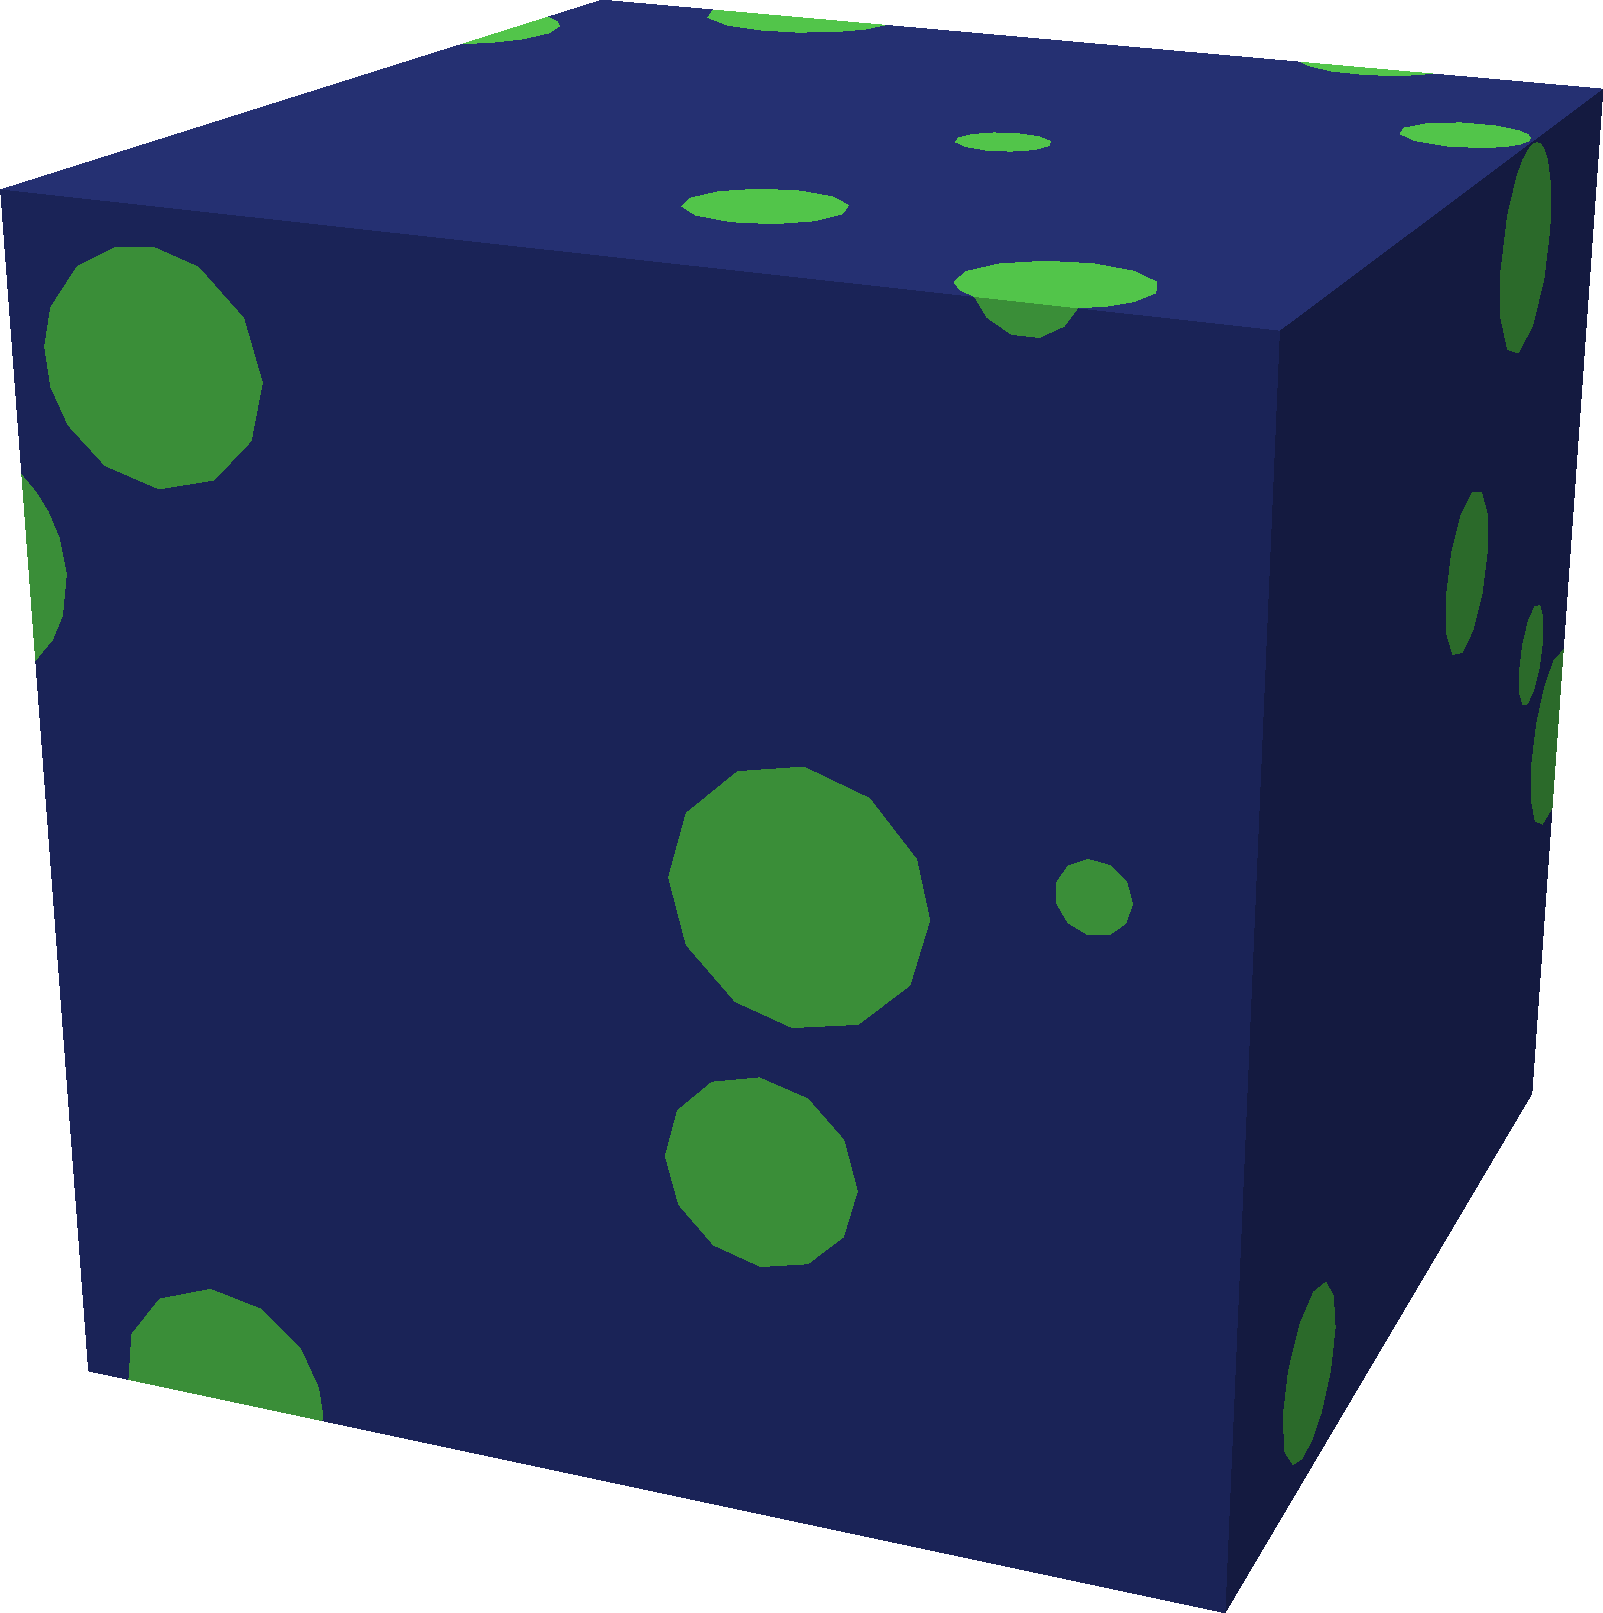
\includegraphics[width=0.45\linewidth]{rve6.png}
 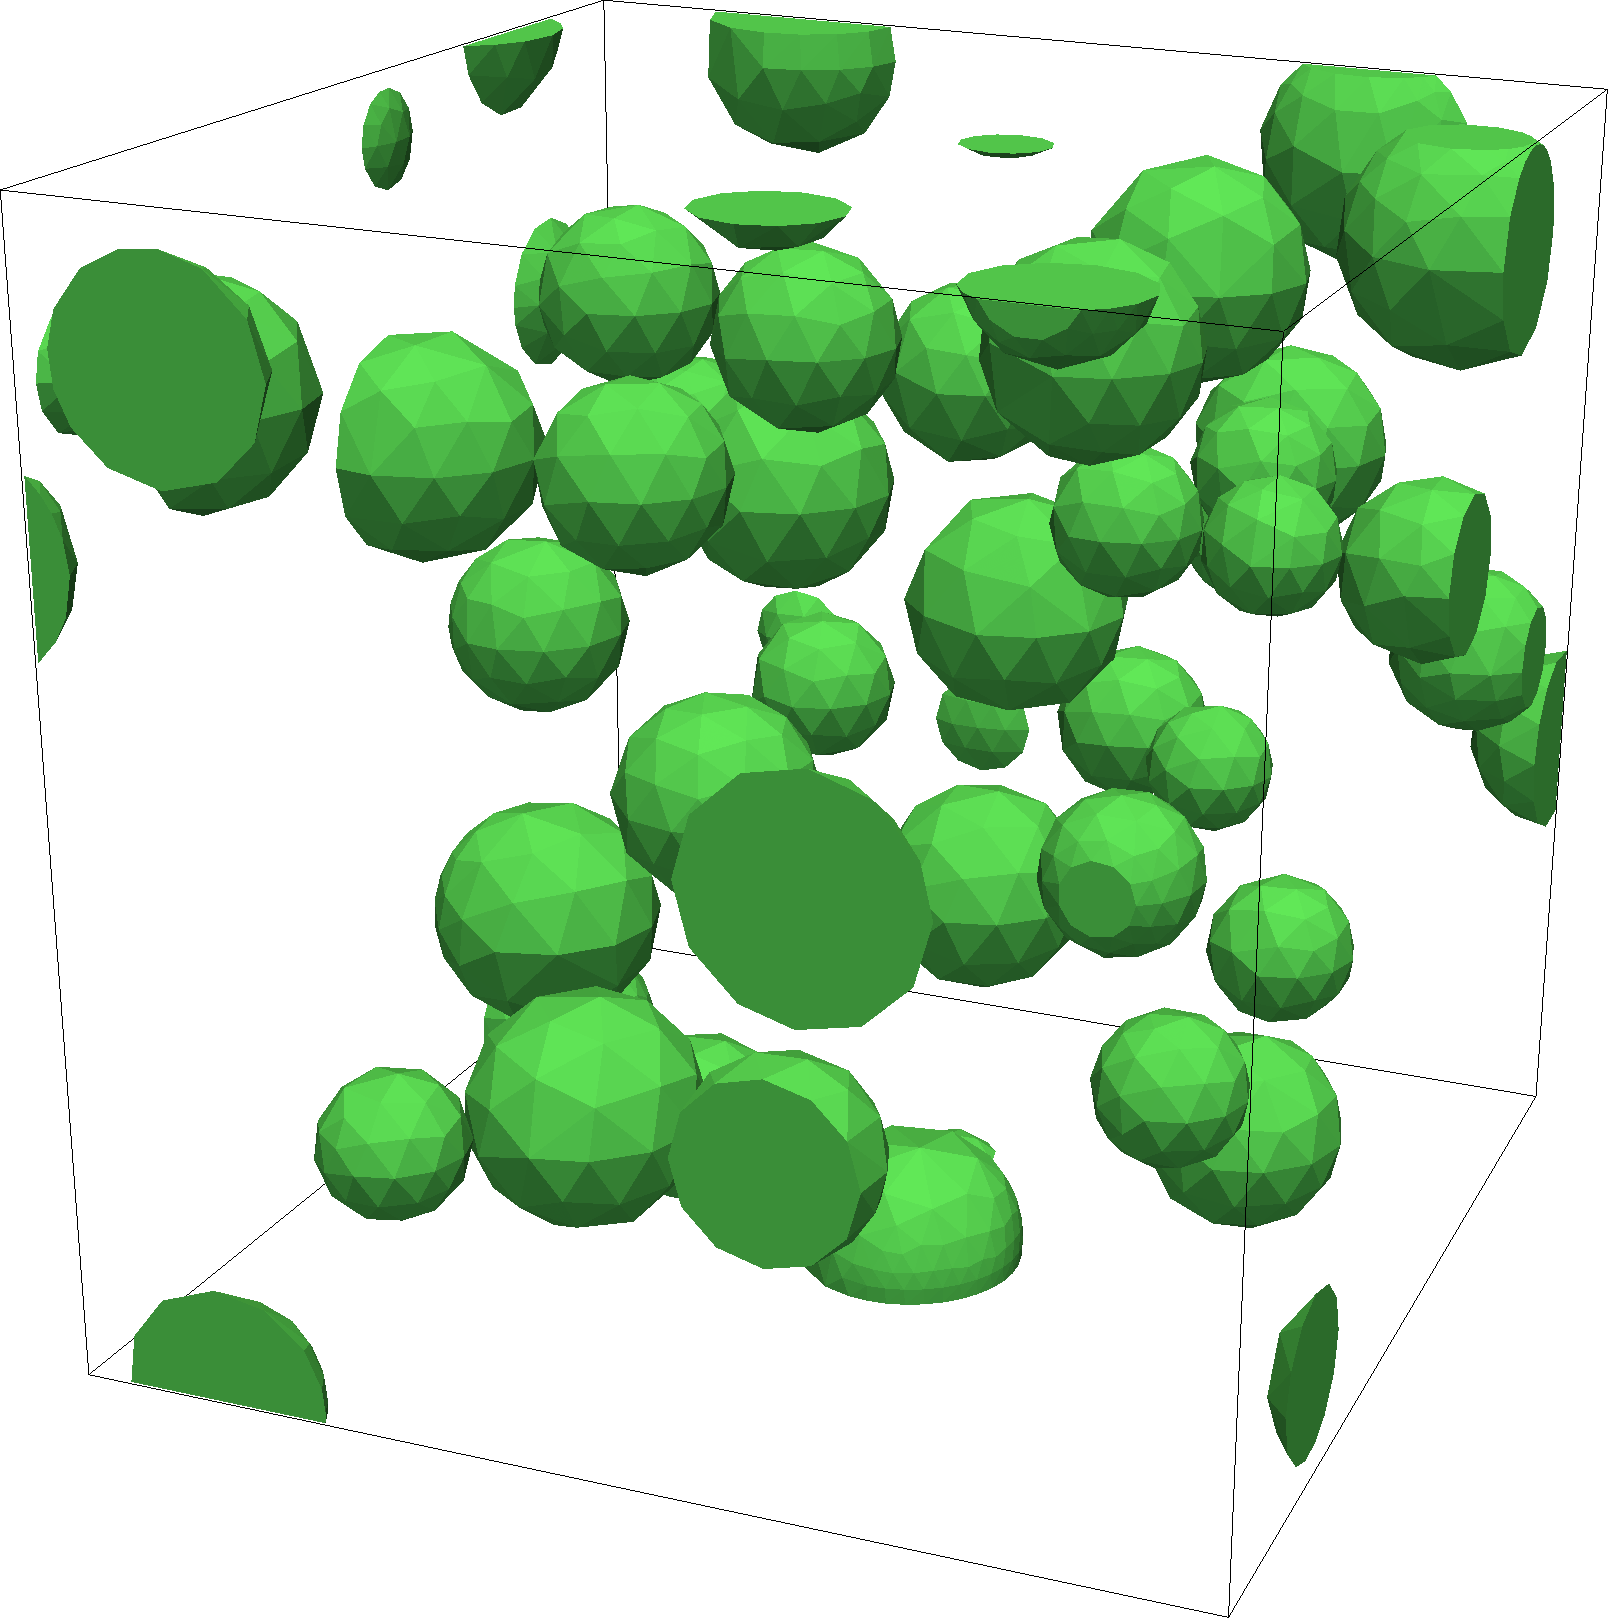
\includegraphics[width=0.45\linewidth]{rve6_inc.png}
\caption{A sample RVE of the dimensions $6\times6\times6$ shown with and without the matrix material visible.}
\label{fig:initial_rve6}
\end{figure}

\begin{figure}[htpb!]
\centering
 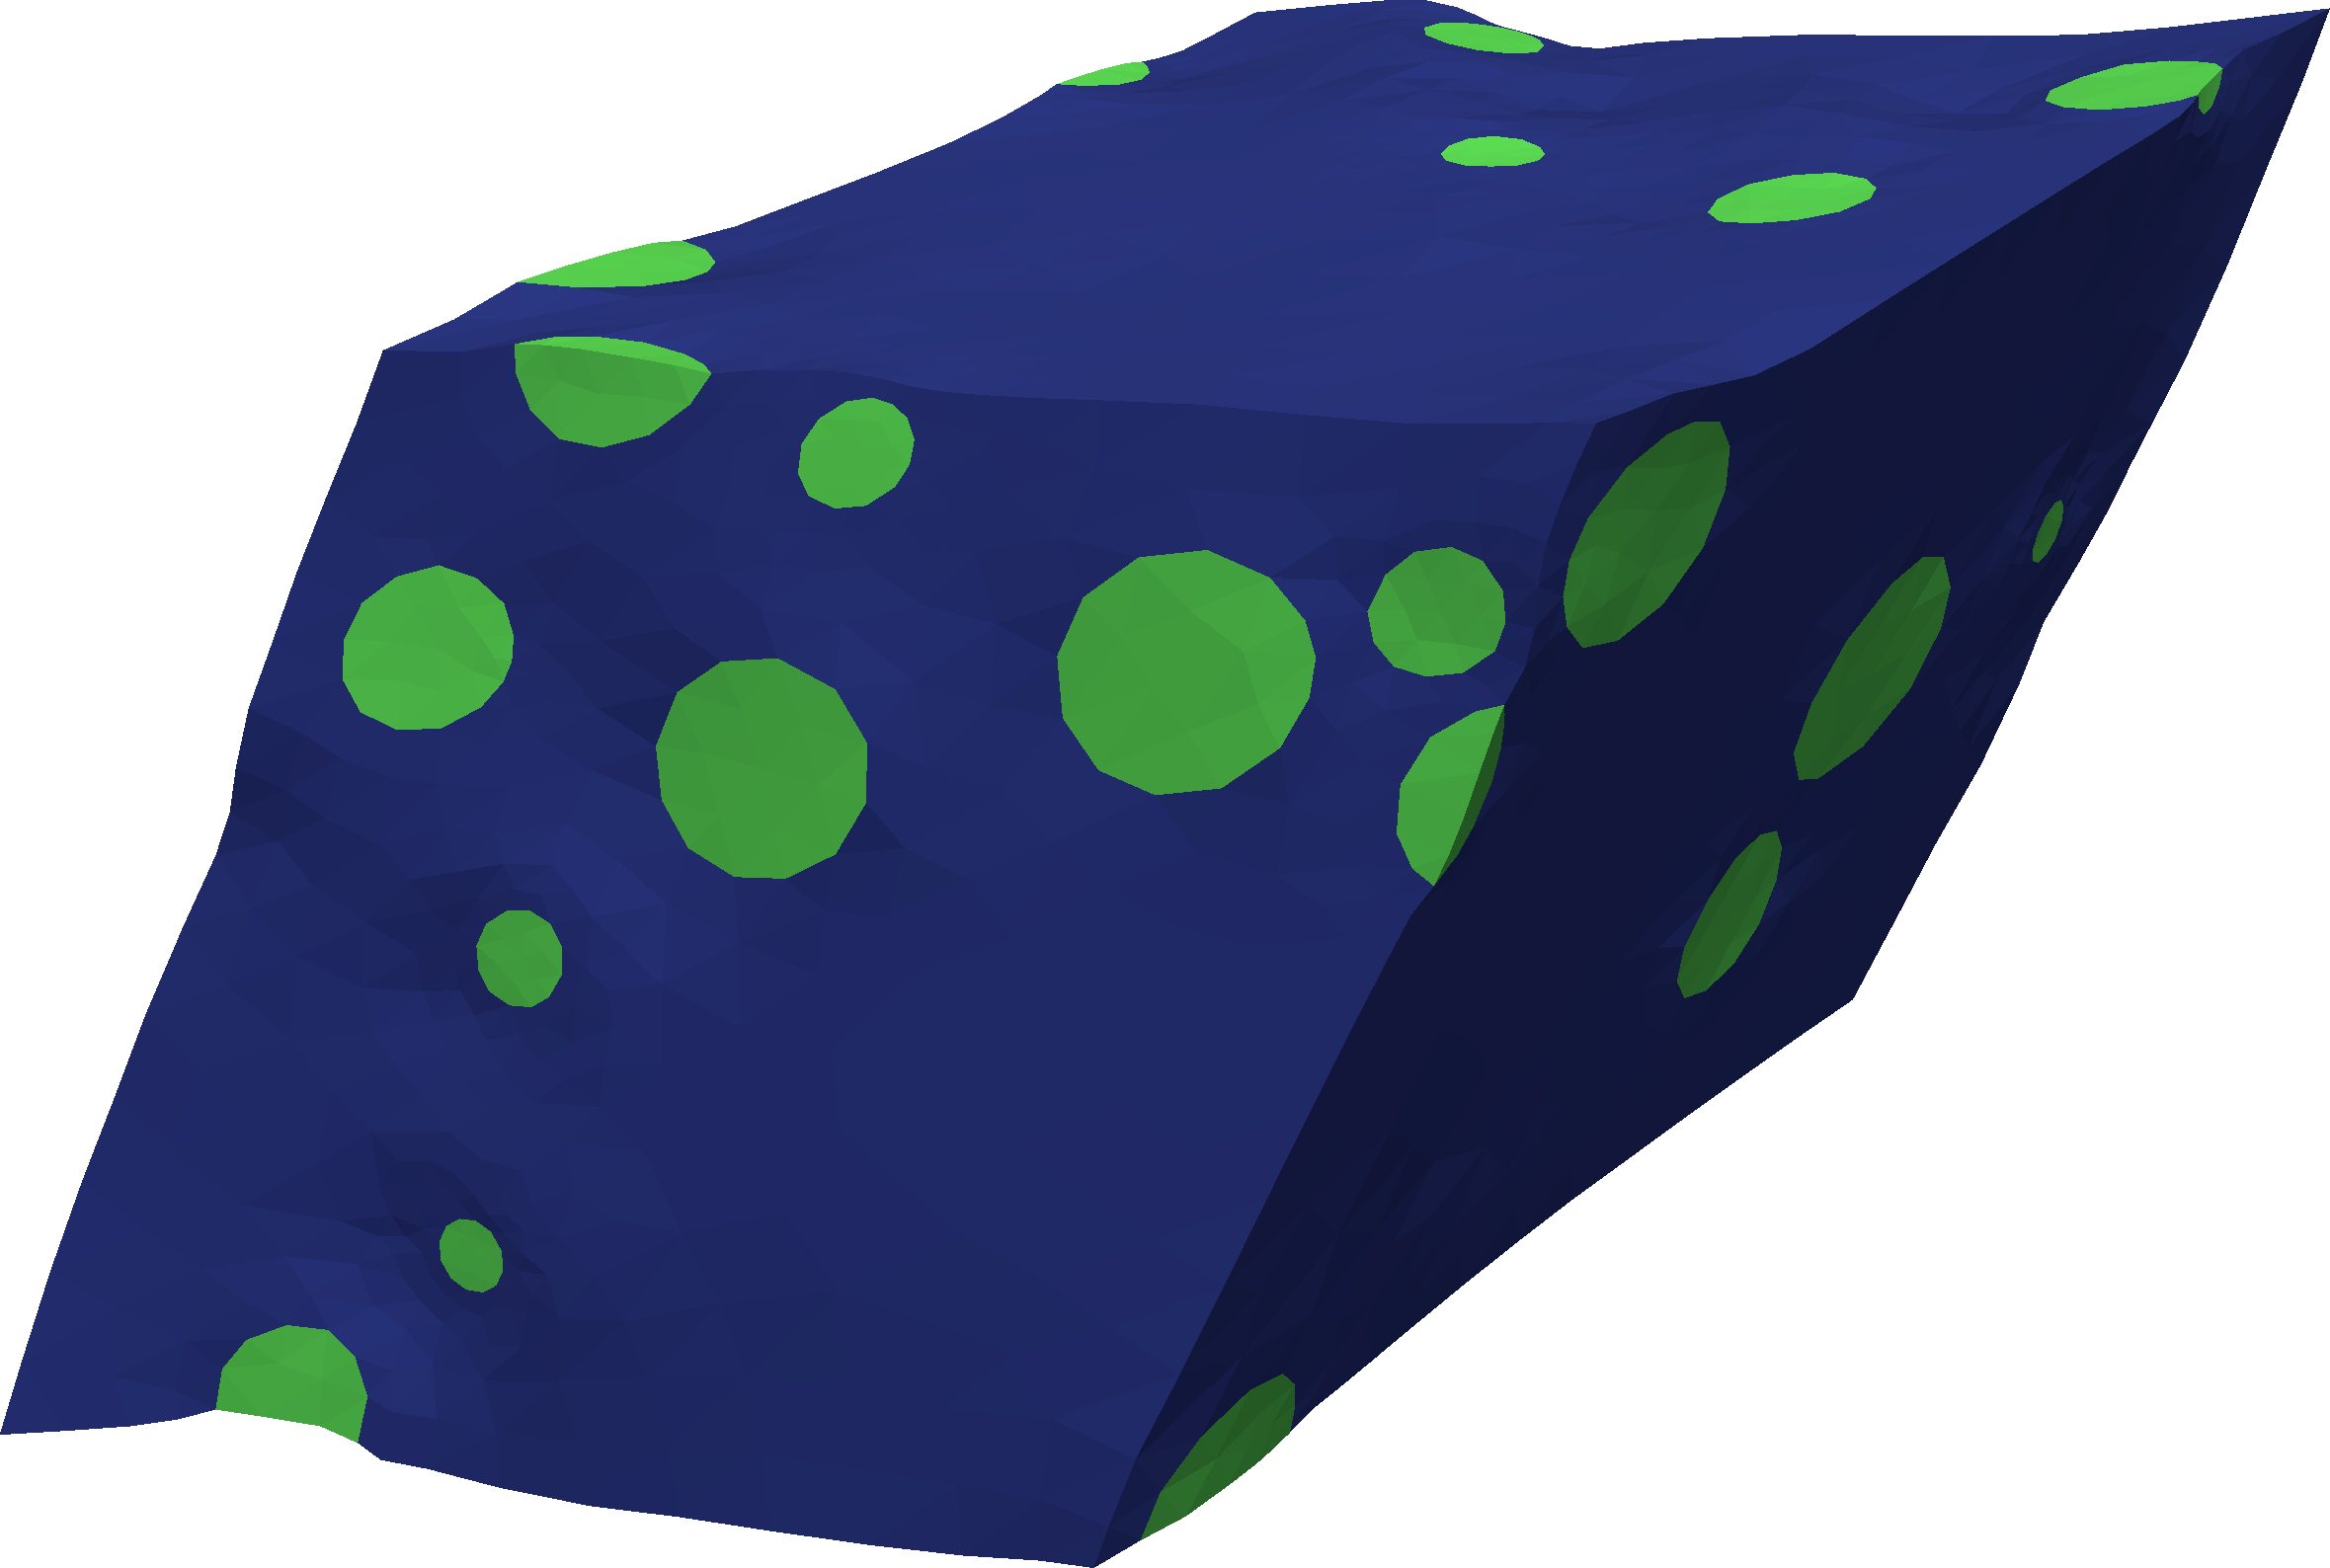
\includegraphics[width=0.7\linewidth]{rve6_def.png}
\caption{A sample SVE subject to Neumann boundary conditions and macroscopic shear $\bar{\epsilon}_{\dev,ij} = 0.4(1 - \delta_{ij})$.}
\label{fig:def_rve6}
\end{figure}

The SVE contains on average 10\% spherical inclusions with a mean diameter of one length unit.
A sample SVE is shown in \cref{fig:initial_rve6}.
The elements are linear tetrahedrons with bubble function for the displacement.
A convergence study was performed for the Dirichlet and Neumann boundary conditions where and the results are show in \cref{fig:SVE_comp}.
\begin{figure}[H]
\centering
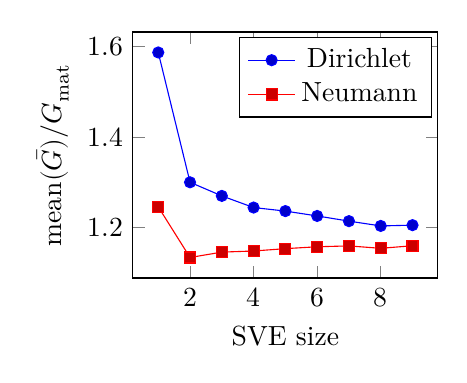
\begin{tikzpicture}
  \begin{axis}[ width=0.45\linewidth, xlabel=SVE size, ylabel=$\mathop{\mathrm{mean}}(\bar{G})/G_\mathrm{mat}$]
  \addplot table[color=blue,x=size,y=d_mean] {
size d_mean d_var
1.000000   1.586624   0.489829
2.000000   1.299371   0.029517
3.000000   1.269267   0.007279
4.000000   1.243507   0.002562
5.000000   1.235669   0.000874
6.000000   1.224925   0.000534
7.000000   1.213449   0.000258
8.000000   1.202848   0.000205
9.000000   1.204560   0.000033
  };
 \addlegendentry{Dirichlet}
  \addplot table[color=red,x=size,y=n_mean] {
size n_mean n_var
1.000000   1.245017   0.110729
2.000000   1.133016   0.006438
3.000000   1.144928   0.002252
4.000000   1.147371   0.001132
5.000000   1.152570   0.000572
6.000000   1.156771   0.000293
7.000000   1.158645   0.000139
8.000000   1.153319   0.000129
9.000000   1.158993   0.000039
  };
\addlegendentry{Neumann}
  \end{axis}
\end{tikzpicture}
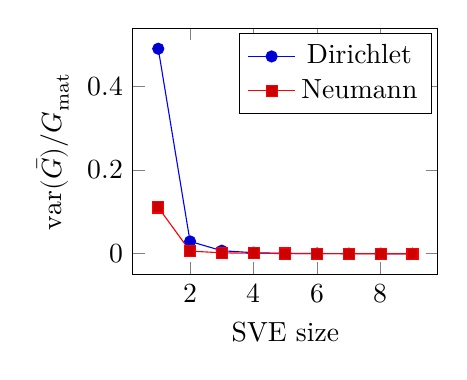
\begin{tikzpicture}
  \begin{axis}[ width=0.45\linewidth,  xlabel=SVE size, ylabel=$\mathop{\mathrm{var}}(\bar{G})/G_\mathrm{mat}$]
  \addplot table[color=blue,x=size,y=d_var] {
size d_mean d_var
1.000000   1.586624   0.489829
2.000000   1.299371   0.029517
3.000000   1.269267   0.007279
4.000000   1.243507   0.002562
5.000000   1.235669   0.000874
6.000000   1.224925   0.000534
7.000000   1.213449   0.000258
8.000000   1.202848   0.000205
9.000000   1.204560   0.000033
  };
\addlegendentry{Dirichlet}
  \addplot table[color=red,x=size,y=n_var] {
size n_mean n_var
1.000000   1.245017   0.110729
2.000000   1.133016   0.006438
3.000000   1.144928   0.002252
4.000000   1.147371   0.001132
5.000000   1.152570   0.000572
6.000000   1.156771   0.000293
7.000000   1.158645   0.000139
8.000000   1.153319   0.000129
9.000000   1.158993   0.000039
  };
\addlegendentry{Neumann}
  \end{axis}
\end{tikzpicture}
\caption{Statistical comparison between Neumann and Dirichlet boundary conditions}
\label{fig:SVE_comp}
\end{figure}




%[ 0.48982921  0.02951732  0.0072791   0.00256187  0.00087397  0.00053358]
%[ 0.1107292   0.00643845  0.00225217  0.00113156  0.00057236  0.00029335]


\section{Conclusions and outlook}
In this paper we have introduced a variationally consistent homogenization scheme for macroscopically incompressible micro structures.
We have shown the bounds for the periodic SVE by deriving the Dirichlet and Neumann boundary conditions.
The method is suitable whenever an SVE exhibit near or complete incompressibility, and works seamlessly if an SVE transitions from compressible to incompressible response.

The computational cost of the Neumann boundary condition is equivalent to that of the classical, compressible, Neumann boundary condition.
The Dirichlet boundary condition requires an additional, global, unknown to relax the volumetric deformation, which has a noticeable computational cost compared to the classical, compressible, Dirichlet boundary condition.
%\clearpage
%\printbibliography

\bibliography{Boundary_representation,Boundary_potentials,Multiscale,FEM_Software,Sintering,Mesh}
\bibliographystyle{plain}

%\bibliographystyle{elsarticle-num}
%\bibliography{ref_sintering}
%\bibliography{ref_multiscale}

%
%To be included?\\[1em]
% 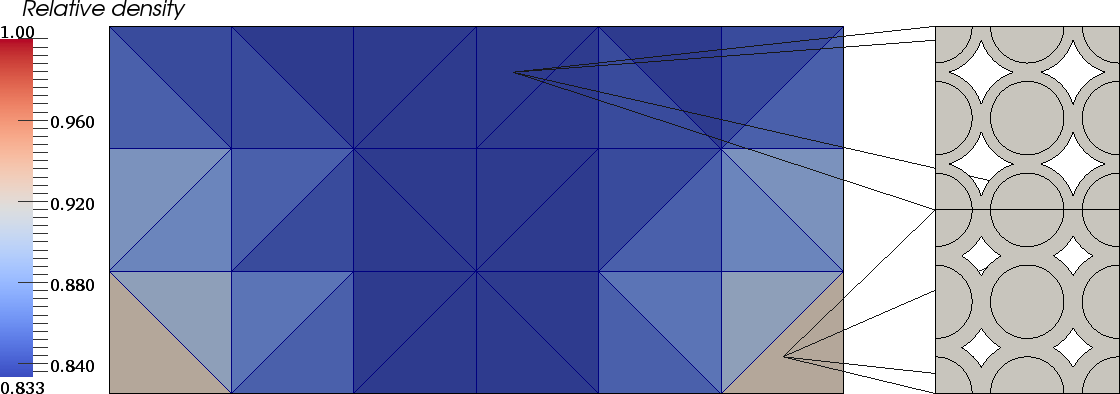
\includegraphics[width=0.9\linewidth]{figures/macro_sintering_2x2.0000}\\
% $\longrightarrow$\\[0.5em]
% 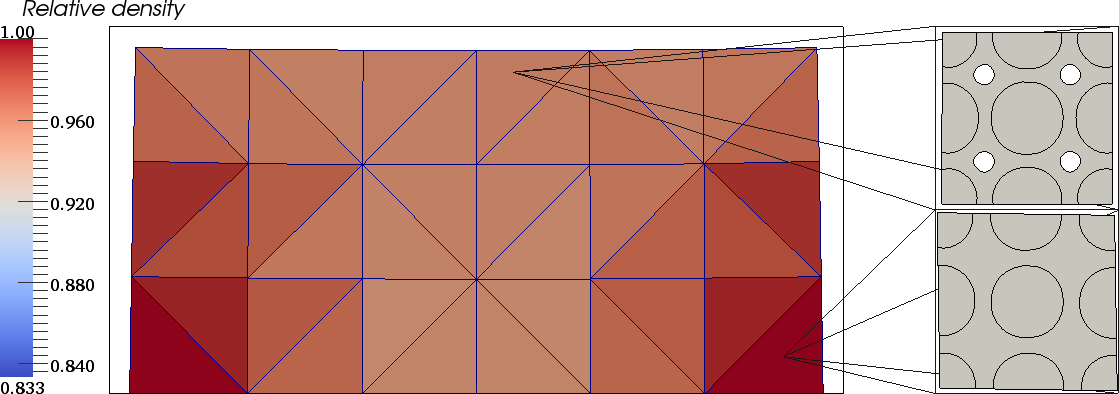
\includegraphics[width=0.9\linewidth]{figures/macro_sintering_2x2.0176}

\appendix
\setcounter{equation}{0}
\renewcommand{\theequation}{A-\arabic{equation}}

\section{Appendix}

\subsection{Variationally Consistent Homogenization (VCH)}

\textbf{Skriv om utg\aa{}ende fr\aa{}n paper Statistical Bounds ...}

\subsubsection{VMS-approach -- Scale separation and homogenization}

Classical model-based homogenization can be formulated in the spirit of the Variational MultiScale method (VMS), c.f.\ \cite{Hughesetal1998}, \cite{LarsonMalqvist2007}.
We introduce the abbreviated notation $z = (\ta u, p) \in \set{Z} = \set U \times \set P$, where $\set Z$ represents the space of fine-scale (non-homogenized) solutions to the system \eqref{eq2},
which may conveniently be abbreviated in abstract form as the residual equation\footnote{Henceforth in this Appendix, we consider the abstract formulation of a multifield problem based on a given set of balance (or constraint) equations.
No explicit reference to the specific character of the underlying problem is made.}
%-------------------------------------------------------------------------------------------------------------------------------
\begin{align}
 R(z; \delta z) \defeq R_\Omega(z; \delta z) + R_\Gamma(z;\delta z) = 0\quad \forall\;\delta z\in \set Z^0
\label{eq:A1}
\end{align}
%-------------------------------------------------------------------------------------------------------------------------------
where $\set Z^0 = \set U^0 \times \set P$ is the test space and where each $\ta u\in \set U^0$ vanishes on the Dirichlet part of $\Gamma$.

A multiscale formulation of \eqref{eq:A1} is defined by the hierarchical split $\set Z = \set Z^\macro \oplus \set Z^\fluct$, where $\set Z^\macro$ contains smooth macroscale functions and $\set Z^\fluct$ is the hierarchical complement of $\set Z^\macro$ that, typically, represents the fine-scale features.
It is assumed that each $z\in \set Z$ can be split uniquely as $z = z^\macro + z^\fluct$ such that $z^\macro \in \set Z^\macro$ and $z^\fluct \in \set Z^\fluct$.
Therefore, solve $z^\macro \in \set Z^\macro$, $z^\fluct \in \set Z^\fluct$ such that \eqref{eq:A1} can be represented by the set of equations
%------------------------------------------------------------------------------------------------------------------------------------------------
\begin{subequations}\label{eq:A2}
\begin{alignat}{3}
\label{eq:A2a} & R(z^\macro + z^\fluct; \delta z^\macro) &&= 0 \quad &&\forall\;\delta z^\macro \in \set Z^{\macro,0}\\
\label{eq:A2b} & R(z^\macro + z^\fluct; \delta z^\fluct) &&= 0       &&\forall\;\delta z^\fluct \in \set Z^{\fluct}
\end{alignat}
\end{subequations}
%-----------------------------------------------------------------------------------------------------------------------------
Without introducing further assumptions (approximations), the dimension of the original problem has not changed, i.e.\ \eqref{eq:A2} represent two global problems whose solution requires the same computational effort as does \eqref{eq:A1}.
In order to reduce the problem dimension based on homogenization (via the assumption of scale separation), we introduce the following key assumptions:

\begin{itemize}
\item The integrand in the volume integrals is replaced by a running volume average on SVE's of the type
%----------------------------------------------------------------------------------------------------------------
\begin{equation}
    \homgen{f}(\ta{x}') \defeq \frac{1}{|\Omega_\rve(\ta{x}')|} \int_{\Omega_\rve(\ta{x}')} f \dif V, \quad \ta{x}'\in\Omega
\label{eq:A105}
\end{equation}
%----------------------------------------------------------------------------------------------------------------------
such that, typically, the residual in \eqref{eq:A2a} can be rewritten in terms of the contributions defined on each SVE as
%--------------------------------------------------------------------------------------------------------------------------
\begin{align}
\label{eq:A106} R_\Omega(z;\delta z) = \int_\Omega R_\rve(z;\delta z)(\bar{\ta x})\dif\Omega
\end{align}
%------------------------------------------------------------------------------------------------------------------------------
where $R_\rve$ is the RVE-residual that is localized to the Representative Volume Element (RVE).
In practice (in FE-analysis), quadrature is used such that the evaluation of $R_\rve$ is carried out only in the Gauss points.

Furthermore, we assume smoothness of boundary terms, such that $R_\Gamma(z; \delta z^\macro) \approx R_\Gamma(z^\macro;\delta z^\macro)$, i.e.\ no boundary homogenization.

\item Introduce local approximations for the fluctuation field $z^\fluct$ in the spirit of VMS.
This means that $z^\fluct \approx \tilde{z}^\fluct\{z^\macro\}\in\set{Z}_\rve^{\fluct}$ is the \emph{approximate} solution\footnote{Curly brackets $\{\bullet\}$ indicate implicit function.} of the fine-scale 
equation \eqref{eq:A2b} for given $z^\macro$, i.e.\ \eqref{eq:A2b} is replaced by ``closed'' RVE-problems (in the macroscale quadrature points) associated with a particular choice of boundary conditions on $\Omega_\rve$.
%    Find $\tilde z^\fluct\in\set{Z}_\rve^{\fluct}$ that solve
%%---------------------------------------------------------------------------------------------------------------------------------------------
%\begin{align}
%\label{eq:A107} \tilde{R}_\rve(z^\macro+\tilde{z}^\fluct\{z^\macro\};\delta z^\fluct) = 0\quad \forall\;\delta z^\fluct \in \set{Z}_\rve^{\fluct}
%\end{align}
%%--------------------------------------------------------------------------------------------------------------------------------
\end{itemize}
Returning to \eqref{eq:A2a}, we now replace this problem by the approximate, homogenized, problem
%---------------------------------------------------------------------------------------------------------------------------------------------
\begin{align}
\label{eq:A3} R(z^\macro+\tilde{z}^\fluct\{z^\macro\};\delta z^\macro) = \int_\Omega R_\rve(z^\macro+\tilde{z}^\fluct\{z^\macro\};\delta z^\macro)(\bar{\ta x})\dif\Omega
 + R_\Gamma(z^\macro, \delta z^\macro) = 0 \quad \forall\;\delta z^\macro \in \set Z^{\macro,0}
\end{align}
%--------------------------------------------------------------------------------------------------------------------------------
which has the same dimension as \eqref{eq:A2a}.
We note that \eqref{eq:A3} represents a valid homogenization problem for any given choice of $\set{Z}_\rve^{\fluct}$; however, to preserve typical Galerkin properties, such as symmetry of the macroscale tangent operator when such symmetry is inherent in the underlying fine-scale problem, it is crucial to satisfy the VCMC.

\subsubsection{Variationally Consistent Macrohomogeneity Condition (VCMC)}

We shall assume that there exists a potential $\Pi(z)$ such that \eqref{eq:A3} represents the stationary point of $\Pi(z)$, i.e.\ it is assumed that
%---------------------------------------------------------------------------------------------------------------------------------------
\begin{align}
\label{eq:A4} R(z;\delta z) = \Pi'(z;\delta z) \defeq \frac{\dif}{\dif\epsilon}\Pi(z+\epsilon\delta z)|_{\epsilon = 0} = 0\quad \forall\;\delta z \in \set Z^0
\end{align}
%------------------------------------------------------------------------------------------------------
Next, we introduce the crucial \emph{approximation} (restriction) $z \approx z^\macro + \tilde{z}^\fluct\{z^\macro\}$ before evaluation of the stationarity conditions, whereby we obtain
%---------------------------------------------------------------------------------------------------------------------------------------
\begin{align}
\label{eq:A5} \Pi_{z^\macro}'\{z^\macro;\delta z^\macro\} & \defeq
\frac{\dif}{\dif\epsilon}\Pi(z^\macro+\epsilon \delta z^\macro+\tilde{z}^\fluct\{z^\macro+\epsilon \delta z^\macro\})|_{\epsilon = 0} \nonumber \\
& =
R(z^\macro + \tilde{z}^\fluct\{z^\macro\}; \delta z^\macro + (\tilde{z}^\fluct)'\{z^\macro;\delta z^\macro\}) = 0\quad \forall\;\delta z^\macro\in\set Z^{\macro,0}
\end{align}
%------------------------------------------------------------------------------------------------------------------------------------------
where $(\tilde{z}^\fluct)'\{z^\macro;\delta z^\macro\}$ denotes the sensitivity (or directional derivative) of $\tilde z^\fluct$ for a variation $\delta z^\macro$ of the macroscale solution $z^\macro$.
Hence, the choice of test function in \eqref{eq:A5} is restricted as compared to \eqref{eq:A4}, and this restriction represents a ``generalized Galerkin property'' in terms of the underlying macroscale functions in $\set Z^\macro$.
Moreover, and most importantly, \eqref{eq:A5} is completely equivalent to the homogenized problem \eqref{eq:A3} if it is possible, for any given $z^\macro\in\set Z^{\macro}$, to satisfy the constraint
%---------------------------------------------------------------------------------------------------------------------------------------------
\begin{align}
\label{eq:A6a} R(z^\macro + \tilde z^\fluct\{z^\macro\}; (\tilde{z}^\fluct)'\{z^\macro;\delta z^\macro\}) = 0\quad \forall\;\delta z^\macro\in\set Z^{\macro,0}(z^\macro)
\end{align}
%-------------------------------------------------------------------------------------------------------------------------------------------------
or, equivalently, \marginpar{solution space $\tilde{\set Z}$??}
%---------------------------------------------------------------------------------------------------------------------------------------------
\begin{align}
\label{eq:A6b} R(z^\macro + \tilde z^\fluct\{z^\macro\}; \delta\tilde{z}^\fluct) = 0\quad \forall\;\delta \tilde{z}^\fluct\in\tilde{\set Z}'^{\fluct}(z^\macro)
\end{align}
%-------------------------------------------------------------------------------------------------------------------------------------------------
where the test space $\tilde{\set Z}'^{\fluct}(z^\macro)$, which is the tangent space to the approximation space, is defined as
%----------------------------------------------------------------------------------------------------------------
\begin{align}
    \tilde{\set{Z}}'^{\fluct}(z^\macro)\defeq\{\set{Z}^\fluct\ni \dif z^\fluct = (\tilde{z}^\fluct)'\{z^\macro;\dif z^\macro\},\,
    \dif z^\macro\in \set{Z}^{\macro,0}\}
\label{eq:A6c}
\end{align}
%----------------------------------------------------------------------------------------------------------------------
Hence, $\dif \tilde{z}^\fluct\in\tilde{\set{Z}}'^{\fluct}(z^\macro)$ is the sensitivity of the fluctuation field $\tilde{z}^\fluct$ for differential changes of the macroscale field $z^\macro$ within the considered SVE.
It is computed from the tangent problem that is associated with the RVE-problem.
%as follows: \textbf{Galerkin property: $\tilde{\set{Z}}'^{\fluct}$ versus $\set{Z}_\rve^{\fluct}$ ?????}
%%---------------------------------------------------------------------------------------------------------------------------------------------
%\begin{align}
%\label{eq:A6d} (\tilde{R}_\rve)'(z;\delta z^\fluct,\dif z^\macro + \dif z^\fluct) = 0\quad \forall\;\delta z^\fluct\in\set{Z}_\rve^{\fluct}
%\end{align}
%%-------------------------------------------------------------------------------------------------------------------------------------------------
%where we introduced the tangent form
%%---------------------------------------------------------------------------------------------------------------------------------------------
%\begin{align}
%\label{eq:A6e} (\tilde{R}_\rve)'(z;\delta z,\dif z) \defeq \lim_{\epsilon \rightarrow 0}\frac{\dif}{\dif\epsilon}\tilde{R}_\rve(z+\epsilon\dif z;\delta z)
%\end{align}
%%-------------------------------------------------------------------------------------------------------------------------------------------------
%In other words, $\dif \tilde{z}^\fluct\{z^\macro;\dif z^\macro\}\in\tilde{\set{Z}}'^{\fluct}(\set{Z}^\macro)$ is solved from
%%---------------------------------------------------------------------------------------------------------------------------------------------
%\begin{align}
%\label{eq:A6f} (\tilde{R}_\rve)'(z;\delta z^\fluct,\dif \tilde{z}^\fluct) = -(\tilde{R}_\rve)'(z;\delta z^\fluct,\dif z^\macro) \quad
%\forall\;\delta z^\fluct\in\set{Z}_\rve^{\fluct}
%\end{align}
%%-------------------------------------------------------------------------------------------------------------------------------------------------
We refer to \eqref{eq:A6a} or \eqref{eq:A6b} as a ``variationally consistent (generalized) macro-homogeneity condition'' (VCMC).
Obviously, a sufficient condition for these identities to hold true is to require the RVE-residual to vanish on each RVE (in each quadrature point), i.e.\ to ensure that
%--------------------------------------------------------------------------------------------------------------------------------------
\begin{align}
\label{eq:A8} R_\rve(z^\macro + \tilde z^\fluct\{z^\macro\};(\tilde{z}^\fluct)'\{z^\macro;\delta z^\macro\}) = 0\quad \forall\;z^\macro,\delta z^\macro\in\set Z^{\macro}|_{\Omega_\rve}\times\set Z^{\macro,0}|_{\Omega_\rve}
\end{align}
%----------------------------------------------------------------------------------------------------------------------------------------------
An even stronger condition is to require that $R_\rve(z;\delta z^\fluct) = 0$ for \emph{any} $\delta z^\fluct$ in a given set of functions that is defined locally for the considered RVE without requiring any implicit (or explicit) 
coupling to the sensitivity field $(\tilde{z}^\fluct)'\{z^\macro;\delta z^\macro\}$, which obviously defines a restricted choice of test functions.
In such a case, the VCMC-condition can be identified as precisely the classical Hill-Mandel macrohomogeneity condition.

Finally, we remark that the VCMC ensures that the macroscale tangent operator becomes symmetrical, since it holds that
%---------------------------------------------------------------------------------------------------------------------------------------
\begin{align}
\label{eq:A9} R'(z;\delta z_1,\delta z_2) = \Pi''(z;\delta z_1,\delta z_2) \defeq \frac{\dif}{\dif\epsilon}\Pi'(z+\epsilon\delta z_2;\delta z_1)|_{\epsilon=0}\quad \forall\;\delta z_1,\delta z_2 \in \set Z^0
\end{align}
%------------------------------------------------------------------------------------------------------
With the introduced approximation $z^\fluct \approx \tilde{z}^\fluct\{z^\macro\}$, the test functions in \eqref{eq:A9} are chosen as
%---------------------------------------------------------------------------------------------------------------------------------------
\begin{align}
\label{eq:A10} \delta z_i \approx \delta z_i^\macro + (\tilde{z}^\fluct)'\{z^\macro;\delta z_i^\macro\} \quad \forall\;\delta z_i^\macro\in\set Z^{\macro,0}, \,\, i=1,2
\end{align}
%------------------------------------------------------------------------------------------------------------------------------------------


% \subsection{Weak format of RVE-problem REMOVE?!}
% \todo{no ref.}
% With the ansatz in (\ref{eq47a}), it follows that (\ref{eq51c}) can be rewritten
% %----------------------------------------------------------------------------
% \begin{equation}
%     d_\rve(\delta\ta{t},\ta{u}^\fluct) = 0
%     \quad \forall \delta\ta{t} \in \set{T}_\rve
% \label{eq:A11}
% \end{equation}
% %----------------------------------------------------------------------------
% Introduce the decomposition in (\ref{eq47c}) and choose $\delta\ta{t}=\delta\bar{\ts\tau}\cdot\ta{n}$ with $\delta\bar{\ts\tau}\in\set{R}^{3\times3}$.
% Inserting into (\ref{eq:A11}), we obtain
% %----------------------------------------------------------------------------
% \begin{equation}
%     d_\rve(\delta\bar{\ts\tau}\cdot\ta{n},\ta{u}^\fluct) = \delta\bar{\ts\tau}\dprod [
%     \underbrace{\frac{1}{\Omega_\rve}\int_{\Gamma_\rve^+} \jmp{\ta{u}^\fluct}\otimes\ta{n} \dif\Gamma}_{\ta{0} \mbox{ since } \delta\ta{u}^\fluct \in \set{U}_\rve^\fluct} ] = 0
% \label{eq:A12}
% \end{equation}

\subsection{Effective macroscale energy UPDATE}
\label{appendix:macroEnergy}
\textbf{not sure how to introduce this section}\todo{todo}
%----------------------------------------------------------------------------------------------------------------
\begin{equation}
    \bar{\ts\sigma}_\dev\{\bar{\ts\epsilon}_\dev,\bar{p}\} = \frac{\partial \bar{\psi}_\rve\{\bar{\ts\epsilon}_\dev,\bar{p}\}}{\partial \bar{\ts\epsilon}_\dev}, \quad
     \bar{e}\{\bar{\ts\epsilon}_\dev,\bar{p}\} = \frac{\partial \bar{\psi}_\rve\{\bar{\ts\epsilon}_\dev,\bar{p}\}}{\partial \bar{p}}
\end{equation}
%----------------------------------------------------------------------------------------------------------------------
where we can explicitly express each component of the macroscale deviatoric stress tensor such that $\bar{\sigma}_{\dev,i} \defeq \bar{\ts\sigma}_\dev \dprod \ts E_{i}$
\begin{multline}
  \bar{\sigma}_{\dev,i}\{\bar{\ts\epsilon}_\dev,\bar{p}\} = \underbrace{a_\rve(\ta u; (\ta u)'_{\epsilon_{\dev,i}}) + b_\rve(p, (\ta u)'_{\epsilon_{\dev,i}}) + d_\rve(\ta t, (\ta u)_{\epsilon_{\dev,i}}')}_{=0} + \underbrace{b_\rve((p)_p', \ta u) + c_\rve^*(p; (p)_{\epsilon_{\dev,i}}')}_{=0}
\\
+ \underbrace{\bar{p}\,(\bar{e})_{\epsilon_{\dev,i}}' - d_\rve(\ta t, (\bar{e})_{\epsilon_{\dev,i}}'\ta x_\mean)}_{=0} + \underbrace{d_\rve((\ta t)_{\epsilon_{\dev,i}}', \ta u - \bar{\ts\epsilon}_\dev\cdot[\ta x - \bar{\ta x}] - \bar{e}\,\ta x_\mean)}_{=0}
\\
 - d_\rve(\ta t, \ts E_{i}\cdot[\ta x - \bar{\ta x}]_\dev) = - d_\rve(\ta t, \ts E_{i}\cdot[\ta x - \bar{\ta x}]) = a_\rve(\ta u, \ts E_{i}\cdot[\ta x - \bar{\ta x}])
\end{multline}
and
\begin{multline}
  \bar{e}\{\bar{\ts\epsilon}_\dev,\bar{p}\} = \underbrace{a_\rve(\ta u; (\ta u)'_p) + b_\rve(p, (\ta u)'_p) + d_\rve(\ta t, (\ta u)_p')}_{=0} + \underbrace{b_\rve((p)_p', \ta u) + c_\rve^*(p; (p)_p')}_{=0}
\\
 + \underbrace{\bar{p}\,(\bar{e})_p' - d_\rve(\ta t, (\bar{e})_p'\ta x_\mean)}_{=0} + \underbrace{d_\rve((\ta t)_p', \ta u - \bar{\ts\epsilon}_\dev\cdot[\ta x - \bar{\ta x}] - \bar{e}\,\ta x_\mean)}_{=0} + \bar{e} = \bar{e}
\end{multline}
where we have used the equilibrium state in \cref{eq:rveStat} by choosing the test functions correspondingly; i.e.\ $\delta\ta u = (\ta u)_{pz}'$.

%----------------------------------------------------------------------------

%The purpose is to show that the consistency condition \cref{eq22} is satisfied a priori for the proposed functionals in \cref{eq23}.To this end, for $\ta{u}^\macro$ given in \cref{eq12}, we obtain
%%----------------------------------------------------------------------------
%\begin{eqnarray}
%    \bar{\ta{u}}_\rve(\ta{u}^\macro)
%    & = &
%    \bar{\ta{u}}_\rve(\bar{\ta{u}}+\bar{\ts\epsilon}\cdot[\ta{x}-\bar{\ta{x}}]) =
%    \bar{\ta{u}} \left(\frac{1}{|\Gamma_\rve^\fluct|}\int_{\Gamma_\rve^\fluct} \dif S\right) +
%    \bar{\ts\epsilon} \cdot \left(\underbrace{\frac{1}{|\Gamma_\rve^\fluct|}\int_{\Gamma_\rve^\fluct} \left[\ta{x}-\bar{\ta{x}}\right] \dif S}_{=0}\right)
%    \nonumber \\
%    & = & \bar{\ta{u}}
%\label{eqA1}
%\end{eqnarray}
%%----------------------------------------------------------------------------

\newpage
\subsection{Unique decomposition}
\label{appendix:unique_decomposition}
Using the identities
\begin{align}
 \set R^{3\times3} &= \{ \frac{1}{\volume} \int_{\Omega_\rve} \ta v \outerp \diff \dif V \,|\quad \ta v \in[H^1(\Omega_\rve)]^3 \}
\\
 \set R^3 &= \{ \frac{1}{\volume} \int_{\Gamma_\rve} \ta v \dif V \,|\quad \ta v \in L_2(\Omega_\rve) \}
\\
 \set R &= \{ \frac{1}{\volume} \int_{\Omega_\rve} q \dif V \,|\quad q \in L_2(\Omega_\rve) \}
\\
 \set R^{3\times3} &= \{ \frac{1}{\volume} \int_{\Omega_\rve} \ta s \outerp \jmp{\ta x - \bar{\ta x}} \dif S \,|\quad \ta s \in [L_2(\Gamma_\rve^+)]^3 \}
\end{align}
we can obtain
\begin{align}
 
\end{align}


% Orthogonality of the constant parts and the fluctuation spaces $\set{U}_\rve^\fluct$, $\set{T}_\rve^\fluct$, $\set{P}_\rve^\fluct$.
% ???????
% In \cref{eq28c} $\set{T}_\rve^\fluct$ has a restriction $\int_{\Gamma_\rve^+} \ta{s}\outerp\jmp{\ta{x}-\bar{\ta{x}}} \dif S = \ta{0}$ and we can directly see that $\ta s = \ts\tau \cdot \ta n$ leads to $\ts\tau\cdot \int_{\Gamma_\rve^+} \ta n \outerp\jmp{\ta{x}-\bar{\ta{x}}} \dif S = \ts\tau$.
% It remains to show that the same function spaces are spanned, i.e.
\begin{align}
\set{U}_\rve &= \set{U}_\rve^\fluct \cup \{ \ta u = \ts H \cdot [\ta x - \bar{\ta x}] \,|\quad \ts H \in \set{R}^{3\times 3}\}
\\
\set{P}_\rve &= \set{P}_\rve^\fluct \cup \{ p = q \,|\quad q\in \set{R}\}
\\
\set{T}_\rve &= \set{T}_\rve^\fluct \cup \{ \ta s = \ts \tau \cdot \ta n \,|\quad \ts\tau \in \set{R}^{3\times 3}\}
\end{align}


To be removed:
\begin{align}
    \set{U}_\rve^\fluct &= \{\ta{v}\in [H^1(\Omega_\rve)]^{3} \,| \quad \frac{1}{|\Gamma_\rve|}\int_{\Gamma_\rve} \ta{v} \dif S = 0, \quad
    \frac{1}{\volume}\int_{\Omega_\rve} \ta{v}\outerp\diff \dif V = \ta{0} \}
\\
    \set{P}_\rve^\fluct &= \{q\in L_2(\Omega_\rve) \,| \quad \frac{1}{\volume}\int_{\Omega_\rve} q \dif V = 0 \}
\\
    \set{T}_\rve^\fluct &= \{\ta{s}\in [L_2(\Gamma_\rve^+)]^{3} \,| \quad \frac{1}{\volume}\int_{\Gamma_\rve^+} \ta{s}\outerp\jmp{\ta{x}-\bar{\ta{x}}} \dif S
    = \ta{0} \}
\end{align}
\begin{align}
    \set{U}_\rve &= \{\ta{v}\in [H^1(\Omega_\rve)]^{3} \,| \quad \frac{1}{|\Gamma_\rve|}\int_{\Gamma_\rve} \ta{v} \dif S = 0 \}
\\
    \set{P}_\rve &= \{q\in L_2(\Omega_\rve) \}
\\
    \set{T}_\rve &= \{\ta{s}\in [L_2(\Gamma_\rve^+)]^{3} \}
\end{align}


\newpage
\subsection{Sensitivity problem}
\label{appendix:sensitivity}

The deviatoric tensors can be expressed in a orthonormal base such that
\begin{subequations}
\begin{gather}
 \bar{\ts\sigma}_\dev = \sum_{i=1}^{n_{\mathrm{b}}} \bar{\sigma}_{\dev,i} \ts E_i,\quad \bar{\ts\sigma}_\dev \dprod \ts E_i = \bar{\sigma}_{\dev,i}
\label{eq:sigma_base} \\
 \bar{\ts\epsilon}_\dev = \sum_{i=1}^{n_{\mathrm{b}}} \bar{\epsilon}_{\dev,i} \ts E_i,\quad \bar{\ts\epsilon}_\dev \dprod \ts E_i = \bar{\epsilon}_{\dev,i}
\label{eq:d_base}
\end{gather}
\end{subequations}
where examples of (generally unsymmetric) deviatoric base dyads are $\ts E_i$ can be chosen in a cartesian basis as
\begin{equation}
\begin{gathered}
 \ts E_1 = \frac{1}{\sqrt{6}}\left[\begin{smallmatrix} 2 & 0 & 0\\ 0 & -1 & 0\\ 0 & 0 & -1\end{smallmatrix}\right],\;
 \ts E_2 = \left[\begin{smallmatrix} 0 & 0 & 0\\ 0 & 1 & 0 \\ 0 & 0 & -1\end{smallmatrix}\right],\;
 \ts E_3 = \left[\begin{smallmatrix} 0 & 1 & 0\\ 0 & 0 & 0 \\ 0 & 0 & 0\end{smallmatrix}\right],\;
 \ldots,\;
 \ts E_8 = \left[\begin{smallmatrix} 0 & 0 & 0\\ 0 & 0 & 0 \\ 0 & 1 & 0\end{smallmatrix}\right].
\end{gathered}
\end{equation}
Using these, the macroscopic tangents can as
\begin{align}
 \bar{\ts C}_\ded \defeq \;&\pd{\bar{e}}{\bar{\ts\epsilon}_\dev} = \sum_{i=1}^{n_\mathrm{b}} \pd{\bar{e}}{\bar{\epsilon}_{\dev,i}} \ts E_i\\
 \bar{\ts E}_\dep \defeq \;&\pd{\bar{\ts\sigma}_\dev}{\bar{p}} = \sum_{i=1}^{n_\mathrm{b}} \pd{\bar{\sigma}_{\dev,i}}{\bar{p}} \ts E_i\\
 \bar{\tf E}_\ded \defeq \;&\pd{\bar{\ts\sigma}_\dev}{\bar{\ts\epsilon}_\dev} =  \sum_{i,j=1}^{n_\mathrm{b}} \pd{\bar{\sigma}_{\dev,i}}{\bar{\epsilon}_{\dev,j}} \ts E_i \outerp \ts E_j
\end{align}
where the derivatives are obtained by doing computing the homogenized sensitivities
\begin{align}
 \bar{    C}_\dep &= \bar{e}_{\dep}\\
 \bar{\ts C}_\ded &= \sum_{i=1}^{n_\mathrm{b}} \bar{e}_{\ded}^{(i)}\;\ts E_i\\
 \bar{\ts E}_\dep &= \sum_{i=1}^{n_\mathrm{b}} \bar{\sigma}_{\dev,i,\dep}\;\ts E_i\\
 \bar{\tf E}_\ded &= \sum_{i,j=1}^{n_\mathrm{b}} \bar{\sigma}_{\dev,i,\ded}^{(j)}\;\ts E_i \outerp \ts E_j
\end{align}
from the perturbed sensitivities fields from the linearized form at equilibrium.

\newpage
\subsubsection{Periodic boundary condition}
Sensitivities for the volumetric strain, $\bar{e}_\ded^{(k)}$ and $\bar{e}_\dep$ , are obtain directly from sensitivity analysis.

Upon using the identity $\bar{\ts\sigma}_\dev=\frac{1}{\volume} \int_{\Gamma_\Box^+} \ts t \outerp \jmp{\ta x - \bar{\ta x}}\dif S + \bar{p}\ts I$, we obtain the sensitivity
%---------------------------------------------------------------------------------------
\begin{align}
    \dif\bar{\ts\sigma}_{\dev}
    & =
    \frac{1}{\volume} \int_{\Gamma_\Box^+} \dif\ts t \outerp \jmp{\ta x - \bar{\ta x}}\dif S + \dif\bar{p}\ts I
\nonumber \\
    &= 
    \underbrace{\frac{1}{\volume} \int_{\Gamma_\Box^+} \ts t_\ded^{(j)} \outerp \jmp{\ta x - \bar{\ta x}}\dif S}_{\bar{\ts\sigma}_{\dev,\ded}^{(k)}}\,\dif\bar{\epsilon}_{\dev,j} + 
    \underbrace{\left[\frac{1}{\volume} \int_{\Gamma_\Box^+} \ts t_\dep \outerp \jmp{\ta x - \bar{\ta x}}\dif S + \ts I \right]}_{\bar{\ts\sigma}_{\dev,\dep}}\dif\bar{p}
\end{align}
where $\bar{\sigma}_{\dev,i,\ded}^{(k)} = \bar{\ts\sigma}_{\dev,\ded}^{(k)} \dprod \ts E_i$ and $\bar{\sigma}_{\dev,i,\dep} = \bar{\ts\sigma}_{\dev,\dep} \dprod \ts E_i$.
Using the perturbations $\bar{\ts\epsilon}_{\dev} + \dif\bar{\ts\epsilon}_{\dev}$ and $\bar{p} + \dif\bar{p}$ in the linearized form of \cref{eq51} at equilibrium we obtain
\begin{subequations}
\begin{alignat}{3}
    (a_\rve)'(\ta{u};\delta\ta{u},\Delta\ta u) + b_\rve(\Delta p,\delta\ta{u}) + d_\rve(\Delta\ta{t},\delta\ta{u}) &= 0
    &\quad& \forall \delta\ta{u} &&\in \set{U}_\rve
\\
    b_\rve(\delta p,\Delta\ta{u}) + (c^*_\rve)'(p;\delta p, \Delta p) &= 0
    &\quad& \forall \delta p &&\in \set{P}_\rve
\\
    d_\rve(\delta\ta{t},\Delta\ta{u}) - d_\rve(\delta\ta{t},\Delta\bar{e}\,\ta{x}_\mean) &= d_\rve(\delta\ta{t},\dif\bar{\ts\epsilon}_\dev \cdot[\ta{x}-\bar{\ta{x}}])
    &\quad& \forall \delta\ta{t} &&\in \set{T}_\rve
\\
    - d_\rve(\Delta\ta{t},\delta\bar{e}\,\ta{x}_\mean) &=
    - \dif\bar{p}\,\delta\bar{e}
    &\quad& \forall \delta\bar{e} &&\in \set{R}
\end{alignat}
\end{subequations}
which must hold for any given $\dif\bar{\ts\epsilon}_{\dev}$ and $\dif\bar{p}$.
We thus consider the cases
\begin{itemize}
 \item $\dif\bar{\epsilon}_{\dev,k} = 1$, $\dif\bar{\epsilon}_{\dev,j} = 0$ for $j\neq k$ while $\dif\bar{p} = 0$: For $k = 1, \ldots, n_\mathrm{b}$, solve the sensitivities $\ta{u}_\ded^{(k)}$, $p_\ded^{(k)}$, $\ta{t}_{\ded}^{(k)}$, $\bar{e}_\ded^{(k)}$ from the system 
\end{itemize}
\begin{subequations}\label{eq:p_sensitivities_d}
\begin{alignat}{3}
    (a_\rve)'(\ta{u};\delta\ta{u},\ta{u}_\ded^{(k)}) + b_\rve(p_\ded^{(k)},\delta\ta{u}) + d_\rve(\ta{t}_{\ded}^{(k)},\delta\ta{u}) &= 0
    &\quad& \forall \delta\ta{u} &&\in \set{U}_\rve
\\
    b_\rve(\delta p,\ta{u}_\ded^{(k)}) + (c^*_\rve)'(p;\delta p, p_\ded^{(k)}) &= 0
    &\quad& \forall \delta p &&\in \set{P}_\rve
\\
    d_\rve(\delta\ta{t},\ta{u}_\ded^{(k)}) - d_\rve(\delta\ta{t},\bar{e}_\ded^{(k)}\,\ta{x}_\mean) &= d_\rve(\delta\ta{t}, \ts E_k \cdot[\ta{x}-\bar{\ta{x}}])
    &\quad& \forall \delta\ta{t} &&\in \set{T}_\rve
\\
    - d_\rve(\ta{t}_{\ded}^{(k)},\delta\bar{e}\,\ta{x}_\mean) &= 0
    &\quad& \forall \delta\bar{e} &&\in \set{R}
\end{alignat}
\end{subequations}
\begin{itemize}
\item $\dif\bar{p} = 1$ while $\dif\bar{\epsilon}_{\dev,k} = 0$: Solve the sensitivities $\ta{u}_\dep$, $p_\dep$, $\ta{t}_\dep$, $\bar{e}_\dep$ from the system 
\end{itemize}
\begin{subequations}\label{eq:p_sensitivities_p}
\begin{alignat}{3}
    (a_\rve)'(\ta{u};\delta\ta{u},\ta{u}_\dep) + b_\rve(p_\dep,\delta\ta{u}) + d_\rve(\ta{t}_\dep,\delta\ta{u}) &= 0
    &\quad& \forall \delta\ta{u} &&\in \set{U}_\rve
\\
    b_\rve(\delta p,\ta{u}_\dep) + (c^*_\rve)'(p;\delta p, p_\dep) &= 0
    &\quad& \forall \delta p &&\in \set{P}_\rve
\\
    d_\rve(\delta\ta{t},\ta{u}_\dep) - d_\rve(\delta\ta{t},\bar{e}_\dep\,\ta{x}_\mean) &= 0
    &\quad& \forall \delta\ta{t} &&\in \set{T}_\rve
\\
    - d_\rve(\ta{t}_\dep,\delta\bar{e}\,\ta{x}_\mean) &=
    - \delta\bar{e}
    &\quad& \forall \delta\bar{e} &&\in \set{R}
\end{alignat}
\end{subequations}
% The volumetric strain, $\bar{e}_{\ded}^{(k)}$ and $\bar{e}_{\dep}$, is solved for directly, and the deviatoric stress is post-processed as
% \begin{align}
%  \bar{\ts\sigma}_{\dev,\ded}^{(k)} &=  \frac{1}{\volume} \int_{\Gamma_\rve} \ta{t}_{\ded}^{(k)} \outerp [\ta x - \bar{\ta x}]\dif S + \bar{p}\ts I\\
%  \bar{\ts\sigma}_{\dev,\dep} &= \frac{1}{\volume} \int_{\Gamma_\rve} \ta{t}_{\dep} \outerp [\ta x - \bar{\ta x}]\dif S + \bar{p}\ts I
% \end{align}


\newpage
\subsubsection{Neumann boundary condition}
Sensitivities for stress, $\bar{\sigma}_{\dev,i,\ded}^{(k)}$ and $\bar{\sigma}_{\dev,i,\dep}$, are obtained directly from the solution.
For the sensitivities of the volumetric strain, we have
%---------------------------------------------------------------------------------------
\begin{align}
    \dif\bar{e}
    & = \dif \homgen{\ta u\cdot \diff}
    = \sum_j \underbrace{\homgen{\ta u_\ded^{(j)}\cdot\diff}}_{\displaystyle\bar{e}_\ded^{(j)}}\,\dif\bar{\epsilon}_{\dev,j} + 
      \underbrace{\homgen{\ta u_\dep\cdot\diff}}_{\displaystyle\bar{e}_\dep}\,\dif\bar{p}.
\end{align}

Using the perturbations $\bar{\ts\epsilon}_{\dev} + \dif\bar{\ts\epsilon}_{\dev}$ and $\bar{p} + \dif\bar{p}$ in the linearized form of \cref{eq67} at equilibrium we obtain
\begin{subequations}
\begin{alignat}{3}
    (a_\rve)'(\ta{u};\delta\ta{u}, \Delta\ta u) + b_\rve(\Delta p,\delta\ta{u}) +  d'_\rve(\Delta\bar{\ts\sigma}_\dev,\delta\ta{u}) &= - \dif\bar{p}\,\homgen{\delta\ta{u}\cdot\diff }
    & \quad & \forall \delta\ta{u} &&\in \set{U}_\rve
\\
    b_\rve(\delta p,\Delta\ta{u}) + (c^*_\rve)'(p;\delta p, \Delta p) &= 0
    & \quad & \forall \delta p &&\in \set{P}_\rve
\\
    d'_\rve(\delta\bar{\ts\sigma}_\dev,\Delta\ta{u}) &= - \dif\bar{\ts\epsilon}_\dev\dprod\delta\bar{\ts\sigma}_\dev
    & \quad & \forall \delta\bar{\ts\sigma}_\dev &&\in\set{R}^{3\times3}_\dev
\end{alignat}
\end{subequations}
which must hold for any given $\dif\bar{\epsilon}_{\dev,i}$ and $\dif\bar{p}$.
We thus consider the cases
\begin{itemize}
 \item $\dif\bar{\epsilon}_{\dev,k} = 1$, $\dif\bar{\epsilon}_{\dev,j} = 0$ for $j\neq k$ while $\dif\bar{p} = 0$: For $k = 1, \ldots, n_\mathrm{b}$, solve the sensitivities $\ta u_\ded^{(k)}$, $p_\ded^{(k)}$, $\bar{\sigma}_{\dev,i,\ded}^{(k)}$ from the system 
\end{itemize}
\begin{subequations}\label{eq:n_sensitivities_d}
\begin{alignat}{3}
    (a_\rve)'(\ta{u};\delta\ta{u}, \ta u_\dev^{(k)}) + b_\rve(p_\dev^{(k)},\delta\ta{u}) +  d'_\rve(\bar{\sigma}_{\dev,i,\dev}^{(k)}\ts E_i,\delta\ta{u}) &= 0
    & \quad & \forall \delta\ta{u} &&\in \set{U}_\rve
\\
    b_\rve(\delta p,\ta u_\dev^{(k)}) + (c^*_\rve)'(p;\delta p, p_\dev^{(k)}) &= 0
    & \quad & \forall \delta p &&\in \set{P}_\rve
\\
    d'_\rve(\delta\bar{\sigma}_{\dev,i} \ts E_i,\ta u_\dev^{(k)}) &= - \delta_{ik}\;\delta\bar{\sigma}_{\dev,i}
    & \quad & \forall \delta\bar{\sigma}_{\dev,i} &&\in\set{R}
\end{alignat}
\end{subequations}
\begin{itemize}
\item $\dif\bar{p} = 1$ while $\dif\bar{\epsilon}_{\dev,k} = 0$: Solve the sensitivities $\ta u_\dep$, $p_\dep$, $\bar\sigma_{\dev,i,\dep}$ from the system 
\end{itemize}
\begin{subequations}\label{eq:n_sensitivities_p}
\begin{alignat}{3}
    (a_\rve)'(\ta{u};\delta\ta{u}, \ta u_\dep) + b_\rve(p_\dep,\delta\ta{u}) +  d'_\rve(\bar\sigma_{\dev,i,\dep}\ts E_i,\delta\ta{u}) &= -\homgen{\delta\ta{u}\cdot\diff }
    & \quad & \forall \delta\ta{u} &&\in \set{U}_\rve
\\
    b_\rve(\delta p,\ta u_\dep) + (c^*_\rve)'(p;\delta p, p_\dep) &= 0
    & \quad & \forall \delta p &&\in \set{P}_\rve
\\
    d'_\rve(\delta\bar{\sigma}_{\dev,i}\ts E_i,\ta u_\dep) &= 0
    & \quad & \forall \delta\bar{\sigma}_{\dev,i} &&\in\set{R}
\end{alignat}
\end{subequations}
% The deviatoric stresses, $\bar{\sigma}_{\dev,i,\ded}^{(k)}$ and $\bar{\sigma}_{\dev,i,\dep}$, are solved for directly, and the volumetric strain is post-processed as
% \begin{align}
%  \bar{e}_{\ded}^{(k)} &= \homgen{\ta u_\ded^{(k)}\cdot\diff}\\
%  \bar{e}_\dep &= \homgen{\ta u_\dep \cdot\diff}
% \end{align}

\newpage
\subsubsection{Dirichlet boundary condition}
Sensitivities for the volumetric strain, $\bar{e}_\ded^{(k)}$ and $\bar{e}_\dep$ , are obtain directly from sensitivity analysis.
Upon using the identity $\bar{\ts\sigma}=\frac{1}{\volume} \int_{\Gamma_\Box} \ts t \outerp [\ta x - \bar{\ta x}]\dif S$, we deduce the component sensitivity
%---------------------------------------------------------------------------------------
\begin{align}
    \dif\bar{\sigma}_{\dev,i}
    & =
    \dif\bar{\ts\sigma}\dprod \ts E_i
    =
    \dif\left[\frac{1}{\volume} \int_{\Gamma_\Box} \ts t \cdot \ts E_i \cdot [\ta x - \bar{\ta x}]\dif S\right]
    = (a_\Box)'(\ta{u}; \ta{u}^{\macro(i)}_\dev,\dif\ta{u})
\nonumber \\
    & =
    \sum_j \underbrace{(a_\Box)'(\ta{u};\ta{u}^{\macro(i)}_\dev,\ta{u}^{\macro(j)}_\dev +
    \ta{u}^{\fluct(j)}_\ded)}_{\displaystyle \bar{\sigma}_{\dev,i,\ded}^{(j)}}
    \dif\bar{\epsilon}_{\dev,j}
% Second term
    + \underbrace{(a_\Box)'(\ta{u};\ta{u}^{\macro(i)}_\dev, \ta{u}^{\fluct}_\dep)}_{\displaystyle \bar{\sigma}_{\dev,i,\dep}}
    \dif\bar{p}
\end{align}
%---------------------------------------------------------------------------------------
where $\ta u^{\macro(i)}_\dev = \ts E_i \cdot[\ta x - \bar{\ta x}]$.

Using the perturbations $\bar{\ts\epsilon}_{\dev} + \dif\bar{\ts\epsilon}_{\dev}$ and $\bar{p} + \dif\bar{p}$ in the linearized form of \cref{eq:weak_form_dirichlet} at equilibrium we obtain
\begin{subequations}
\begin{alignat}{3}
    (a_\rve)'(\ta u;\delta\ta{u}^\fluct, \dif \bar{\ts\epsilon}_\dev\cdot[\ta x - \bar{\ta x}] + \Delta\ta{u}^\fluct) + b_\rve(\Delta p, \delta\ta{u}^\fluct) &= 0
    &\quad& \forall \delta\ta{u}^\fluct &&\in \set{U}_\rve^{\Dirichlet,0}
\\
    b_\rve(\delta p,\Delta\ta{u}^\fluct + \Delta\bar{e}\,\ta{x}_\mean) + (c^*_\rve)'(p;\delta p,\Delta p) &= 0
    &\quad& \forall \delta p &&\in \set{P}_\rve
\\
    b_\rve(\Delta p,\delta\bar{e}\,\ta{x}_\mean) &=
    - \dif\bar{p}\,\delta\bar{e}
    &\quad& \forall \delta\bar{e} &&\in \set{R}
\end{alignat}
\end{subequations}
which must hold for any given $\dif\bar{\epsilon}_{\dev,i}$ and $\dif\bar{p}$.
We thus consider the cases
\begin{itemize}
 \item $\dif\bar{\epsilon}_{\dev,k} = 1$, $\dif\bar{\epsilon}_{\dev,j} = 0$ for $j\neq k$ while $\dif\bar{p} = 0$: For $k = 1, \ldots, n_\mathrm{b}$, solve the sensitivities $\ta u_\ded^{\fluct(k)}$, $p_\ded^{(k)}$, $\bar{e}_{\ded}^{(k)}$ from the system 
\end{itemize}
\begin{subequations}\label{eq:d_sensitivities_d}
\begin{alignat}{3}
    (a_\rve)'(\ta{u};\delta\ta{u}^\fluct, \ta u_\ded^{\fluct(k)}) + b_\rve(p_\ded^{(k)},\delta\ta{u}^\fluct) &= -(a_\rve)'(\ta{u};\delta\ta{u}^\fluct, \ta{u}^{\macro(k)}_\dev)
    &\quad& \forall \delta\ta{u}^\fluct &&\in \set{U}_\rve^{\Dirichlet,0}
\\
    b_\rve(\delta p,\ta u_\ded^{\fluct(k)} + \bar{e}_{\ded}^{(k)}\,\ta{x}_\mean) + (c^*_\rve)'(p;\delta p,p_\ded^{(k)}) &= 0
    &\quad& \forall \delta p &&\in \set{P}_\rve
\\
    b_\rve(\Delta p,\delta\bar{e}\,\ta{x}_\mean) &= 0
    &\quad& \forall \delta\bar{e} &&\in \set{R}
\end{alignat}
\end{subequations}
\begin{itemize}
\item $\dif\bar{p} = 1$ while $\dif\bar{\epsilon}_{\dev,k} = 0$: Solve the sensitivities $\ta u_\dep^\fluct$, $p_\dep$, $\bar{e}_{\dep}$ from the system 
\end{itemize}
\begin{subequations}\label{eq:d_sensitivities_p}
\begin{alignat}{3}
    (a_\rve)'(\ta{u}^\macro + \ta{u}^\fluct;\delta\ta{u}^\fluct, \ta u_\dep^\fluct) + b_\rve(p_\dep,\delta\ta{u}^\fluct) &= 0
    &\quad& \forall \delta\ta{u}^\fluct &&\in \set{U}_\rve^{\Dirichlet,0}
\\
    b_\rve(\delta p,\ta u_\dep^\fluct) + b_\rve(\delta p,\bar{e}_{\dep}\,\ta{x}_\mean) + (c^*_\rve)'(p;\delta p,p_\dep) &= 0
    &\quad& \forall \delta p &&\in \set{P}_\rve
\\
    b_\rve(p_\dep,\delta\bar{e}\,\ta{x}_\mean) &= - \delta\bar{e}
    &\quad& \forall \delta\bar{e} &&\in \set{R}
\end{alignat}
\end{subequations}
% The volumetric strain, $\bar{e}_{\ded}^{(k)}$ and $\bar{e}_{\dep}$, is solved for directly, and the deviatoric stress is post-processed as
% \begin{align}
%  \bar{\ts\sigma}_{\dev,\ded}^{(k)} &=  \frac{1}{\volume} \int_{\Gamma_\rve} \ta{t}_{\ded}^{(k)} \outerp [\ta x-\bar{\ta x}]\dif S\\
%  \bar{\ts\sigma}_{\dev,\dep} &= \frac{1}{\volume} \int_{\Gamma_\rve} \ta{t}_{\dep} \outerp [\ta x-\bar{\ta x}]\dif S
% \end{align}

\end{document}